%% LyX 2.0.4 created this file.  For more info, see http://www.lyx.org/.
%% Do not edit unless you really know what you are doing.
\documentclass[11pt,english]{article}
\usepackage{mathpazo}
\usepackage[]{fontenc}
\usepackage[utf8]{inputenc}
\setlength{\parskip}{\smallskipamount}
\setlength{\parindent}{0pt}
\usepackage{babel}
\usepackage{verbatim}
\usepackage{url}
\usepackage{amssymb}
\usepackage{makeidx}
\makeindex
\usepackage{graphicx}
\usepackage{esint}
\usepackage[unicode=true,pdfusetitle,
 bookmarks=true,bookmarksnumbered=false,bookmarksopen=false,
 breaklinks=false,pdfborder={0 0 1},backref=false,colorlinks=false]
 {hyperref}
\usepackage{breakurl}

\makeatletter
%%%%%%%%%%%%%%%%%%%%%%%%%%%%%% Textclass specific LaTeX commands.
\usepackage{noweb}
\newenvironment{lyxcode}
{\par\begin{list}{}{
\setlength{\rightmargin}{\leftmargin}
\setlength{\listparindent}{0pt}% needed for AMS classes
\raggedright
\setlength{\itemsep}{0pt}
\setlength{\parsep}{0pt}
\normalfont\ttfamily}%
 \item[]}
{\end{list}}

\makeatother

\begin{document}

\title{Finite element code: PDE}


\author{David E. Stewart}


\date{July 9th, 2012}

\maketitle
\tableofcontents{}


\section{\label{sec:Overview}Overview}

\global\long\def\R{\mathbb{R}}
This describes a pure Matlab finite element code for two dimensional
problems. It is assumed that a triangulation of the domain is given
in the same format as the output from the Persson \& Strang Matlab
triangulation code \cite{ps:smgm}. That is, the basic triangulation
data is given in the form of a pair $(p,t)$ where $p$ is an array
of points: point $p_{i}$ is \texttt{p(i,:)}, while triangle $i$
is the triangle with vertices \texttt{p(j,:)}, \texttt{p(k,:)}, \texttt{p(l,:)}
where \texttt{j = t(i,1)}, \texttt{k = t(i,2)} and \texttt{l = t(i,3)}.
This can be generalized to tetrahedra in three dimensions, etc. This
also works well with the Matlab \texttt{\index{trimesh()}trimesh()}
function for plotting two-dimensional meshes.

There are a number of different element types, most notably \index{element!Lagrange}Lagrange
elements which represent scalar piecewise polynomials (that is, the
restriction of the basis functions to each triangle is a polynomial).
The simplest of these is the Lagrange piecewise linear element, but
quadratic and cubic Lagrangian elements have also been implemented.
Extensions to $C^{1}$ elements (such as Bell's triangle and the Argyris
element) are also planned, but not yet implemented. Code for the elements
can be found in Section~\ref{sec:Element-types}.

Since the values at certain points are shared by elements on different
(but touching) triangles, we need a way to determine when these values
are shared. This is done via a geometric feature hash table. Code
for these aspects can be found in Section~\ref{sec:Handling-geometric-features}.

The core routines are the assembly routines which form the matrices
and vectors for the linear systems to be solved. These are for both
the Galerkin and Petrov--Galerkin methods. Similar routines are provided
for handling boundary values and conditions. Code for matrix assembly
can be found in Section~\ref{sec:Matrix-assembly-code}. Part of
this process is the task of numerical integration. Integration rules
can be found in Section~\ref{sec:Numerical-integration}.

Testing codes can be found in Section~\ref{sec:Test-code}.


\subsection{\label{sub:Basic-organization}Basic organization}

Each element type must be able to compute the values of the basis
functions at each point of the reference triangle $\widehat{K}=\mbox{co}\left\{ \,(0,0),\,(1,0),\,(0,1)\,\right\} $,
along with the values of a number of \emph{operators} applied to the
basis functions. That is, for a point $\widehat{\mathbf{x}}\in\widehat{K}$
and basis function $\widehat{\phi}_{i}$ on $\widehat{K}$ we need
to be able to compute not only $\widehat{\phi}_{i}(\widehat{\mathbf{x}})$,
but also $\mathcal{A}\widehat{\phi}_{i}(\widehat{\mathbf{x}})$ where
$\mathcal{A}=\partial/\partial x_{1}$, $\mathcal{A}=\partial/\partial x_{2}$;
sometimes higher order derivatives are also necessary, such as for
4th order PDEs. In that case, each element can also compute $\mathcal{A}\widehat{\phi}_{i}(\widehat{\mathbf{x}})$
where $\mathcal{A}=\partial^{2}/\partial x_{1}^{2}$, $\mathcal{A}=\partial^{2}/\partial x_{1}\,\partial x_{2}$
and $\mathcal{A}=\partial^{2}/\partial x_{2}^{2}$. The ordering of
these operators is essentially fixed across the different element
types.

There are also elements for providing vector-valued basis functions,
in which case we also need to use different operators: $\mathcal{A}\widehat{\phi}_{i}(\widehat{\mathbf{x}})=\widehat{\phi}_{i}(\widehat{\mathbf{x}})\cdot\mathbf{e}_{1}$,
$\mathcal{A}\widehat{\phi}_{i}(\widehat{\mathbf{x}})=\widehat{\phi}_{i}(\widehat{\mathbf{x}})\cdot\mathbf{e}_{2}$,
$\mathcal{A}\widehat{\phi}_{i}(\widehat{\mathbf{x}})=\partial\widehat{\phi}_{i}(\widehat{\mathbf{x}})/\partial x_{1}\cdot\mathbf{e}_{1}$,
etc. 

Basis functions on the reference element $\widehat{K}$ are used to
create basis functions on the actual elements $K=\mbox{co}\left\{ \,\mathbf{p}_{j},\,\mathbf{p}_{k},\,\mathbf{p}_{\ell}\,\right\} $
by means of an affine transformation $\widehat{\mathbf{x}}\mapsto\mathbf{x}=T_{K}\widehat{\mathbf{x}}+\mathbf{b}_{K}$
with $T_{K}$ and $\mathbf{b}_{K}$ computed from $\mathbf{p}_{j},\,\mathbf{p}_{k},\,\mathbf{p}_{\ell}$.
This also transforms that values of $\mathcal{A}'\widehat{\phi}_{i}(\widehat{\mathbf{x}})$
to compute $\mathcal{A}\phi_{i}(\mathbf{x})$: $\phi_{i}(\mathbf{x})=\widehat{\phi}_{i}(\widehat{\mathbf{x}})$,
but 
\[
\frac{\partial\phi_{i}}{\partial x_{1}}(\mathbf{x})=\frac{\partial\widehat{\phi}_{i}}{\partial\widehat{x}_{1}}(\widehat{\mathbf{x}})\frac{\partial\widehat{x}_{1}}{\partial x_{1}}(\mathbf{x})+\frac{\partial\widehat{\phi}_{i}}{\partial\widehat{x}_{2}}(\widehat{\mathbf{x}})\frac{\partial\widehat{x}_{2}}{\partial x_{1}}(\mathbf{x}),
\]
for example. The derivatives $\partial\widehat{x}_{i}/\partial x_{i}$
are entries of the $T_{K}$ matrix. In fact, 
\[
\nabla\phi_{i}(\mathbf{x})=(T_{K})^{T}\nabla\widehat{\phi}_{i}(\widehat{\mathbf{x}}).
\]


The matrix entries are formed by means of integrals
\begin{eqnarray*}
a_{ij} & = & \int_{\Omega}\sum_{\mathcal{A},\mathcal{B}}c_{\mathcal{A},\mathcal{B}}(\mathbf{x})\,\mathcal{A}\phi_{i}(\mathbf{x})\,\mathcal{B}\phi_{j}(\mathbf{x})\, d\mathbf{x}\\
 & = & \sum_{K}\int_{K}\sum_{\mathcal{A},\mathcal{B}}c_{\mathcal{A},\mathcal{B}}(\mathbf{x})\,\mathcal{A}\phi_{i}(\mathbf{x})\,\mathcal{B}\phi_{j}(\mathbf{x})\, d\mathbf{x}.
\end{eqnarray*}
The sum over $\mathcal{A}$ and $\mathcal{B}$ is over all the operators
used to define the Galerkin form of the partial differential equations;
the sum over $K$ is the sum over all the triangles of the triangulation.
To compute the integral over $K$ we use rules for integration over
the reference triangle $\widehat{K}$. 

For the Petrov--Galerkin method, we can use different basis functions
(and thus different element types), but they must be based on the
same triangulation:
\[
b_{ij}=\sum_{K}\int_{K}\sum_{\mathcal{A},\mathcal{B}}c_{\mathcal{A},\mathcal{B}}(\mathbf{x})\,\mathcal{A}\psi_{i}(\mathbf{x})\,\mathcal{B}\phi_{j}(\mathbf{x})\, d\mathbf{x}.
\]
There are also matrix assembly routines for boundaries. Boundaries
of two-dimensional regions are given as sets of edges (each edge being
a pair of indexes into the point array \texttt{p}).


\subsection{\label{sub:PDE-representation}PDE representation\index{PDE representation}}

The PDE itself is represented by \texttt{\index{pde}pde} structure,
which is based on the Galerkin (or Galerkin--Petrov) method. If the
weak form is of the Galerkin type:
\[
\int_{\Omega}\sum_{\mathcal{A},\mathcal{B}}c_{\mathcal{A},\mathcal{B}}(\mathbf{x})\,\mathcal{A}v(\mathbf{x})\,\mathcal{B}u(\mathbf{x})\, d\mathbf{x}=\int_{\Omega}\sum_{\mathcal{A}}f_{\mathcal{A}}(\mathbf{x})\,\mathcal{A}v(\mathbf{x})\, d\mathbf{x}\qquad\mbox{for all }v\in\mbox{span}\left\{ \phi_{i}\right\} _{i=1}^{N},
\]
then \texttt{pde} consists of the maximum order of the operators $\mathcal{A}$
and $\mathcal{B}$, together with the functions $C\colon\Omega\to\R^{M\times M}$
and $\mathbf{f}\colon\Omega\to\R^{M}$ where $M$ is the number of
operators $\mathcal{A}$ considered. For example, for a scalar problem
in two dimensions where the Galerkin form only involves function values
and first derivatives, $\mathcal{A}$ can be $I$ (identity) for the
function values, $\partial/\partial x_{1}$, or $\partial/\partial x_{2}$
for the first derivatives. Then $M=3$. 

For the PDE $-\Delta u=f(\mathbf{x})$ with $f(\mathbf{x})=x_{1}^{2}\,\exp(x_{2})$,
we use:

\nwfilename{pde-code.nw}\nwbegincode{1}\sublabel{NWpdeB-pdeD-1}\nwmargintag{{\nwtagstyle{}\subpageref{NWpdeB-pdeD-1}}}\moddef{pde-struct-eg~{\nwtagstyle{}\subpageref{NWpdeB-pdeD-1}}}\endmoddef
pde = struct('coeffs',@(x)diag([0,1,1]), ...
        'rhs',@(x)[x(1)^2*exp(x(2));0;0],'order',1)
\nwnotused{pde-struct-eg}\nwendcode{}\nwbegindocs{2}\nwdocspar



\subsection{\label{sub:Usage}Usage}

Were we present an example of the solution of
\begin{eqnarray*}
-\Delta u & = & f(\mathbf{x})\qquad\mbox{in }\Omega,\\
u(\mathbf{x}) & = & g(\mathbf{x})\qquad\mbox{on }\partial\Omega.
\end{eqnarray*}
As usual $\partial\Omega$ is the boundary of $\Omega$, and $\Delta u=\partial^{2}u/\partial x_{1}^{2}+\partial^{2}u/\partial x_{2}^{2}$
is the Laplacian operator. This is an elliptic partial differential
operator of second order with Dirichlet (forced) boundary conditions.

The weak form of this PDE is
\[
\int_{\Omega}\left[\frac{\partial u}{\partial x_{1}}\frac{\partial v}{\partial x_{1}}+\frac{\partial u}{\partial x_{2}}\frac{\partial v}{\partial x_{2}}\right]d\mathbf{x}=\int_{\Omega}\nabla u\cdot\nabla v\, d\mathbf{x}=\int_{\Omega}f(\mathbf{x})\, v(\mathbf{x})\, d\mathbf{x}
\]
for all $v$ that is ``nice'' and satisfies $v(\mathbf{x})=0$ for
all $\mathbf{x}\in\partial\Omega$. Here ``nice'' can mean smooth,
but it is also true when $v$ is a piecewise linear function over
the triangulation with ``$v=0$ on $\partial\Omega$''. 

The domain $\Omega$ has to be defined according to the problem. An
example is a square $[-1,\,+1]\times[-1,\,+1]$ with a circle center
at the origin and radius 1/2 removed. A triangulation can be computed
using \texttt{\index{distmesh2d()}distmesh} from Persson and Strang
(URL \url{http://persson.berkeley.edu/distmesh/}) \cite{ps:smgm}
as follows:\index{usage.m@\texttt{usage.m}}

\nwenddocs{}\nwbegincode{3}\sublabel{NWpdeB-fil8-1}\nwmargintag{{\nwtagstyle{}\subpageref{NWpdeB-fil8-1}}}\moddef{filelist~{\nwtagstyle{}\subpageref{NWpdeB-fil8-1}}}\endmoddef
usage.m \\
\nwalsodefined{\\{NWpdeB-fil8-2}\\{NWpdeB-fil8-3}\\{NWpdeB-fil8-4}\\{NWpdeB-fil8-5}\\{NWpdeB-fil8-6}\\{NWpdeB-fil8-7}\\{NWpdeB-fil8-8}\\{NWpdeB-fil8-9}\\{NWpdeB-fil8-A}\\{NWpdeB-fil8-B}\\{NWpdeB-fil8-C}\\{NWpdeB-fil8-D}\\{NWpdeB-fil8-E}\\{NWpdeB-fil8-F}\\{NWpdeB-fil8-G}\\{NWpdeB-fil8-H}\\{NWpdeB-fil8-I}\\{NWpdeB-fil8-J}\\{NWpdeB-fil8-K}\\{NWpdeB-fil8-L}\\{NWpdeB-fil8-M}\\{NWpdeB-fil8-N}\\{NWpdeB-fil8-O}\\{NWpdeB-fil8-P}\\{NWpdeB-fil8-Q}\\{NWpdeB-fil8-R}\\{NWpdeB-fil8-S}\\{NWpdeB-fil8-T}\\{NWpdeB-fil8-U}\\{NWpdeB-fil8-V}\\{NWpdeB-fil8-W}\\{NWpdeB-fil8-X}\\{NWpdeB-fil8-Y}\\{NWpdeB-fil8-Z}\\{NWpdeB-fil8-a}\\{NWpdeB-fil8-b}\\{NWpdeB-fil8-c}\\{NWpdeB-fil8-d}\\{NWpdeB-fil8-e}\\{NWpdeB-fil8-f}\\{NWpdeB-fil8-g}\\{NWpdeB-fil8-h}\\{NWpdeB-fil8-i}\\{NWpdeB-fil8-j}\\{NWpdeB-fil8-k}\\{NWpdeB-fil8-l}\\{NWpdeB-fil8-m}\\{NWpdeB-fil8-n}\\{NWpdeB-fil8-o}}\nwused{\\{NWpdeB-Mak8-1}}\nwendcode{}\nwbegincode{4}\sublabel{NWpdeB-usa7-1}\nwmargintag{{\nwtagstyle{}\subpageref{NWpdeB-usa7-1}}}\moddef{usage.m~{\nwtagstyle{}\subpageref{NWpdeB-usa7-1}}}\endmoddef
fd = @(p)ddiff(drectangle(p,-1,1,-1,1),dcircle(p,0,0,0.5))
fh = @(p)min(4*sqrt(sum(p.^2,2))-1,2)
[p,t]=distmesh2d(fd,fh,0.1,[-1,-1;1,1],[-1,-1;-1,1;1,-1;1,1]);
np = size(p,1)

\nwalsodefined{\\{NWpdeB-usa7-2}\\{NWpdeB-usa7-3}\\{NWpdeB-usa7-4}\\{NWpdeB-usa7-5}\\{NWpdeB-usa7-6}\\{NWpdeB-usa7-7}\\{NWpdeB-usa7-8}\\{NWpdeB-usa7-9}\\{NWpdeB-usa7-A}\\{NWpdeB-usa7-B}\\{NWpdeB-usa7-C}\\{NWpdeB-usa7-D}\\{NWpdeB-usa7-E}\\{NWpdeB-usa7-F}\\{NWpdeB-usa7-G}\\{NWpdeB-usa7-H}\\{NWpdeB-usa7-I}\\{NWpdeB-usa7-J}\\{NWpdeB-usa7-K}\\{NWpdeB-usa7-L}\\{NWpdeB-usa7-M}\\{NWpdeB-usa7-N}}\nwnotused{usage.m}\nwendcode{}\nwbegindocs{5}\nwdocspar

The \texttt{fd} function defines the region, while \texttt{fh} is
used to control the variation of the triangle sizes. Then \texttt{\index{distmesh2d()}distmesh2d()}
itself creates the triangulation. See the documentation on\texttt{
distmesh} for more information. The last line just tells us the number
of points in the triangulation. The triangulation is shown in Figure~\ref{fig:Mesh-distmesh}.

\begin{figure}
\noindent \begin{centering}
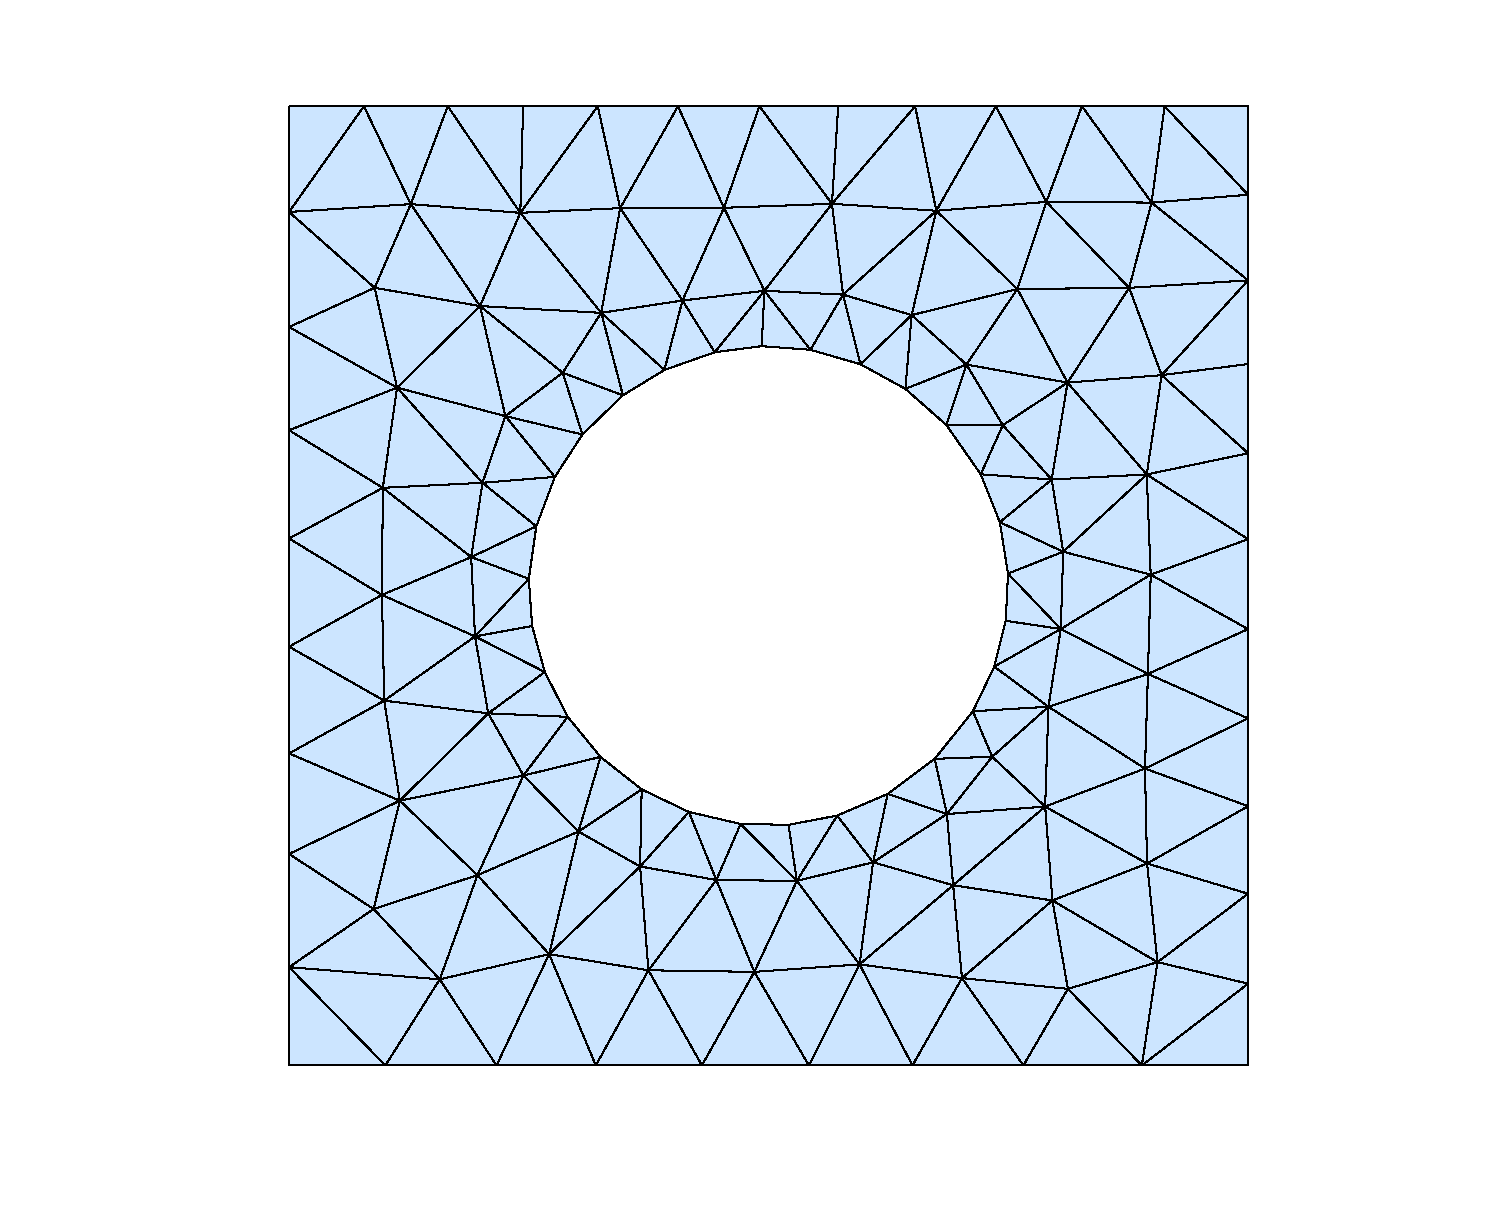
\includegraphics[width=0.9\textwidth]{usage-mesh}
\par\end{centering}

\caption{\label{fig:Mesh-distmesh}Mesh produced by \texttt{distmesh2d()}}


\end{figure}


Once the triangulation has been computed, we can create the element
type (piecewise linear\index{element!piecewise linear}):

\nwenddocs{}\nwbegincode{6}\sublabel{NWpdeB-usa7-2}\nwmargintag{{\nwtagstyle{}\subpageref{NWpdeB-usa7-2}}}\moddef{usage.m~{\nwtagstyle{}\subpageref{NWpdeB-usa7-1}}}\plusendmoddef
lin2d = lin2d_elt()
\nwendcode{}\nwbegindocs{7}\nwdocspar

The triangulation and the element type together determine the variables:

\nwenddocs{}\nwbegincode{8}\sublabel{NWpdeB-usa7-3}\nwmargintag{{\nwtagstyle{}\subpageref{NWpdeB-usa7-3}}}\moddef{usage.m~{\nwtagstyle{}\subpageref{NWpdeB-usa7-1}}}\plusendmoddef
fht = create_fht(p,t,lin2d)
nv = fht_num_vars(fht)
\nwendcode{}\nwbegindocs{9}\nwdocspar

Here \texttt{\index{fht}fht} is the geometric feature hash table,
which relates geometric features (triangles, edges, vertices) with
variable indexes. The value of \texttt{nv} is the number of variables
in the system.

Since the weak form of the PDE is
\[
\int_{\Omega}\left[\frac{\partial u}{\partial x_{1}}\frac{\partial v}{\partial x_{1}}+\frac{\partial u}{\partial x_{2}}\frac{\partial v}{\partial x_{2}}\right]d\mathbf{x}=\int_{\Omega}f(\mathbf{x})\, v(\mathbf{x})\, d\mathbf{x}
\]
where $v=0$ on $\partial\Omega$, the PDE structure representing
this for $f(\mathbf{x})=10x_{1}^{2}\exp(x_{2})$ is\index{PDE representation}

\nwenddocs{}\nwbegincode{10}\sublabel{NWpdeB-usa7-4}\nwmargintag{{\nwtagstyle{}\subpageref{NWpdeB-usa7-4}}}\moddef{usage.m~{\nwtagstyle{}\subpageref{NWpdeB-usa7-1}}}\plusendmoddef
f = @(x)(10*x(1)^2*exp(x(2)))
pde = struct('coeffs',@(x)diag([0,1,1]),'rhs',@(x)[f(x);0;0],'order',1)
\nwendcode{}\nwbegindocs{11}\nwdocspar

The \texttt{\index{coeffs}coeffs} component is a function returning
a matrix that represents the bilinear weak form above:
\[
\frac{\partial u}{\partial x_{1}}\frac{\partial v}{\partial x_{1}}+\frac{\partial u}{\partial x_{2}}\frac{\partial v}{\partial x_{2}}=\left[\begin{array}{c}
v\\
\partial v/\partial x_{1}\\
\partial v/\partial x_{2}
\end{array}\right]^{T}\left[\begin{array}{ccc}
0 & 0 & 0\\
0 & 1 & 0\\
0 & 0 & 1
\end{array}\right]\left[\begin{array}{c}
u\\
\partial u/\partial x_{1}\\
\partial u/\partial x_{2}
\end{array}\right].
\]
The \texttt{\index{rhs}rhs} component is a function returning a vector
that represents the linear part of the weak form (on the right):
\[
f(\mathbf{x})\, v(\mathbf{x})=\left[\begin{array}{c}
v(\mathbf{x})\\
\partial v/\partial x_{1}(\mathbf{x})\\
\partial v/\partial x_{2}(\mathbf{x})
\end{array}\right]^{T}\left[\begin{array}{c}
f(\mathbf{x})\\
0\\
0
\end{array}\right].
\]
The \texttt{order} component is set to one to indicate that only function
values and first order derivatives are needed. The maximum value of
\texttt{order} (in the current code) is two.

Now we need to create the matrix and right-hand side vector for the
linear system to solve. First we assemble the matrix and right-hand
side vector for the PDE. As yet, this does not deal with boundary
values: 

\nwenddocs{}\nwbegincode{12}\sublabel{NWpdeB-usa7-5}\nwmargintag{{\nwtagstyle{}\subpageref{NWpdeB-usa7-5}}}\moddef{usage.m~{\nwtagstyle{}\subpageref{NWpdeB-usa7-1}}}\plusendmoddef
% Initialize A and b 
A = sparse(nv,nv); 
b = zeros(nv,1); 
% Assemble matrix and vector  
[A,b] = assembly2d(A,b,pde,lin2d,p,t,fht,@int2d_radon7); 
\nwendcode{}\nwbegindocs{13}\nwdocspar

Note that the matrix $A$ is created as a sparse matrix. It is not
necessary to do so, but it is recommended as the systems created are
generally very sparse. The vector $\mathbf{b}$ does not need to be
created as a sparse vector. These are initialized to zero by the \texttt{sparse()}
and \texttt{zeros()} functions. The \texttt{assembly2d()} \index{assembly2d()@\texttt{assembly2d()}}function
adds the assembled matrices and vectors to the pre-existing $A$ and
$\mathbf{b}$; this feature is useful if you are combining several
different partial differential operators into one. An integration
method needed to be selected: Radon's 7-point scheme for triangles
is 5th order accurate, which is sufficient for our purposes.

Since we have \index{Dirichlet boundary conditions}Dirichlet boundary
conditions, we need to explicitly set the values of the variables
of the boundary nodes according to $g(\mathbf{x})$. First we need
to identify the boundary edges and nodes:

\nwenddocs{}\nwbegincode{14}\sublabel{NWpdeB-usa7-6}\nwmargintag{{\nwtagstyle{}\subpageref{NWpdeB-usa7-6}}}\moddef{usage.m~{\nwtagstyle{}\subpageref{NWpdeB-usa7-1}}}\plusendmoddef
[bedges,bnodes,t_index] = boundary2d(t);
\nwendcode{}\nwbegindocs{15}\nwdocspar

There are several ways of setting boundary values. The method presented
here essentially solves a least squares problem to find the finite
element function that best approximates the given $g(\mathbf{x})$.
This shows another usage of the PDE data structure\index{pde@\texttt{pde}}
as well as the boundary assembly function for $g(\mathbf{x})=\cos(x_{1})\, x_{2}$:

\nwenddocs{}\nwbegincode{16}\sublabel{NWpdeB-usa7-7}\nwmargintag{{\nwtagstyle{}\subpageref{NWpdeB-usa7-7}}}\moddef{usage.m~{\nwtagstyle{}\subpageref{NWpdeB-usa7-1}}}\plusendmoddef
g = @(x)(cos(x(1))*x(2))
pde2 = struct('coeffs',@(x)[1],'rhs',@(x)g(x),'order',0)
\nwendcode{}\nwbegindocs{17}\nwdocspar

Note that the \texttt{order} \index{order@\texttt{order}}parameter
is set to zero to indicate that no derivatives are involved. Then
we assemble the normal equations matrix and right-hand side for the
least squares problem:

\nwenddocs{}\nwbegincode{18}\sublabel{NWpdeB-usa7-8}\nwmargintag{{\nwtagstyle{}\subpageref{NWpdeB-usa7-8}}}\moddef{usage.m~{\nwtagstyle{}\subpageref{NWpdeB-usa7-1}}}\plusendmoddef
[Ab,bb,bvlist] = assembly2dbdry(pde2,lin2d,p,t,bedges,t_index,fht,@int1d_gauss5);
\nwendcode{}\nwbegindocs{19}\nwdocspar

Now we solve the linear system to obtain values of the boundary variables.

\nwenddocs{}\nwbegincode{20}\sublabel{NWpdeB-usa7-9}\nwmargintag{{\nwtagstyle{}\subpageref{NWpdeB-usa7-9}}}\moddef{usage.m~{\nwtagstyle{}\subpageref{NWpdeB-usa7-1}}}\plusendmoddef
g1 = Ab(bvlist,bvlist) \\ bb(bvlist);
\nwendcode{}\nwbegindocs{21}\nwdocspar

Now we can solve the remainder of the system for the non-boundary
variables. First, find the non-boundary variables (\texttt{cbvlist}
means ``complement of \texttt{bvlist}'').

\nwenddocs{}\nwbegincode{22}\sublabel{NWpdeB-usa7-A}\nwmargintag{{\nwtagstyle{}\subpageref{NWpdeB-usa7-A}}}\moddef{usage.m~{\nwtagstyle{}\subpageref{NWpdeB-usa7-1}}}\plusendmoddef
% find non-boundary variables (cbvlist) 
v_array = ones(nv,1); v_array(bvlist) = 0; 
cbvlist = find(v_array ~= 0);

\nwendcode{}\nwbegindocs{23}\nwdocspar

Now we solve the linear system for the non-boundary variables and
insert the results into the vector $\mathbf{u}$; the boundary variables
in $\mathbf{u}$ are in \texttt{g1}. 

\nwenddocs{}\nwbegincode{24}\sublabel{NWpdeB-usa7-B}\nwmargintag{{\nwtagstyle{}\subpageref{NWpdeB-usa7-B}}}\moddef{usage.m~{\nwtagstyle{}\subpageref{NWpdeB-usa7-1}}}\plusendmoddef
u_int = A(cbvlist,cbvlist) \\ (b(cbvlist) - A(cbvlist,bvlist)*g1);
u = zeros(nv,1); 
u(cbvlist) = u_int; 
u( bvlist) = g1; 

\nwendcode{}\nwbegindocs{25}\nwdocspar

We can plot the values of our numerical solution $u(\mathbf{x})$
at the vertices of the triangulation by means of \texttt{\index{trimesh()}trimesh()}
and a helper routine \texttt{\index{pvlist()}pvlist()} that returns
the variable indexes for the vertices of the triangulation.

\nwenddocs{}\nwbegincode{26}\sublabel{NWpdeB-usa7-C}\nwmargintag{{\nwtagstyle{}\subpageref{NWpdeB-usa7-C}}}\moddef{usage.m~{\nwtagstyle{}\subpageref{NWpdeB-usa7-1}}}\plusendmoddef
pvlist = get_pvlist(fht,np); 
figure(2)
trimesh(t,p(:,1),p(:,2),u(pvlist))

\nwendcode{}\nwbegindocs{27}\nwdocspar

The result is illustrated in Figure~\ref{fig:Computed-solution1}.

\begin{figure}
\noindent \begin{centering}
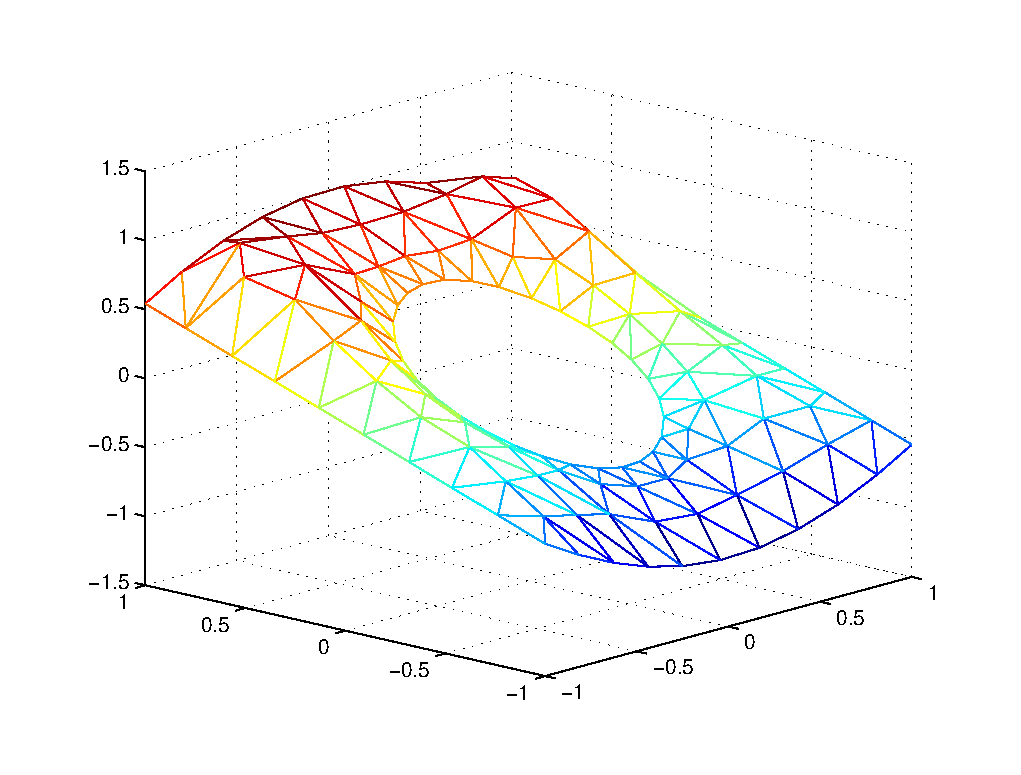
\includegraphics[width=0.9\textwidth]{usage-soln1}
\par\end{centering}

\caption{\label{fig:Computed-solution1}Computed solution to PDE}


\end{figure}


To repeat the calculation using piecewise quadratic elements, we must
first create the associated element type structure, and create the
feature hash table for that element type.\index{element!piecewise quadratic}\index{quad2d_elt()@\texttt{quad2d\_elt()}}

\nwenddocs{}\nwbegincode{28}\sublabel{NWpdeB-usa7-D}\nwmargintag{{\nwtagstyle{}\subpageref{NWpdeB-usa7-D}}}\moddef{usage.m~{\nwtagstyle{}\subpageref{NWpdeB-usa7-1}}}\plusendmoddef
% Now using piecewise quadratic elements
quad2d = quad2d_elt()
fht2 = create_fht(p,t,quad2d)
nv2 = fht_num_vars(fht2)
\nwendcode{}\nwbegindocs{29}\nwdocspar

Then we need to assemble the matrix and right-hand side:\index{assembly2d()@\texttt{assembly2d()}}

\nwenddocs{}\nwbegincode{30}\sublabel{NWpdeB-usa7-E}\nwmargintag{{\nwtagstyle{}\subpageref{NWpdeB-usa7-E}}}\moddef{usage.m~{\nwtagstyle{}\subpageref{NWpdeB-usa7-1}}}\plusendmoddef
% Initialize A2 and b2 
A2 = sparse(nv2,nv2); 
b2 = zeros(nv2,1); 
% Assemble matrix and vector  
[A2,b2] = assembly2d(A2,b2,pde,quad2d,p,t,fht2,@int2d_radon7); 
\nwendcode{}\nwbegindocs{31}\nwdocspar

Note that the \texttt{\index{pde}pde} structure remains unchanged,
as does the triangulation. While the boundary nodes remain unchanged,
the boundary \emph{variables} do not. We also use the least-squares
approach to the Dirichlet boundary values, which works just as well
for the case of piecewise quadratic elements as for piecewise linear
elements. So we use the following code:

\nwenddocs{}\nwbegincode{32}\sublabel{NWpdeB-usa7-F}\nwmargintag{{\nwtagstyle{}\subpageref{NWpdeB-usa7-F}}}\moddef{usage.m~{\nwtagstyle{}\subpageref{NWpdeB-usa7-1}}}\plusendmoddef
[Ab2,bb2,bvlist2] = ...
    assembly2dbdry(pde2,quad2d,p,t,bedges,t_index,fht2,@int1d_gauss5);
% find non-boundary variables (cbvlist2) 
v_array = ones(nv2,1); v_array(bvlist2) = 0; 
cbvlist2 = find(v_array ~= 0);

g2 = Ab2(bvlist2,bvlist2) \\ bb2(bvlist2);
u_int = A2(cbvlist2,cbvlist2) \\ (b2(cbvlist2) - A2(cbvlist2,bvlist2)*g2);
u2 = zeros(nv2,1); 
u2(cbvlist2) = u_int; 
u2( bvlist2) = g2; 
\nwendcode{}\nwbegindocs{33}\nwdocspar

To properly display the results, which are more accurate than the
results of piecewise linear elements, we should use sub-meshes. First
we create the sub-mesh for the \index{reference element}reference
element (which is the triangle with vertices $(0,0)$, $(1,0)$, and
$(0,1)$):

\nwenddocs{}\nwbegincode{34}\sublabel{NWpdeB-usa7-G}\nwmargintag{{\nwtagstyle{}\subpageref{NWpdeB-usa7-G}}}\moddef{usage.m~{\nwtagstyle{}\subpageref{NWpdeB-usa7-1}}}\plusendmoddef
[pr,tr] = ref_triangle_submesh(4);
\nwendcode{}\nwbegindocs{35}\nwdocspar

The returned triangulation of the reference element has the edges
of 4 small triangles on each coordinate axis. Then we can generate
the values on a sub-mesh of the original triangulation, and plot the
results.

\nwenddocs{}\nwbegincode{36}\sublabel{NWpdeB-usa7-H}\nwmargintag{{\nwtagstyle{}\subpageref{NWpdeB-usa7-H}}}\moddef{usage.m~{\nwtagstyle{}\subpageref{NWpdeB-usa7-1}}}\plusendmoddef
[pv,tv,vals] = get_submesh_vals(p,t,fht2,quad2d,u2,pr,tr,0);
figure(3)
trimesh(tv,pv(:,1),pv(:,2),vals)
\nwendcode{}\nwbegindocs{37}\nwdocspar

The last input to \texttt{get\_submesh\_vals()} is the maximum order
of the derivatives values generated. Since we just want to plot the
values of the solution, this is set to zero. The result is shown in
Figure~\ref{fig:Results-quadratic-elt}.

\begin{figure}
\noindent \begin{centering}
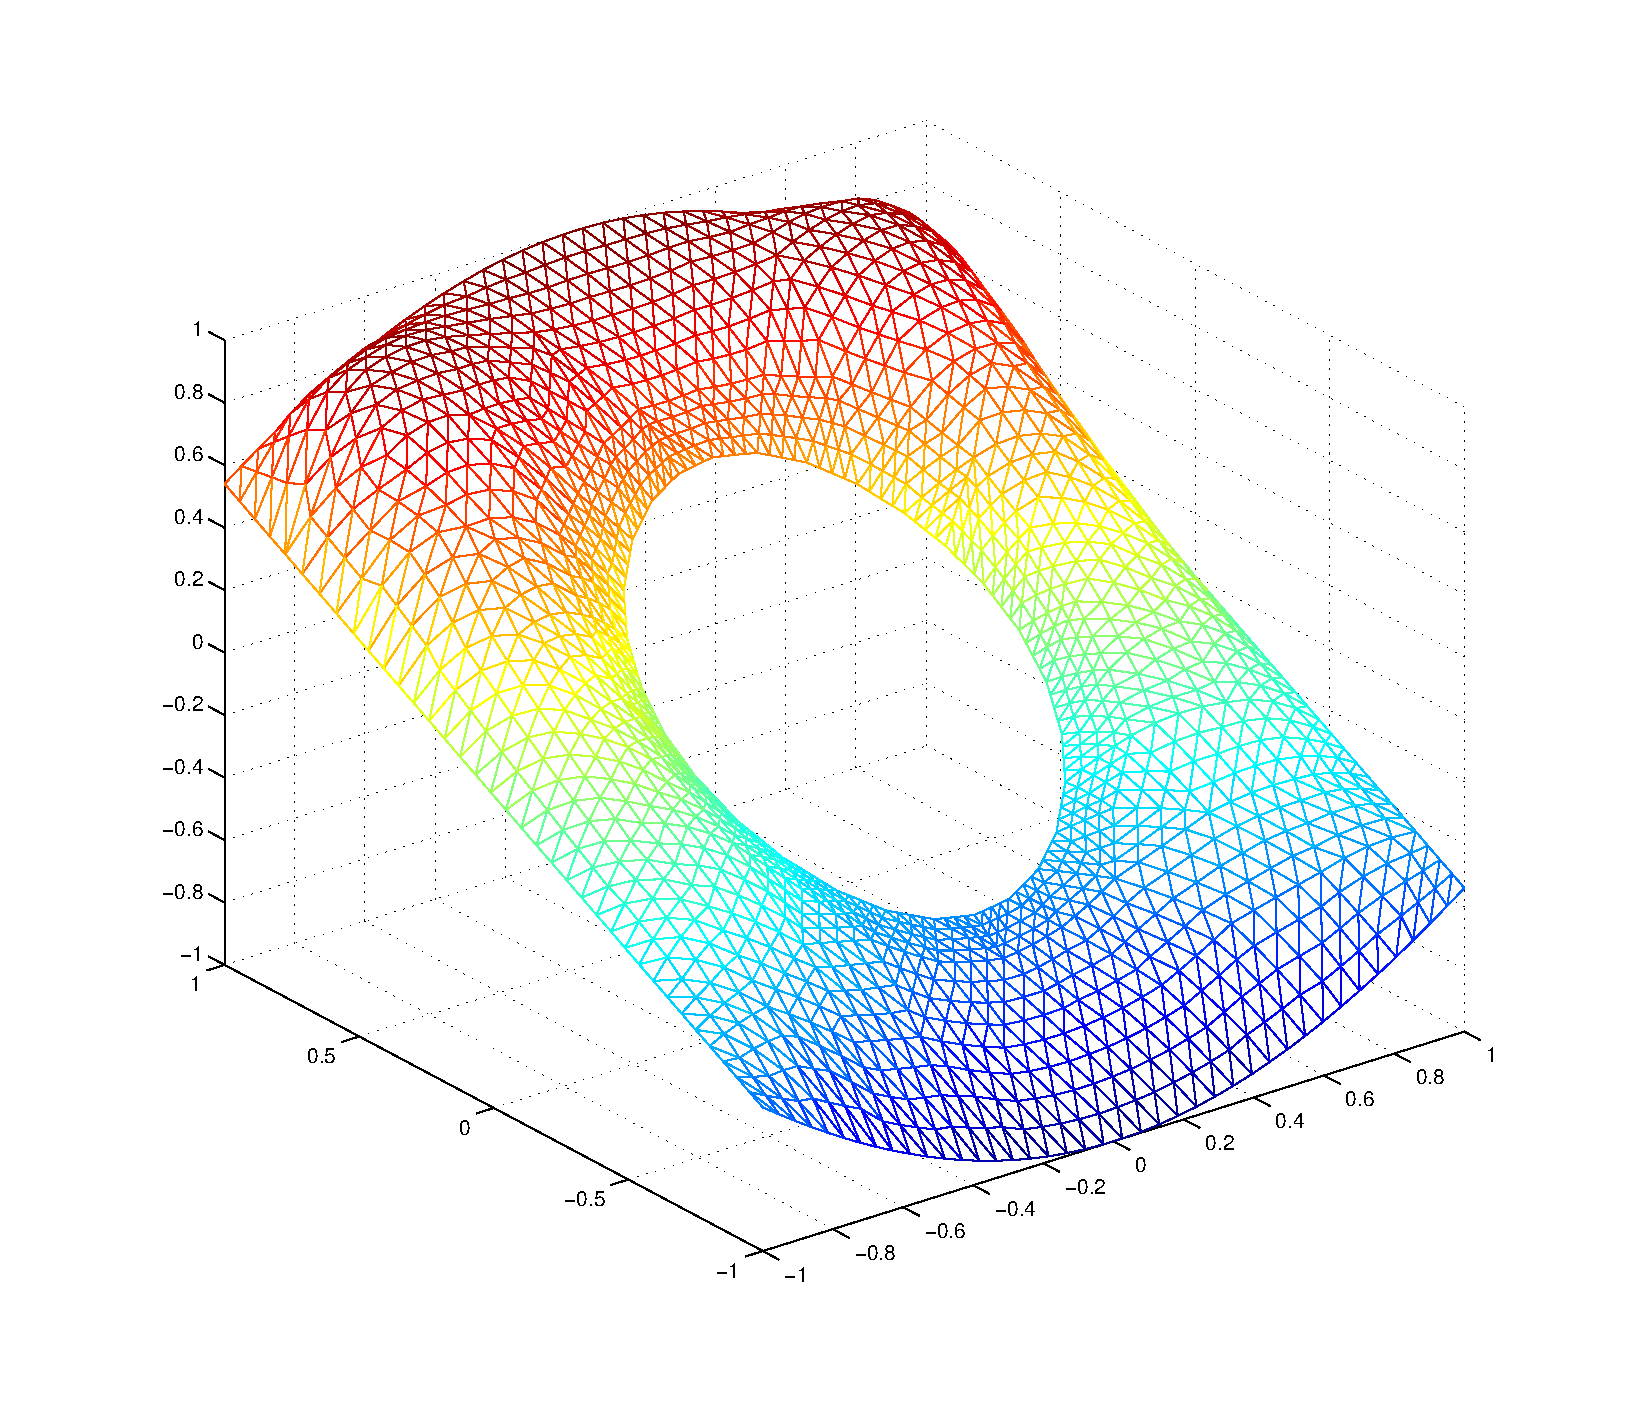
\includegraphics[width=0.9\textwidth]{usage-soln2}
\par\end{centering}

\caption{\label{fig:Results-quadratic-elt}Results of using quadratic elements
(plotted using a sub-mesh)}


\end{figure}



\subsubsection{Usage: a convection diffusion problem}

\index{convection--diffusion problem}This equation is more complex
than the previous example, but on the same region:
\begin{eqnarray*}
-\nabla\cdot\left[\alpha(\mathbf{x})\nabla u\right]+\mathbf{w}(\mathbf{x})\cdot\nabla u & = & f(\mathbf{x})\qquad\mbox{in }\Omega,\\
u(\mathbf{x}) & = & g(\mathbf{x})\qquad\mbox{on }\Gamma_{1},\\
\beta(\mathbf{x})u(\mathbf{x})+\alpha(\mathbf{x})\frac{\partial u}{\partial n}(\mathbf{x}) & = & h(\mathbf{x})\qquad\mbox{on }\Gamma_{2},
\end{eqnarray*}
where $\Gamma_{1}$ is the outer boundary, and $\Gamma_{2}$ is the
inner (circular) boundary. The boundary conditions over $\Gamma_{2}$
are called \index{Robin boundary conditions}Robin boundary conditions.
In the case where $\beta(\mathbf{x})\equiv0$, they are called \index{Neumann boundary conditions}Neumann
boundary conditions, or \index{natural boundary conditions}natural
boundary conditions. To obtain the weak form, multiply by a function
$v(\mathbf{x})$ with $v=0$ on $\Gamma_{1}$ and integrate over $\Omega$:
\[
\int_{\Omega}v\left(-\nabla\cdot\left[\alpha(\mathbf{x})\nabla u\right]+\mathbf{w}(\mathbf{x})\cdot\nabla u\right)d\mathbf{x}=\int_{\Omega}v\, f\, d\mathbf{x}.
\]
The left-hand side can be re-arranged using
\begin{eqnarray*}
\int_{\Omega}v\nabla\cdot\left[\alpha\nabla u\right]\, d\mathbf{x} & = & \int_{\Omega}\left\{ \nabla\cdot\left(v\alpha\nabla u\right)-\alpha\nabla v\cdot\nabla u\right\} \, d\mathbf{x}\\
 & = & \int_{\partial\Omega}v\alpha\frac{\partial u}{\partial n}\, dS-\int_{\Omega}\alpha\nabla v\cdot\nabla u\, d\mathbf{x}\\
 & = & \int_{\Gamma_{2}}v\alpha\frac{\partial u}{\partial n}\, dS-\int_{\Omega}\alpha\nabla v\cdot\nabla u\, d\mathbf{x}
\end{eqnarray*}
since $v=0$ on $\Gamma_{1}$ , $\overline{\Gamma_{1}}\cup\overline{\Gamma_{2}}=\partial\Omega$,
and $\Gamma_{1}\cap\Gamma_{2}=\emptyset$. Now we can use the boundary
conditions on $\Gamma_{2}$:
\begin{eqnarray*}
\int_{\Gamma_{2}}v\alpha\frac{\partial u}{\partial n}\, dS & = & \int_{\Gamma_{2}}v\left[h-\beta u\right]\, dS.
\end{eqnarray*}
Combining, this gives the weak form
\[
\int_{\Omega}\left[\alpha\nabla v\cdot\nabla u+v\,\mathbf{w}\cdot\nabla u\right]d\mathbf{x}+\int_{\Gamma_{2}}\beta uv\, dS=\int_{\Omega}f\, v\, d\mathbf{x}+\int_{\Gamma_{2}}h\, v\, dS,
\]
for all $v$ with $v=0$ on $\Gamma_{1}$, and $u=g$ on $\Gamma_{1}$.

We need to define the \texttt{pde} structures for the region and boundary
integrals. 

\nwenddocs{}\nwbegincode{38}\sublabel{NWpdeB-usa7-I}\nwmargintag{{\nwtagstyle{}\subpageref{NWpdeB-usa7-I}}}\moddef{usage.m~{\nwtagstyle{}\subpageref{NWpdeB-usa7-1}}}\plusendmoddef
f = @(x)10;
%g = @(x)(0.5*cos(x(1)));
g = @(x)0;
h = @(x)exp(x(2));
w = @(x)[1; -2];
alpha = @(x)1;
beta  = @(x)10;
pde  = struct('coeffs',@(x)[0,w(x)'; [0;0],alpha(x)*eye(2)], ...
         'rhs',@(x)[f(x);0;0], 'order',1)
pdeb = struct('coeffs',beta, 'rhs',h, 'order',0)

\nwendcode{}\nwbegindocs{39}\nwdocspar

Note that $f(\mathbf{x})$, $\mathbf{w}(\mathbf{x})$, and $\alpha(\mathbf{x})$
are only evaluated once for each value of $\mathbf{x}$. 

We also need to separate out the edges on $\Gamma_{1}$ and $\Gamma_{2}$.
A simple way to separate them is that points $\mathbf{x}$ on $\Gamma_{1}$
have $\left\Vert \mathbf{x}\right\Vert _{2}>3/4$ while points $\mathbf{x}$
on $\Gamma_{2}$ have $\left\Vert \mathbf{x}\right\Vert _{2}<3/4$.
Fortunately in this case, there are no edges that intersect both $\Gamma_{1}$
and $\Gamma_{2}$, although this may occur with other problems. 

This task can be carried by starting with \texttt{\index{bnodes}bnodes},
which contains the list of boundary vertices as indexes into the \texttt{p}
array. 

\nwenddocs{}\nwbegincode{40}\sublabel{NWpdeB-usa7-J}\nwmargintag{{\nwtagstyle{}\subpageref{NWpdeB-usa7-J}}}\moddef{usage.m~{\nwtagstyle{}\subpageref{NWpdeB-usa7-1}}}\plusendmoddef
in_gamma1_bnodes = (sqrt(p(bnodes,1).^2+p(bnodes,2).^2) > 3/4);
\nwendcode{}\nwbegindocs{41}\nwdocspar

Note that \texttt{in\_gamma1\_bnodes(i)} is true (1) or false (0)
depending on whether the point indexed by \texttt{bnodes(i)} is in
$\Gamma_{1}$. We create a boolean (that is, zero--one) vector indicating
whether a given point of the triangulation is in $\Gamma_{1}$:

\nwenddocs{}\nwbegincode{42}\sublabel{NWpdeB-usa7-K}\nwmargintag{{\nwtagstyle{}\subpageref{NWpdeB-usa7-K}}}\moddef{usage.m~{\nwtagstyle{}\subpageref{NWpdeB-usa7-1}}}\plusendmoddef
in_gamma1 = zeros(size(p,1),1);
in_gamma1(bnodes) = in_gamma1_bnodes;
\nwendcode{}\nwbegindocs{43}\nwdocspar

Then we can check the boundary edges to see which boundary edges are
in $\Gamma_{1}$:

\nwenddocs{}\nwbegincode{44}\sublabel{NWpdeB-usa7-L}\nwmargintag{{\nwtagstyle{}\subpageref{NWpdeB-usa7-L}}}\moddef{usage.m~{\nwtagstyle{}\subpageref{NWpdeB-usa7-1}}}\plusendmoddef
in_gamma1_bedges = in_gamma1(bedges(:,1)) & in_gamma1(bedges(:,2));
bedges1  = bedges (find( in_gamma1_bedges),:);
t_index1 = t_index(find( in_gamma1_bedges));
bedges2  = bedges (find(~in_gamma1_bedges),:);
t_index2 = t_index(find(~in_gamma1_bedges));
\nwendcode{}\nwbegindocs{45}\nwdocspar

The boundaries can be shown by means of the \texttt{triplot()} function:

\nwenddocs{}\nwbegincode{46}\sublabel{NWpdeB-usa7-M}\nwmargintag{{\nwtagstyle{}\subpageref{NWpdeB-usa7-M}}}\moddef{usage.m~{\nwtagstyle{}\subpageref{NWpdeB-usa7-1}}}\plusendmoddef
figure(4)
triplot(t,p(:,1),p(:,2),'k') % plot triangulation
% plot \\Gamma_1 in blue and \\Gamma_2 in red
triplot([bedges1(:,1),bedges1(:,2),bedges1(:,2)],p(:,1),p(:,2),'b')
triplot([bedges2(:,1),bedges2(:,2),bedges2(:,2)],p(:,1),p(:,2),'r')
\nwendcode{}\nwbegindocs{47}\nwdocspar

The result is shown in Figure~\ref{fig:two-boundaries}.

\begin{figure}
\noindent \begin{centering}
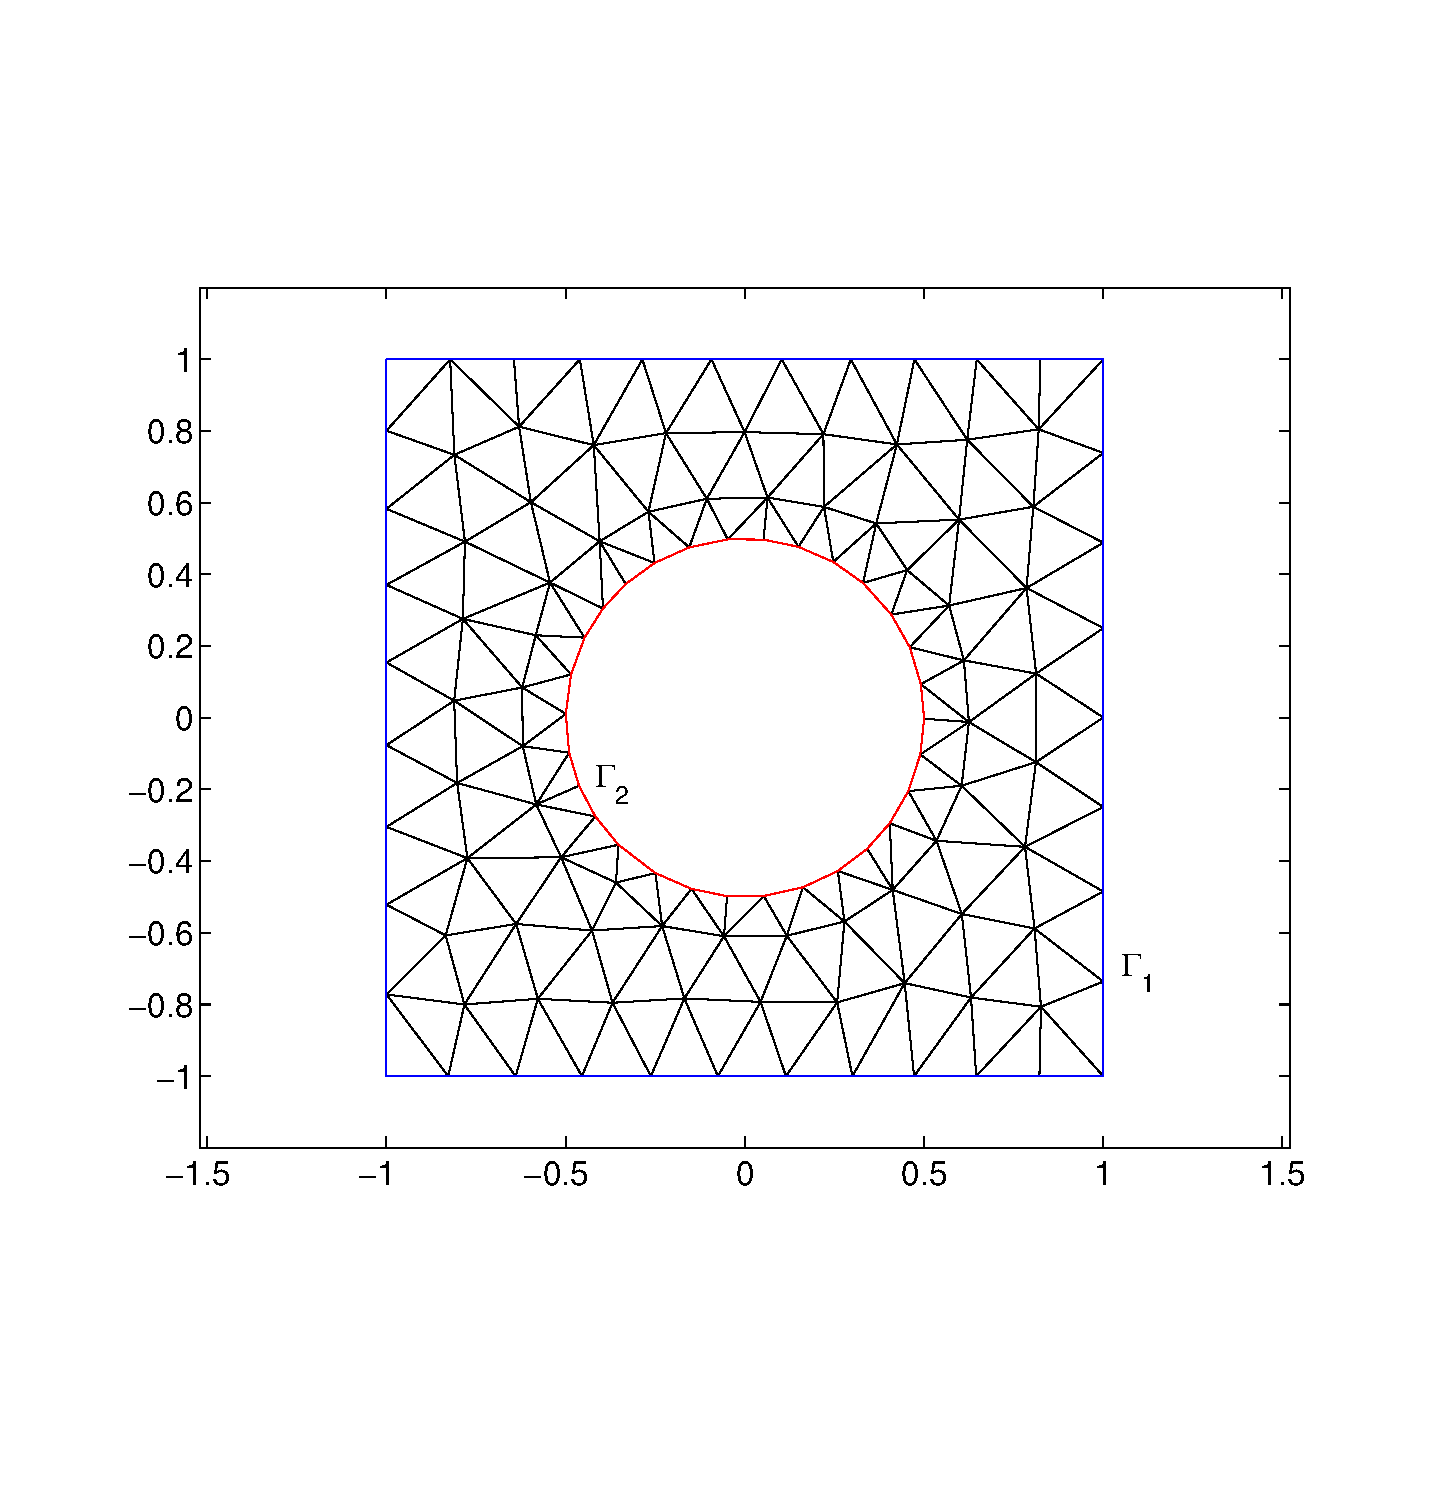
\includegraphics[width=0.9\textwidth]{two-boundaries}
\par\end{centering}

\caption{\label{fig:two-boundaries}Boundaries $\Gamma_{1}$ and $\Gamma_{2}$ }


\end{figure}


Then to create the linear system to solve, we need to find all the
variables associated with the Dirichlet boundary conditions; that
is, we need to find all variables associated with $\Gamma_{1}$. The
main matrix and right-hand side can be assembled independently. 

\nwenddocs{}\nwbegincode{48}\sublabel{NWpdeB-usa7-N}\nwmargintag{{\nwtagstyle{}\subpageref{NWpdeB-usa7-N}}}\moddef{usage.m~{\nwtagstyle{}\subpageref{NWpdeB-usa7-1}}}\plusendmoddef
intmethod = @int2d_radon7;
[A,b,bvlist2] = assembly2dbdry(pdeb,lin2d,p,t, ...
      bedges2,t_index2,fht,@int1d_gauss5);
[A,b] = assembly2d(A,b,pde,lin2d,p,t,fht,intmethod);
dir_bc_pde = struct('coeffs',@(x)[1],'rhs',@(x)g(x),'order',0)
Ab = sparse(nv,nv);
bb =  zeros(nv,1);
[Ab,bb,dir_bc_vlist] = ... 
      assembly2dbdry(dir_bc_pde,lin2d,p,t, ...
      bedges1,t_index1,fht,@int1d_gauss5);
u1 = Ab(dir_bc_vlist,dir_bc_vlist) \\ bb(dir_bc_vlist);
% Get complement to dir_bc_vlist
varray = zeros(nv,1);
varray(dir_bc_vlist) = 1;
cvlist = find(varray == 0);
% Now solve linear system
u2 = A(cvlist,cvlist) \\ (b(cvlist) - A(cvlist,dir_bc_vlist)*u1);
u = zeros(nv,1);
u(dir_bc_vlist) = u1;
u(cvlist)       = u2;
figure(5)
trimesh(t,p(:,1),p(:,2),u(pvlist))
\nwendcode{}\nwbegindocs{49}\nwdocspar

The result is shown in Figure~\ref{fig:convection-diffusion-robin-bc}.

\begin{figure}
\noindent \begin{centering}
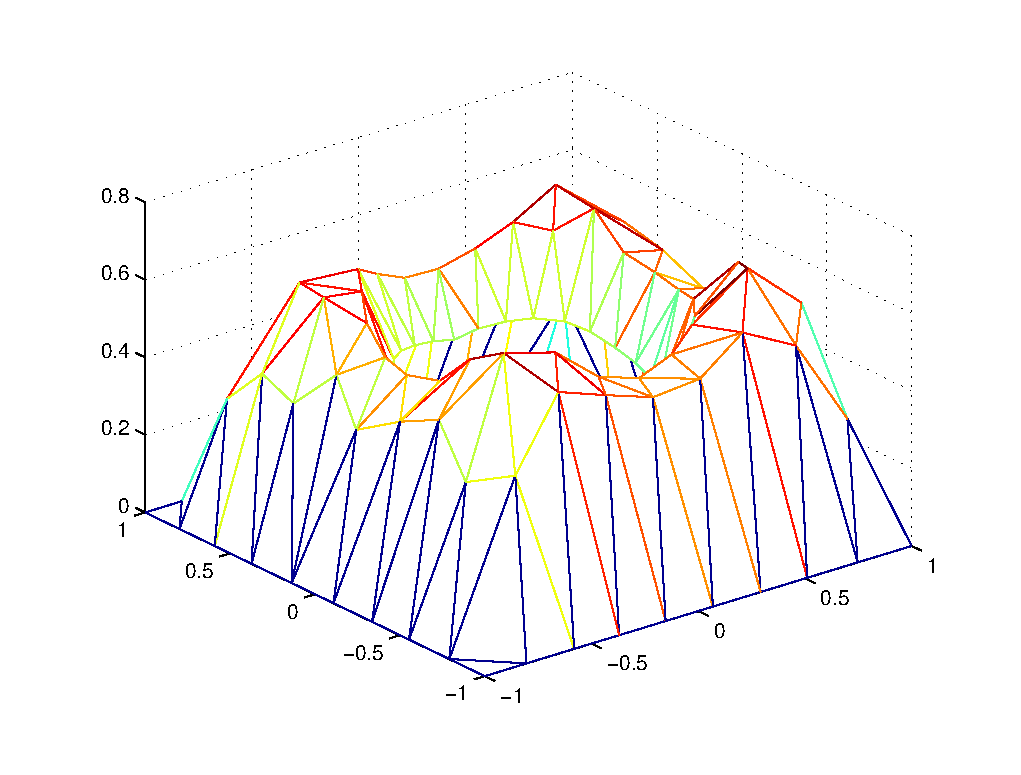
\includegraphics[width=0.9\textwidth]{conv-diff-eg}
\par\end{centering}

\caption{\label{fig:convection-diffusion-robin-bc}Result for convection--diffusion
problem with Robin boundary conditions}


\end{figure}



\section{\label{sec:Basic-assumptions}Basic assumptions}

There are a number of assumptions about the triangulation and the
element types (which includes their basis functions) that are necessary
for this code to work. It is important to be aware of these issues
when, for example, creating new element types, or using different
mesh generators.

The triangulation is represented by the pair of arrays (\texttt{p},\texttt{t})
where rows of \texttt{p} are the $(x,y)$ co-ordinates of the vertices
(points) of the triangulation, and each row of \texttt{t} contains
the row indexes into \texttt{p} for the vertices of that triangle.
Thus \texttt{p} is a floating point array with two columns and \texttt{t}
is an integer array with three columns. For three-dimensions, \texttt{p}
is a floating point array with three columns (for $x$, $y$ and $z$
coordinates) and \texttt{t} is an integer array with four columns
representing the vertices of tetrahedra.

The triangulation is assumed to be \emph{conforming}. That is, for
any two triangles $K_{1}$ and $K_{2}$ in the triangulation, $K_{1}\cap K_{2}$
is either empty, or a common \emph{geometric feature} (vertex, edge,
or triangle). Vertices are represented by a single row index into
\texttt{p}, edges by a pair of row indexes into \texttt{p}, and triangles
by three row indexes into \texttt{p}.

Each triangle $K$ in the triangulation has a number of associated
basis functions $\phi_{i}(\mathbf{x})$. These are basis functions
are related to basis functions on the \emph{reference element} $\widehat{K}$.
For this code, the reference element is the triangle with vertices
$(0,0)$, $(1,0)$, and $(0,1)$. The basis functions on the reference
element are fixed functions $\widehat{\phi}_{j}(\widehat{\mathbf{x}})$
for $\widehat{\mathbf{x}}\in\widehat{K}$. Each triangle $K$ in the
triangulation is the image of the reference element under an affine
transformation $\widehat{K}\to K$ given by $\widehat{\mathbf{x}}\mapsto\mathbf{x}=T_{K}\widehat{\mathbf{x}}+\mathbf{b}_{K}$.
Then each basis function $\phi_{i}$ that is non-zero on $K$ is related
to some basis function $\widehat{\phi}_{j}$ on $\widehat{K}$ through
$\phi_{i}(\mathbf{x})=\widehat{\phi}_{j}(\widehat{\mathbf{x}})$ where
$\mathbf{x}=T_{K}\widehat{\mathbf{x}}+\mathbf{b}_{K}$. (This requirement
is actually relaxed for some element types to requiring that $\phi_{i}(\mathbf{x})=\sum_{j}c_{ij}\,\widehat{\phi}_{j}(\widehat{\mathbf{x}})$
for some linear combination of basis functions on the reference element.)

Every basis function (or variable) on the reference element is associated
with a unique geometric feature of the reference element. If $\widehat{\mathbf{x}}$
belongs to a geometric feature and $\widehat{\phi}_{j}$ is \emph{not}
associated with that geometric feature or any of its subfeatures,
then $\widehat{\phi}_{j}(\widehat{\mathbf{x}})=0$ if the basis functions
are continuous across element boundaries. Piecewise constant elements
are not continuous across element boundaries, and so do not have to
satisfy this requirement.

Any permutation of the vertices of the reference triangle $\widehat{K}$
induces an affine transformation $\widehat{K}\to\widehat{K}$ given
by $\widehat{\mathbf{x}}\mapsto\widehat{T}\widehat{\mathbf{x}}+\widehat{\mathbf{b}}$.
For each basis function $\widehat{\phi}_{j}$ and permutation of the
vertices of $\widehat{K}$, $\widehat{\mathbf{x}}\mapsto\widehat{\phi}_{j}(\widehat{T}\widehat{\mathbf{x}}+\widehat{\mathbf{b}})$
is a $\widehat{\phi}_{k}$ basis functions. That is, for some coefficients
$c_{k}$,
\[
\widehat{\phi}_{j}(\widehat{T}\widehat{\mathbf{x}}+\widehat{\mathbf{b}})=\sum_{k}c_{k}\,\widehat{\phi}_{k}(\widehat{\mathbf{x}})\qquad\mbox{for all }\widehat{\mathbf{x}}\in\widehat{K}.
\]


Very often we can write $\widehat{\phi}_{j}(\widehat{T}\widehat{\mathbf{x}}+\widehat{\mathbf{b}})=\widehat{\phi}_{k}(\widehat{\mathbf{x}})$
for all $\widehat{\mathbf{x}}\in\widehat{K}$ for some $k$. For example,
consider the piecewise linear, quadratic and cubic Lagrange elements:
using a nodal basis with nodes that are symmetrically placed with
respect to permutations of the vertices means that $\widehat{\phi}_{j}(\widehat{T}\widehat{\mathbf{x}}+\widehat{\mathbf{b}})=\widehat{\phi}_{k}(\widehat{\mathbf{x}})$
for some $k$.


\section{\label{sec:Matrix-assembly-code}Matrix assembly code}

The main matrix assembly code \texttt{\index{assembly2d()}assembly2d()}
is given below. The function adds values in the matrix $A$ and the
vector $\mathbf{b}$. In this way, the full assembly process can be
accomplished ``in pieces'', if needed. So, for stand-alone use,
$A$ and $\mathbf{b}$ must be initialized to zero. Note that $A$
can (and should) be a sparse matrix.

The PDE is represented by two functions which are in the \texttt{pde}
structure (see Subsection~\ref{sub:PDE-representation}).

The element type is defined by the \texttt{\index{elt}elt} structure
(see Section~\ref{sec:Element-types}).

The triangulation is given by the pair (\texttt{p},\texttt{t}) as
described in Section~\ref{sec:Overview}. 

The hash table for the map from geometric features (triangles, edges,
and vertices) to variables is \texttt{\index{fht}fht} (see Section~\ref{sec:Handling-geometric-features}).

The points and weights for the integration method on the reference
element are returned by the function \texttt{intmethod()} (see Section~\ref{sec:Numerical-integration}).
These points and weights are computed in \emph{assembly2d-init}.

The line
\begin{lyxcode}
{[}vlist,slist{]}~=~get\_var\_triangle(t(i,:),fht,elt,np);
\end{lyxcode}
gets the list of (global) variables indexes (\texttt{vlist}) associated
with triangle $i$, along with the list of sign changes needed (\texttt{slist}). 


\subsection{Main two-dimensional assembly function}

\nwenddocs{}\nwbegincode{50}\sublabel{NWpdeB-fil8-2}\nwmargintag{{\nwtagstyle{}\subpageref{NWpdeB-fil8-2}}}\moddef{filelist~{\nwtagstyle{}\subpageref{NWpdeB-fil8-1}}}\plusendmoddef
assembly2d.m \\
\nwendcode{}\nwbegincode{51}\sublabel{NWpdeB-assC-1}\nwmargintag{{\nwtagstyle{}\subpageref{NWpdeB-assC-1}}}\moddef{assembly2d.m~{\nwtagstyle{}\subpageref{NWpdeB-assC-1}}}\endmoddef
function [A,b] = assembly2d(A,b,pde,elt,p,t,fht,intmethod)
% function [A,b] = assembly2d(A,b,pde,elt,p,t,fht,intmethod)
% Adds the assembled matrix and vector representing the
% given PDE (pde) to the A matrix & b vector.
% This uses a given element (elt) with the triangulation given by (p,t).
% The feature hash table (fht) is used to obtain variable indexes
% for given features. This is obtained by create_fht().
%
% A must be nv x nv and b must be nv x 1 where nv is the total
% number of variables (as returned by fht_num_vars()).
% Reference triangle has vertices (0,0), (1,0), (0,1).
\LA{}assembly2d-init~{\nwtagstyle{}\subpageref{NWpdeB-assF-1}}\RA{}
\LA{}assembly2d-precompute-Aphihat~{\nwtagstyle{}\subpageref{NWpdeB-assT-1}}\RA{}
for i = 1:size(t,1) % for all triangles ...
    % obtain variable list and signs for this triangle
    [vlist,slist] = get_var_triangle(t(i,:),fht,elt,np);
    % set up affine transformation xhat :-> x = T.xhat + b0
    i1 = t(i,1);  i2 = t(i,2);  i3 = t(i,3);
    T = [p(i2,:)'-p(i1,:)', p(i3,:)'-p(i1,:)'];
    b0 = p(i1,:)';
    % form weighted sum of integrand at integration points
    intval1 = 0;
    intval2 = 0;
    for k = 1:length(w_int)
        Aphival = elt.trans_Aphihat(T,Aphihatvals\{k\},order);
        Dmat    = pde.coeffs(T*p_int(k,:)'+b0);
        rhsvec  = pde.rhs(T*p_int(k,:)'+b0);
        integrand_val1 = Aphival*Dmat*Aphival';
        integrand_val2 = Aphival*rhsvec;
        intval1 = intval1 + w_int(k)*integrand_val1;
        intval2 = intval2 + w_int(k)*integrand_val2;
    end
    detT = abs(det(T));
    intval1 = intval1*detT; % scale by Jacobian
    intval2 = intval2*detT;
    intval1 = diag(slist)*intval1*diag(slist); % change signs if needed
    % intval2 = slist'.*intval2;
    intval2 = bsxfun(@times,intval2,slist');
    A(vlist,vlist) = A(vlist,vlist) + intval1; % add to matrix & vec
    % b(vlist) = b(vlist) + intval2;
    b(vlist,:) = b(vlist,:) + intval2;
end
\nwnotused{assembly2d.m}\nwendcode{}\nwbegindocs{52}\nwdocspar

Initialization for \emph{assembly2d}:

\nwenddocs{}\nwbegincode{53}\sublabel{NWpdeB-assF-1}\nwmargintag{{\nwtagstyle{}\subpageref{NWpdeB-assF-1}}}\moddef{assembly2d-init~{\nwtagstyle{}\subpageref{NWpdeB-assF-1}}}\endmoddef
[p_int,w_int] = intmethod(); % points and weights for reference triangle
% np is the total number of points in the triangulation
np = size(p,1);
% compute nv = total number of variables
nv = fht_num_vars(fht);
% nv_elt is the number of variables in one element
nv_elt = sum(elt.nvars);
% order is the order of derivatives used in the assembly;
% we need 0 <= order <= 2
order = pde.order;
intval1 = zeros(nv_elt,nv_elt);
% intval2 = zero(nv_elt,1);
intval2 = zeros(nv_elt,size(b,2));
\nwused{\\{NWpdeB-assC-1}}\nwendcode{}\nwbegindocs{54}\nwdocspar

For efficiency, we precompute the values of $\mathcal{A}\widehat{\phi}_{i}(\widehat{\mathbf{x}}_{j})$
where $\widehat{\mathbf{x}}_{j}$ are the integration points on the
reference triangle. These depend only on the element type and the
reference element $\widehat{K}$. 

\nwenddocs{}\nwbegincode{55}\sublabel{NWpdeB-assT-1}\nwmargintag{{\nwtagstyle{}\subpageref{NWpdeB-assT-1}}}\moddef{assembly2d-precompute-Aphihat~{\nwtagstyle{}\subpageref{NWpdeB-assT-1}}}\endmoddef
% Save Aphihat() values for all the integration points
% on the reference element
Aphihatvals = cell(length(w_int),1);
for k = 1:length(w_int)
    Aphihatvals\{k\} = elt.Aphihat(p_int(k,:),order);
end
\nwused{\\{NWpdeB-assC-1}}\nwendcode{}\nwbegindocs{56}\nwdocspar

{}


\subsection{\label{sub:Petrov--Galerkin-method}Petrov--Galerkin method}

The Petrov--Galerkin method is supported through the \texttt{\index{pgassembly2d()}pgassembly2d()}
function. Since there are potentially two different elements used
(\texttt{elt1} and \texttt{elt2}), we need to pass two separate feature
hash tables (\texttt{fht1} and \texttt{fht2}). Otherwise the inputs
are identical to those for the standard Galerkin assembly function
\texttt{assembly2d()}. Note that \texttt{assembly2d()} is equivalent
to 
\begin{lyxcode}
pgassembly2d(A,b,pde,p,t,elt,fht,elt,fht,intmethod)
\end{lyxcode}
{}

\nwenddocs{}\nwbegincode{57}\sublabel{NWpdeB-fil8-3}\nwmargintag{{\nwtagstyle{}\subpageref{NWpdeB-fil8-3}}}\moddef{filelist~{\nwtagstyle{}\subpageref{NWpdeB-fil8-1}}}\plusendmoddef
pgassembly2d.m \\
\nwendcode{}\nwbegincode{58}\sublabel{NWpdeB-pgaE-1}\nwmargintag{{\nwtagstyle{}\subpageref{NWpdeB-pgaE-1}}}\moddef{pgassembly2d.m~{\nwtagstyle{}\subpageref{NWpdeB-pgaE-1}}}\endmoddef
function [A,b] = pgassembly2d(A,b,pde,p,t,elt1,fht1,elt2,fht2,intmethod)
% function [A,b] = pgassembly2d(A,b,pde,p,t,elt1,fht1,elt2,fht2,intmethod)
% 
% Petrov-Galerkin matrix assembly.
% Adds the assembled matrix and vector representing the
% given PDE (pde) to the A matrix & b vector.
% This uses a given elements (elt1, elt2) with the triangulation given by (p,t).
% The feature hash tables (fht1 for elt1, fht2 for elt2) are used to obtain 
% variable indexes for given features. These are obtained by create_fht().
%
% elt1 represents the test functions, while elt2 represents the basis
% functions.
%
% The two elements can be quite independent, but the triangulation must be
% the same for the two sets of variables.
%
% A must be nv1 x nv2 and b must be nv1 x 1 where nv1 is the total
% number of variables for elt1 and nv2 is the total number of variables
% for elt2 (as returned by fht_num_vars()).
% Reference triangle has vertices (0,0), (1,0), (0,1).
\LA{}pgassembly2d-init~{\nwtagstyle{}\subpageref{NWpdeB-pgaH-1}}\RA{}
\LA{}pgassembly2d-precompute-Aphilist~{\nwtagstyle{}\subpageref{NWpdeB-pgaW-1}}\RA{}
for i = 1:size(t,1) % for all triangles ...
    % obtain variable list and signs for this triangle
    [vlist1,slist1] = get_var_triangle(t(i,:),fht1,elt1,np);
    [vlist2,slist2] = get_var_triangle(t(i,:),fht2,elt2,np);
    % set up affine transformation xhat :-> x = T.xhat + b
    i1 = t(i,1); i2 = t(i,2); i3 = t(i,3);
    T = [p(i2,:)'-p(i1,:)', p(i3,:)'-p(i1,:)'];
    b0 = p(i1,:)';
    % form weighted sum of integrand at integration points
    intval1 = 0;
    intval2 = 0;
    for k = 1:length(w_int)
        Aphival1 = elt1.trans_Aphihat(T,Aphihatvals1\{k\},order);
        Aphival2 = elt2.trans_Aphihat(T,Aphihatvals2\{k\},order);
        Dmat   = pde.coeffs(T*p_int(k,:)'+b0);
        rhsvec = pde.rhs(   T*p_int(k,:)'+b0);
        integrand_val1 = Aphival1*Dmat*Aphival2';
        integrand_val2 = Aphival1*rhsvec;
        intval1 = intval1 + w_int(k)*integrand_val1;
        intval2 = intval2 + w_int(k)*integrand_val2;
    end
    detT = abs(det(T));
    intval1 = intval1*detT; % scale by Jacobian
    intval2 = intval2*detT;
    intval1 = diag(slist1)*intval1*diag(slist2); % change signs if needed
    intval2 = slist1'.*intval2;
    A(vlist1,vlist2) = A(vlist1,vlist2) + intval1; % add to matrix & vec
    b(vlist1)        = b(vlist1)        + intval2;
end % for i
\nwnotused{pgassembly2d.m}\nwendcode{}\nwbegindocs{59}\nwdocspar

The initialization code follows:

\nwenddocs{}\nwbegincode{60}\sublabel{NWpdeB-pgaH-1}\nwmargintag{{\nwtagstyle{}\subpageref{NWpdeB-pgaH-1}}}\moddef{pgassembly2d-init~{\nwtagstyle{}\subpageref{NWpdeB-pgaH-1}}}\endmoddef
[p_int,w_int] = intmethod(); % points and weights for reference triangle
% np is the total number of points in the triangulation
np = size(p,1);
% compute total numbers of variables
nv1 = fht_num_vars(fht1);
nv2 = fht_num_vars(fht2);
% nv_elt is the number of variables in one element
nv_elt1 = sum(elt1.nvars);
nv_elt2 = sum(elt2.nvars);
% order is the order of derivatives used in the assembly;
% we need 0 <= order <= 2
order = pde.order;
intval1 = zeros(nv_elt1,nv_elt2);
intval2 = zeros(nv_elt1,1);
\nwused{\\{NWpdeB-pgaE-1}}\nwendcode{}\nwbegindocs{61}\nwdocspar

For efficiency we pre-compute the \texttt{Aphihat} values at the integration
points on the reference element.

\nwenddocs{}\nwbegincode{62}\sublabel{NWpdeB-pgaW-1}\nwmargintag{{\nwtagstyle{}\subpageref{NWpdeB-pgaW-1}}}\moddef{pgassembly2d-precompute-Aphilist~{\nwtagstyle{}\subpageref{NWpdeB-pgaW-1}}}\endmoddef
% Save Aphihat() values for all the integration points
% on the reference element
Aphihatvals1 = cell(length(w_int),1);
Aphihatvals2 = cell(length(w_int),1);
for k = 1:length(w_int)
    Aphihatvals1\{k\} = elt1.Aphihat(p_int(k,:),order);
    Aphihatvals2\{k\} = elt2.Aphihat(p_int(k,:),order);
end
\nwused{\\{NWpdeB-pgaE-1}}\nwendcode{}\nwbegindocs{63}\nwdocspar


\subsection{Re-factored two-dimensional assembly function}

This is an attempt to re-factor and distill the essence of \texttt{\index{assembly2d()}assembly2d()},
so that it can be easily extended. The interface differs from \texttt{assembly2d()}
in that the element type (\texttt{elt}) is now together with the feature
hash table (\texttt{fht1}) in the argument list. These items really
go together. 

\nwenddocs{}\nwbegincode{64}\sublabel{NWpdeB-fil8-4}\nwmargintag{{\nwtagstyle{}\subpageref{NWpdeB-fil8-4}}}\moddef{filelist~{\nwtagstyle{}\subpageref{NWpdeB-fil8-1}}}\plusendmoddef
assembly2d-rf.m \\
\nwendcode{}\nwbegincode{65}\sublabel{NWpdeB-assF.2-1}\nwmargintag{{\nwtagstyle{}\subpageref{NWpdeB-assF.2-1}}}\moddef{assembly2d-rf.m~{\nwtagstyle{}\subpageref{NWpdeB-assF.2-1}}}\endmoddef
function [A,b] = assembly2d_rf(A,b,pde,p,t,elt1,fht1,intmethod)
% function [A,b] = assembly2d_rf(A,b,pde,p,t,elt1,fht1,intmethod)
% Adds the assembled matrix and vector representing the
% given PDE (pde) to the A matrix & b vector.
% This uses a given element (elt1) with the triangulation given by (p,t).
% The feature hash table (fht1) is used to obtain variable indexes
% for given features. This is obtained by create_fht().
%
% A must be nv1 x nv1 and b must be nv1 x 1 where nv1 is the total
% number of variables (as returned by fht_num_vars(fht1)).
% Reference triangle has vertices (0,0), (1,0), (0,1).
\LA{}assembly2d-rf-init~{\nwtagstyle{}\subpageref{NWpdeB-assI-1}}\RA{}
\LA{}assembly2d-rf-init-update~{\nwtagstyle{}\subpageref{NWpdeB-assP-1}}\RA{}
\LA{}precompute-rf-Aphihat~{\nwtagstyle{}\subpageref{NWpdeB-preL-1}}\RA{}
for i = 1:size(t,1) % for all triangles ...
    \LA{}assembly-get-variable-list~{\nwtagstyle{}\subpageref{NWpdeB-assQ-1}}\RA{}
    \LA{}assembly-set-affine-transformation~{\nwtagstyle{}\subpageref{NWpdeB-assY-1}}\RA{}

    % form weighted sum of integrand at integration points
    update_mat = 0;
    update_vec = 0;
    for k = 1:length(w_int)
        \LA{}assembly-transform-Aphihat~{\nwtagstyle{}\subpageref{NWpdeB-assQ.2-1}}\RA{}
        \LA{}assembly-add-to-update-matrix~{\nwtagstyle{}\subpageref{NWpdeB-assT.2-1}}\RA{}
        \LA{}assembly-add-to-update-vector~{\nwtagstyle{}\subpageref{NWpdeB-assT.3-1}}\RA{}
    end
    detT = abs(det(T));
    \LA{}assembly-scale-and-update-matrix~{\nwtagstyle{}\subpageref{NWpdeB-assW-1}}\RA{}
    \LA{}assembly-scale-and-update-vector~{\nwtagstyle{}\subpageref{NWpdeB-assW.2-1}}\RA{}
end
\nwnotused{assembly2d-rf.m}\nwendcode{}\nwbegindocs{66}\nwdocspar

This initialization segment simply sets the integration points and
weights, the variables \texttt{np} (number of points), \texttt{nv1}
(total number of variables), \texttt{nv\_elt1} (number of variables
in an element), and the creates space for the small update matrices
and vectors (\texttt{update\_mat} and \texttt{update\_vec} respectively).

\nwenddocs{}\nwbegincode{67}\sublabel{NWpdeB-assI-1}\nwmargintag{{\nwtagstyle{}\subpageref{NWpdeB-assI-1}}}\moddef{assembly2d-rf-init~{\nwtagstyle{}\subpageref{NWpdeB-assI-1}}}\endmoddef
[p_int,w_int] = intmethod(); % points and weights for reference triangle
% np is the total number of points in the triangulation
np = size(p,1);
% order is the order of derivatives used in the assembly;
% we need 0 <= order <= 2
order = pde.order;
\nwused{\\{NWpdeB-assF.2-1}}\nwendcode{}\nwbegincode{68}\sublabel{NWpdeB-assP-1}\nwmargintag{{\nwtagstyle{}\subpageref{NWpdeB-assP-1}}}\moddef{assembly2d-rf-init-update~{\nwtagstyle{}\subpageref{NWpdeB-assP-1}}}\endmoddef
% nv_elt1 is the number of variables in one element
nv_elt1 = sum(elt1.nvars);
update_mat = zeros(nv_elt1,nv_elt1);
update_vec = zeros(nv_elt1,1);
\nwused{\\{NWpdeB-assF.2-1}}\nwendcode{}\nwbegindocs{69}\nwdocspar

Pre-computing the $\mathcal{A}\widehat{\phi}(\widehat{\mathbf{x}})$
values for the integration points in the reference element saves repeating
this computation on each iteration through the loops over the elements
and the integration points.

\nwenddocs{}\nwbegincode{70}\sublabel{NWpdeB-preL-1}\nwmargintag{{\nwtagstyle{}\subpageref{NWpdeB-preL-1}}}\moddef{precompute-rf-Aphihat~{\nwtagstyle{}\subpageref{NWpdeB-preL-1}}}\endmoddef
% Save Aphihat() values for all the integration points
% on the reference element
Aphihatvals = cell(length(w_int),1);
for k = 1:length(w_int)
    Aphihatvals\{k\} = elt1.Aphihat(p_int(k,:),order);
end
\nwused{\\{NWpdeB-assF.2-1}}\nwendcode{}\nwbegindocs{71}\nwdocspar

For each element we need to obtain the associated variable index list
(\texttt{vlist}) and sign list (\texttt{slist}). The order of the
indexes corresponds to the order of the basis functions as generated
by \texttt{elt1.Aphihat()}. This must be done once for each element.

\nwenddocs{}\nwbegincode{72}\sublabel{NWpdeB-assQ-1}\nwmargintag{{\nwtagstyle{}\subpageref{NWpdeB-assQ-1}}}\moddef{assembly-get-variable-list~{\nwtagstyle{}\subpageref{NWpdeB-assQ-1}}}\endmoddef
% obtain variable list and signs for this triangle
[vlist,slist] = get_var_triangle(t(i,:),fht1,elt1,np);
\nwused{\\{NWpdeB-assF.2-1}}\nwendcode{}\nwbegindocs{73}\nwdocspar

This is where the matrix $T_{K}$ and the vector $\mathbf{b}_{K}$
are set up for the triangle $K$ with vertices \texttt{p(i1,:)}, \texttt{p(i2,:)},
\texttt{p(i3,:)}. This must be done once for each triangle (= element).

\nwenddocs{}\nwbegincode{74}\sublabel{NWpdeB-assY-1}\nwmargintag{{\nwtagstyle{}\subpageref{NWpdeB-assY-1}}}\moddef{assembly-set-affine-transformation~{\nwtagstyle{}\subpageref{NWpdeB-assY-1}}}\endmoddef
% set up affine transformation xhat :-> x = T.xhat + b0
i1 = t(i,1);  i2 = t(i,2);  i3 = t(i,3);
T = [p(i2,:)'-p(i1,:)', p(i3,:)'-p(i1,:)'];
b0 = p(i1,:)';
\nwused{\\{NWpdeB-assF.2-1}}\nwendcode{}\nwbegindocs{75}\nwdocspar

The following code segments are executed once for each combination
of triangle and integration point. 

We must transform the array of $\mathcal{A}\widehat{\phi}_{i}(\widehat{\mathbf{x}})$
values to obtain the $\mathcal{A}\phi_{i}(\mathbf{x})$ values, for
$\mathcal{A}$ ranging over the operators as defined by the element
and the order required.

\nwenddocs{}\nwbegincode{76}\sublabel{NWpdeB-assQ.2-1}\nwmargintag{{\nwtagstyle{}\subpageref{NWpdeB-assQ.2-1}}}\moddef{assembly-transform-Aphihat~{\nwtagstyle{}\subpageref{NWpdeB-assQ.2-1}}}\endmoddef
Aphival = elt1.trans_Aphihat(T,Aphihatvals\{k\},order);
\nwused{\\{NWpdeB-assF.2-1}}\nwendcode{}\nwbegindocs{77}\nwdocspar

We compute 
\[
\sum_{\mathcal{A},\mathcal{B}}\int_{K}c_{\mathcal{A},\mathcal{B}}(\mathbf{x})\,\mathcal{A}\phi_{i}(\mathbf{x})\,\mathcal{B}\phi_{j}(\mathbf{x})\, d\mathbf{x}\approx\sum_{p}w_{p}\,\sum_{\mathcal{A},\mathcal{B}}c_{\mathcal{A},\mathcal{B}}(\widetilde{\mathbf{x}}_{p})\,\mathcal{A}\phi_{i}(\widetilde{\mathbf{x}}_{p})\,\mathcal{B}\phi_{j}(\widetilde{\mathbf{x}}_{p})\,\left|\det T_{K}\right|
\]
where $\widetilde{\mathbf{x}}_{p}=T_{K}\widehat{\mathbf{x}}_{p}+\mathbf{b}_{K}$
and $\widehat{\mathbf{x}}_{p}$ is the integration point in the reference
element. The sum over the operators $\mathcal{A}$ and $\mathcal{B}$
is hidden in the matrix multiplications below. The multiplication
by $\left|\det T_{K}\right|$ is performed after the loop over integration
points. A similar operation is carried out for the right-hand side
vector. So far, these operations are carried out on the small update
matrices and vectors, which will then be added to main matrix and
vector.

\nwenddocs{}\nwbegincode{78}\sublabel{NWpdeB-assT.2-1}\nwmargintag{{\nwtagstyle{}\subpageref{NWpdeB-assT.2-1}}}\moddef{assembly-add-to-update-matrix~{\nwtagstyle{}\subpageref{NWpdeB-assT.2-1}}}\endmoddef
Dmat    = pde.coeffs(T*p_int(k,:)'+b0);
update_mat = update_mat + w_int(k)*(Aphival*Dmat*Aphival');
\nwused{\\{NWpdeB-assF.2-1}}\nwendcode{}\nwbegindocs{79}\nwdocspar
\nwenddocs{}\nwbegincode{80}\sublabel{NWpdeB-assT.3-1}\nwmargintag{{\nwtagstyle{}\subpageref{NWpdeB-assT.3-1}}}\moddef{assembly-add-to-update-vector~{\nwtagstyle{}\subpageref{NWpdeB-assT.3-1}}}\endmoddef
rhsvec  = pde.rhs(T*p_int(k,:)'+b0);
update_vec = update_vec + w_int(k)*(Aphival*rhsvec);
\nwused{\\{NWpdeB-assF.2-1}}\nwendcode{}\nwbegindocs{81}\nwdocspar

After the loop over integration points, but before adding the update
matrices and vectors to the main matrix and vector, we need to scale
by $\left|\det T_{K}\right|$ and apply any sign changes required
by the element type. We then use \texttt{vlist} to determine the place
in the main matrix and vector to update.

\nwenddocs{}\nwbegincode{82}\sublabel{NWpdeB-assW-1}\nwmargintag{{\nwtagstyle{}\subpageref{NWpdeB-assW-1}}}\moddef{assembly-scale-and-update-matrix~{\nwtagstyle{}\subpageref{NWpdeB-assW-1}}}\endmoddef
update_mat = update_mat*detT;                    % scale by Jacobian
update_mat = diag(slist)*update_mat*diag(slist); % change signs if needed
A(vlist,vlist) = A(vlist,vlist) + update_mat;    % add to matrix
\nwused{\\{NWpdeB-assF.2-1}}\nwendcode{}\nwbegindocs{83}\nwdocspar
\nwenddocs{}\nwbegincode{84}\sublabel{NWpdeB-assW.2-1}\nwmargintag{{\nwtagstyle{}\subpageref{NWpdeB-assW.2-1}}}\moddef{assembly-scale-and-update-vector~{\nwtagstyle{}\subpageref{NWpdeB-assW.2-1}}}\endmoddef
update_vec = update_vec*detT;                    % scale by Jacobian
update_vec = slist'.*update_vec;                 % change signs if needed
b(vlist)   = b(vlist)           + update_vec;    % add to vector
\nwused{\\{NWpdeB-assF.2-1}}\nwendcode{}\nwbegindocs{85}\nwdocspar


\subsection{\label{sub:Mesh-based-functions}Mesh-based functions and nonlinear
problems}

Mesh-based functions are needed for handling nonlinear PDEs. These
functions have the form
\[
g(\mathbf{x})=\sum_{i=1}^{N}g_{i}\,\phi_{i}(\mathbf{x});
\]
$g$ itself may be a solution of a PDE, or a function of one (or more)
such solutions. The assembly routine still produces a matrix and right-hand
side for a linear system, but the linear system itself depends on
a mesh-based function. This makes it easy to implement (for example),
Newton's method for nonlinear PDEs. As with the Petrov--Galerkin assembly
routine, it is important that $g$ is defined using the same triangulation
as we are going to use for the assembly of the linear system. However,
the element type used does not need to be the same as for the remainder
of the linear system. (This can also be used in a Petrov--Galerkin
way, but this has not been implemented as yet.)

The differences in the code with \texttt{assembly2d()} can be easily
identified: the \texttt{pde.coeffs()} and \texttt{pde.rhs()} functions
have an extra input for the $\mathcal{A}g(\mathbf{x})$ values ($\mathcal{A}$
represents one of the operators $I$, $\partial/\partial x_{1}$,
$\partial/\partial x_{2}$, etc.). Note that $g(\mathbf{x})$ can
have vector values if desired. \index{assembly2d_nl()@\texttt{assembly2d\_nl()}}

\nwenddocs{}\nwbegincode{86}\sublabel{NWpdeB-fil8-5}\nwmargintag{{\nwtagstyle{}\subpageref{NWpdeB-fil8-5}}}\moddef{filelist~{\nwtagstyle{}\subpageref{NWpdeB-fil8-1}}}\plusendmoddef
assembly2d-nl.m \\
\nwendcode{}\nwbegincode{87}\sublabel{NWpdeB-assF.3-1}\nwmargintag{{\nwtagstyle{}\subpageref{NWpdeB-assF.3-1}}}\moddef{assembly2d-nl.m~{\nwtagstyle{}\subpageref{NWpdeB-assF.3-1}}}\endmoddef
function [A,b] = assembly2d_nl(A,b,pde,elt,p,t,fht,intmethod,elt_nl,fht_nl,g_nl)
% function [A,b] = assembly2d_nl(A,b,pde,elt,p,t,fht,intmethod,elt_nl,fht_nl,g_nl)
% Adds the assembled matrix and vector representing the
% given PDE (pde) to the A matrix & b vector.
% This uses a given element (elt) with the triangulation given by (p,t).
% The feature hash table (fht) is used to obtain variable indexes
% for given features. This is obtained by create_fht().
%
% A must be nv x nv and b must be nv x 1 where nv is the total
% number of variables (as returned by fht_num_vars()).
%
% The last three inputs (elt_nl, fht_nl, g_nl) represent an additional
% function defined over the triangulation (this will typically be a
% solution of this or some other PDE over the same domain).
% elt_nl is the element type for the additional function
% fht_nl is the feature hashtable for elt_nl 
% g_nl is the vector where variable index i for this element has value g_nl(i)
% The pde.coeffs() & pde.rhs() functions will now have the interfaces
% pde.coeffs(x,g_val)
% pde.rhs(x,g_val)
% where g_val is the (row) vector of A.g(x) values where A is one of the standard
% sets of operators (see elt.Aphihat()).
% Reference triangle has vertices (0,0), (1,0), (0,1).
[p_int,w_int] = intmethod(); % points and weights for reference triangle
% np is the total number of points in the triangulation
np = size(p,1);
% compute nv = total number of variables
nv = fht_num_vars(fht);
nv_nl = fht_num_vars(fht_nl);
% nv_elt is the number of variables in one element
nv_elt = sum(elt.nvars);
nv_nl_elt = sum(elt_nl.nvars);
% order is the order of derivatives used in the assembly;
% we need 0 <= order <= 2
order = pde.order;
intval1 = zeros(nv_elt,nv_elt);
intval2 = zeros(nv_elt,1);
% Save Aphihat() values for all the integration points
% on the reference element
Aphihatvals = cell(length(w_int),1);
Aphihatvals_nl = cell(length(w_int),1);
for k = 1:length(w_int)
    Aphihatvals\{k\}    = elt.Aphihat(p_int(k,:),order);
    Aphihatvals_nl\{k\} = elt.Aphihat(p_int(k,:),order);
end
for i = 1:size(t,1) % for all triangles ...
    % obtain variable list and signs for this triangle
    [vlist,   slist]    = get_var_triangle(t(i,:),fht,   elt,   np);
    [vlist_nl,slist_nl] = get_var_triangle(t(i,:),fht_nl,elt_nl,np);
    % set up affine transformation xhat :-> x = T.xhat + b0
    i1 = t(i,1); i2 = t(i,2); i3 = t(i,3);
    T = [p(i2,:)'-p(i1,:)', p(i3,:)'-p(i1,:)'];
    b0 = p(i1,:)';
    % form weighted sum of integrand at integration points
    intval1 = 0;
    intval2 = 0;
    % Compute element integral
    for k = 1:length(w_int)
        Aphival    = elt.trans_Aphihat(T,Aphihatvals\{k\},   order);
        Aphival_nl = elt.trans_Aphihat(T,Aphihatvals_nl\{k\},order);
        Dmat = pde.coeffs(T*p_int(k,:)'+b0, ...
            (g_nl(vlist_nl).*slist_nl')'*Aphival_nl);
        rhsvec = pde.rhs(T*p_int(k,:)'+b0, ...
            (g_nl(vlist_nl).*slist_nl')'*Aphival_nl);
        integrand_val1 = Aphival*Dmat*Aphival';
        integrand_val2 = Aphival*rhsvec;
        intval1 = intval1 + w_int(k)*integrand_val1;
        intval2 = intval2 + w_int(k)*integrand_val2;
    end
    detT = abs(det(T));
    intval1 = intval1*detT; % scale by Jacobian
    intval2 = intval2*detT;
    intval1 = diag(slist)*intval1*diag(slist); % change signs if needed
    intval2 = slist'.*intval2;
    A(vlist,vlist) = A(vlist,vlist) + intval1; % add to matrix & vec
    b(vlist)       = b(vlist) + intval2;
end % for
\nwnotused{assembly2d-nl.m}\nwendcode{}\nwbegindocs{88}\nwdocspar


\subsection{\label{sub:Boundary-assembly}Boundary assembly}

Assembling a matrix and vector using integration over the boundary,
or part of it, can be useful for dealing with boundary conditions.
The main difference with the other assembly routines is that we need
to input the relevant boundary edges as a list of pairs of indexes
into \texttt{p}, and to use \texttt{get\_edge\_vars()} to obtain the
list of relevant variables. The integration routine \texttt{intmethod()}
used must also be a one-dimensional integration method such as \texttt{int1d\_gauss5()}.
At the end there is some extra code to ``trim'' the matrix and vector
assembled to be zero for variables not associated with the boundary.

There is an implicit assumption in this code that values on the boundary
are not affected by variables not associated with a geometric feature
of the boundary. For example, with piecewise linear elements, we need
the value on an edge not to be affected by the value at the opposite
vertex. This holds, as it should. \index{assembly2dbdry()@\texttt{assembly2dbdry()}}

\nwenddocs{}\nwbegincode{89}\sublabel{NWpdeB-fil8-6}\nwmargintag{{\nwtagstyle{}\subpageref{NWpdeB-fil8-6}}}\moddef{filelist~{\nwtagstyle{}\subpageref{NWpdeB-fil8-1}}}\plusendmoddef
assembly2dbdry.m \\
\nwendcode{}\nwbegincode{90}\sublabel{NWpdeB-assG-1}\nwmargintag{{\nwtagstyle{}\subpageref{NWpdeB-assG-1}}}\moddef{assembly2dbdry.m~{\nwtagstyle{}\subpageref{NWpdeB-assG-1}}}\endmoddef
function [A,b,bvlist] = assembly2dbdry(pde,elt,p,t,bedges,tidx,fht,intmethod)
% function [A,b,bvlist] = assembly2dbdry(pde,elt,p,t,bedges,tidx,fht,intmethod)
% Adds the assembled matrix and vector representing the
% given PDE (pde) to the A matrix & b vector.
% This uses a given element (elt) with the triangulation given by (p,t,bedges,tidx)
% for the boundary. Note that bedges(i,:) is in triangle t(tidx(i),:).
% The feature hash table (fht) is used to obtain variable indexes
% for given features. This is obtained by create_fht().
%
% A must be nv x nv and b must be nv x 1 where nv is the total
% number of variables (as returned by fht_num_vars()).
% Reference edge has vertices 0 and 1.
[p_int,w_int] = intmethod(); % points and weights for reference triangle
% np is the total number of points in the triangulation
np = size(p,1);
% compute nv = total number of variables
nv = fht_num_vars(fht);
% nv_edge is the number of variables in one edge (and associated points)
%nv_elt = sum(elt.nvars);
nv_edge = 0;
for i = 1:size(elt.flist,1)
    if sum(elt.flist(i,:) ~= 0) <= 2
        nv_edge = nv_edge + elt.nvars(i);
    end
end % for
% order is the order of differentiation used in the "PDE"
order = pde.order;
A = sparse(nv,nv);
b = zeros(nv,1);
bvlist = [];
for i = 1:size(bedges,1) % for all boundary edges ...
    % obtain variable list and signs for this triangle & boundary edge
    bedge = bedges(i,:);
    triangle = t(tidx(i),:);
    [tvlist,slist] = get_var_triangle(t(tidx(i),:),fht,elt,np);
    bvlist1 = get_var_edge(bedges(i,:),fht,np);
    bvlist  = [bvlist,bvlist1];
    match = match_edge_triangle(bedges(i,:),t(tidx(i),:));
    % set up affine transformation xhat :-> x = T.xhat + b0
    i1 = t(tidx(i),1); i2 = t(tidx(i),2); i3 = t(tidx(i),3);
    T = [p(i2,:)'-p(i1,:)', p(i3,:)'-p(i1,:)'];
    b0 = p(i1,:)';
    % Turn p_int on the interval [0,1] to points on the appropriate
    % edge of the reference triangle
    p_ref = [0 0; 1 0; 0 1];
    p_ref0 = p_ref(match(1),:);
    p_ref1 = p_ref(match(2),:);
    % form weighted sum of integrand at integration points
    intval1 = zeros(length(tvlist),length(tvlist));
    intval2 = zeros(length(tvlist),1);
    for k = 1:length(w_int)
        p_int_ref = (1-p_int(k))*p_ref0+p_int(k)*p_ref1;
        % p_int_val = T*p_int_ref'+b0;
        Aphivalhat = elt.Aphihat(p_int_ref,order);
        Aphival = elt.trans_Aphihat(T,Aphivalhat,order);
        Dmat = pde.coeffs(T*p_int_ref'+b0);
        rhsvec = pde.rhs(T*p_int_ref'+b0);
        integrand_val1 = Aphival*Dmat*Aphival';
        integrand_val2 = Aphival*rhsvec;
        intval1 = intval1 + w_int(k)*integrand_val1;
        intval2 = intval2 + w_int(k)*integrand_val2;
    end
    detT = norm(p(t(tidx(i),match(1)),:)-p(t(tidx(i),match(2)),:),2);
    intval1 = intval1*detT;
    intval2 = intval2*detT;
    intval1 = diag(slist)*intval1*diag(slist); % change signs if needed
    intval2 = slist'.*intval2;
    A(tvlist,tvlist) = A(tvlist,tvlist) + intval1; % add to matrix & vec
    b(tvlist)        = b(tvlist) + intval2;
end
bvlist = unique(sort(bvlist));
v_array = ones(nv,1);
v_array(bvlist) = 0;
cbvlist = find(v_array ~= 0);
Ab(cbvlist,:) = 0;
Ab(:,cbvlist) = 0;
b(cbvlist) = 0;
\nwnotused{assembly2dbdry.m}\nwendcode{}\nwbegindocs{91}\nwdocspar


\section{\label{sec:Handling-geometric-features}Handling geometric features}

Geometric features are triangles, edges, and points (vertices) of
the triangulation. Each variable is associated with a single geometric
feature: if several seem possible, then we choose the one of lowest
dimension. For example, if we use a piecewise linear finite element
space over a given triangulation, then each variable is associated
with a vertex of a triangle in the triangulation. Then each vertex
has one variable whose value is the same for all the triangles sharing
that vertex. This ensures that at any edge shared between two triangles,
the value of a piecewise linear function is the same at the ends of
the edge and so is the same along the entire edge. This ensures continuity
of the piecewise linear function.

A function in the piecewise linear finite element space will have
the form
\[
v_{h}(\mathbf{x})=\sum_{i=1}^{N}v_{i}\,\phi_{i}(\mathbf{x})
\]
where $v_{i}$ are the values associated with the vertices of the
triangulation; for each triangle $K$ in the triangulation, $\phi_{i}|K$
is a linear (actually, affine) function. When we assemble the part
of a matrix for triangle $K$, we need to ensure that the same $v_{i}$
is used. To do this, we have a list of all the variables (in order)
associated with a given vertex. 

Similarly, for a quadratic Lagrange basis, we typically use a nodal
basis using values at the vertices of a triangle, and the values at
the midpoints of the edges of the triangle. A function in the finite
element space generated by these nodal basis functions must have the
same values at every point on an edge shared between two elements.
It is sufficient if the values at the shared vertices and shared edge's
midpoint are equal: two quadratic functions of one variable that are
equal at three points must be the same. The basis functions $\phi_{i}$
have an associated value or variable $v_{i}$ for representing a function
in the finite element space
\[
v_{h}(\mathbf{x})=\sum_{i=1}^{N}v_{i}\,\phi_{i}(\mathbf{x}).
\]
If $\phi_{i}$ is a nodal basis function for a vertex then $v_{i}$
is associated with that vertex; if it is associated with a midpoint
of an edge, it is associated with that edge. 

For a cubic Lagrange basis, we use a nodal basis using values at the
vertices, values at points along each edge at the 1/3 and 2/3 positions,
and one at the centroid of the triangle. This time there is one variables
associated with each vertex, one with each triangle, but two with
each edge. It is important to distinguish between the two variables
associated with a given edge, because they correspond to different
basis functions. 


\subsection{\label{sub:Feature-hash-tables}\index{feature hash table}Feature
hash tables}

Each geometric feature then has an associated ordered list of variables.
To store these we use a hash table. Matlab's \texttt{container.Map},
however, allows only string or integer keys, so we need to convert
a feature (given as a list of indexes into the \texttt{p} array) into
an integer. This is done as follows:\index{get_feature_ref()@\texttt{get\_feature\_ref()}}

\nwenddocs{}\nwbegincode{92}\sublabel{NWpdeB-fil8-7}\nwmargintag{{\nwtagstyle{}\subpageref{NWpdeB-fil8-7}}}\moddef{filelist~{\nwtagstyle{}\subpageref{NWpdeB-fil8-1}}}\plusendmoddef
get-feature-ref.m \\
\nwendcode{}\nwbegincode{93}\sublabel{NWpdeB-getH-1}\nwmargintag{{\nwtagstyle{}\subpageref{NWpdeB-getH-1}}}\moddef{get-feature-ref.m~{\nwtagstyle{}\subpageref{NWpdeB-getH-1}}}\endmoddef
function ref = get_feature_ref(f,np)
% function ref = get_feature_ref(f,np)
%
% Return a unique integer for the given feature, for
% use in the feature hashtable.
% np is the number of points in the triangulation.
ref = sum(int64(f) .* int64(np).^int64(0:length(f)-1));
end
\nwnotused{get-feature-ref.m}\nwendcode{}\nwbegindocs{94}\nwdocspar

From the triangulation and the element type we can create the entire
hash table (see \emph{create-fht.m}). Note that we need certain information
from the element type (\texttt{elt}): \texttt{elt.flist} is a list
of geometric features to which variables are associated for the reference
element. Note that these are lists of integers in the set $\left\{ 1,2,3\right\} $;
these integers refer to the vertices of the reference element: vertex
1 is $(0,0)$, vertex 2 is $(1,0)$, and vertex 3 is $(0,1)$. The
number of variables associated with the feature \texttt{elt.flist(i,:)}
is \texttt{elt.nvars(i)}. For more details, see Section~\ref{sec:Element-types}.
Variables are numbered sequentially as they are discovered. Note that
if a geometric feature has already been found, then it is skipped.

It should be noted that all geometric features entered into \texttt{\index{fht}fht}
must be \emph{normalized}; that is, they must be an increasing list
of indexes into the \texttt{p} array. Zero padding at the end should
be stripped.\index{create_fht()@\texttt{create\_fht()}}

\nwenddocs{}\nwbegincode{95}\sublabel{NWpdeB-fil8-8}\nwmargintag{{\nwtagstyle{}\subpageref{NWpdeB-fil8-8}}}\moddef{filelist~{\nwtagstyle{}\subpageref{NWpdeB-fil8-1}}}\plusendmoddef
create-fht.m \\
\nwendcode{}\nwbegincode{96}\sublabel{NWpdeB-creC-1}\nwmargintag{{\nwtagstyle{}\subpageref{NWpdeB-creC-1}}}\moddef{create-fht.m~{\nwtagstyle{}\subpageref{NWpdeB-creC-1}}}\endmoddef
function [fht,v2tnum,v2fnum,v2fidx] = create_fht(p,t,elt)
% function [fht,v2tnum,v2fnum,v2fidx] = create_fht(p,t,elt)
%
% Create feature hash table (fht) which shows what variables
% are associated with which geometric features.
% The geometric features inserted into fht must be
% in normalized form (that is, a sorted vector of point indexes).
%
% This routine also returns a variable-to-triangle-number array (v2tnum)
% a variable-to-feature-number array (v2fnum), and a variable-to-feature-index
% array (v2fidx).
% The variable (or basis function) with global index k is the v2fidx(k)'th
% basis function associated with the v2fnum(k)'th geometric feature of 
% triangle v2tnum(k).
fht = containers.Map('KeyType','int64','ValueType','any');
nvars = elt.nvars;
flist = elt.flist; % list of features with associated variables
v2tnum = [];
v2fnum = [];
v2fidx = [];
% flist is assumed normalized except for trailing zeros
np = size(p,1);
counter = 0;
for i = 1:size(t,1) % for each triangle ...
    triangle = [0, t(i,:)];
    tflist = triangle(flist+1);
    for j = 1:size(flist,1)
        % for each feature ...
        f = tflist(j,:);
        f = f(find(f ~= 0));
        f = sort(f);
        % Is this feature already in fht? If not add its variables.
        ref = get_feature_ref(f,np);
        if ~ isKey(fht,ref)
            fht(ref) = [(counter+1):(counter + nvars(j))];
            counter = counter + nvars(j);
            v2tnum = [v2tnum, i*ones(1,nvars(j))];
            v2fnum = [v2fnum, j*ones(1,nvars(j))];
            v2fidx = [v2fidx, 1:nvars(j)];
        end
    end % for each feature
    size_fht = size(fht);
end % for each triangle
end % function create_fht
\nwnotused{create-fht.m}\nwendcode{}\nwbegindocs{97}\nwdocspar

Using the feature hash table (\texttt{fht}) can be done through a
number of functions; the main one (used by the assembly functions)
is \texttt{\index{get_var_triangle()@get\texttt{\_var\_triangle()}}get\_var\_triangle()}.
This finds all variables associated with any geometric feature (triangle,
edge, vertex) of the triangle. This triangle is represented as a triple
of indexes into the \texttt{p} array. 

\nwenddocs{}\nwbegincode{98}\sublabel{NWpdeB-fil8-9}\nwmargintag{{\nwtagstyle{}\subpageref{NWpdeB-fil8-9}}}\moddef{filelist~{\nwtagstyle{}\subpageref{NWpdeB-fil8-1}}}\plusendmoddef
get-var-triangle.m \\
\nwendcode{}\nwbegincode{99}\sublabel{NWpdeB-getI-1}\nwmargintag{{\nwtagstyle{}\subpageref{NWpdeB-getI-1}}}\moddef{get-var-triangle.m~{\nwtagstyle{}\subpageref{NWpdeB-getI-1}}}\endmoddef
function [vlist,slist] = get_var_triangle(tri,fht,elt,np)
% function [vlist,slist] = get_var_triangle(tri,fht,elt,np)
%
% Get the list of variables (vlist) and the list of sign changes (slist)
% for a given triangle tri using the feature ahstable (fht) for
% the given element type (see elt data structure).
% Note that np is the number of points.
%
% tri is a 1 x 3 array of indexes into the p array of points in the
% triangulation
tri2 = [0,tri];
flist = elt.flist;
flist = tri2(flist+1); % use point indexes
vlist = [];
slist = [];
for i = 1:size(flist,1) % for each feature
f = flist(i,:);
f = f(find(f ~= 0)); % strip zeros from f
[fn,px] = sort(f); % normalize f: fn(px) == f
ref = get_feature_ref(fn,np);
if ~ isKey(fht,ref)
    error('flexPDE:missing value','get_var_triangle: Missing feature',fn,ref)
return
else
    fvlist = fht(ref);
    [pxvars,fslist] = elt.pxfeature(px);
    fvlist = fvlist(pxvars);
end
% concatenate the list of variable indexes & signs
vlist = [vlist,fvlist];
slist = [slist,fslist];
end
\nwnotused{get-var-triangle.m}\nwendcode{}\nwbegindocs{100}\nwdocspar

For performing boundary integrals we use the corresponding function
for edges:\index{get_var_edge()@\texttt{get\_var\_edge()}}

\nwenddocs{}\nwbegincode{101}\sublabel{NWpdeB-fil8-A}\nwmargintag{{\nwtagstyle{}\subpageref{NWpdeB-fil8-A}}}\moddef{filelist~{\nwtagstyle{}\subpageref{NWpdeB-fil8-1}}}\plusendmoddef
get-var-edge.m \\
\nwendcode{}\nwbegincode{102}\sublabel{NWpdeB-getE-1}\nwmargintag{{\nwtagstyle{}\subpageref{NWpdeB-getE-1}}}\moddef{get-var-edge.m~{\nwtagstyle{}\subpageref{NWpdeB-getE-1}}}\endmoddef
function [vlist] = get_var_edge(edge,fht,np)
% function [vlist] = get_var_edge(edge,fht,np)
%
% Returns list of variable indexes for given edge (including end-point
% variables). The feature hash table (fht) is used to look up variable
% lists. Also np is the number of points in the triangulation.
vlist = [];
ref = get_feature_ref(sort(edge),np);
if isKey(fht,ref)
    vlist = [vlist, fht(ref)];
end
ref = get_feature_ref(edge(1),np);
if isKey(fht,ref)
    vlist = [vlist, fht(ref)];
end
ref = get_feature_ref(edge(2),np);
if isKey(fht,ref)
    vlist = [vlist, fht(ref)];
end
\nwnotused{get-var-edge.m}\nwendcode{}\nwbegindocs{103}\nwdocspar

The total number of variables can be found using the following routine,
which simply adds the lengths of all the lists of variables in \texttt{fht}.
Note that this assumes that every variable is associated with exactly
one geometric feature.\index{fht_num_vars()@\texttt{fht\_num\_vars()}}

\nwenddocs{}\nwbegincode{104}\sublabel{NWpdeB-fil8-B}\nwmargintag{{\nwtagstyle{}\subpageref{NWpdeB-fil8-B}}}\moddef{filelist~{\nwtagstyle{}\subpageref{NWpdeB-fil8-1}}}\plusendmoddef
fht-num-vars.m \\
\nwendcode{}\nwbegincode{105}\sublabel{NWpdeB-fhtE-1}\nwmargintag{{\nwtagstyle{}\subpageref{NWpdeB-fhtE-1}}}\moddef{fht-num-vars.m~{\nwtagstyle{}\subpageref{NWpdeB-fhtE-1}}}\endmoddef
function nvars = fht_num_vars(fht)
% function nvars = fht_num_vars(fht)
%
% Returns the total number of variables for a discretization
% based on the feature hash table (fht), which stores
% variable index lists for each geometric feature.
nvars = 0;
vals = values(fht);
for i = 1:length(vals)
    nvars = nvars + length(vals\{i\});
end
end
\nwnotused{fht-num-vars.m}\nwendcode{}\nwbegindocs{106}\nwdocspar


\subsection{\label{sub:Geometric-utilities}Geometric utilities}


\subsubsection{Find boundary}

Finding boundary edges can be done directly from the \texttt{t} array:
a boundary edge is an edge of exactly one triangle. The basic code
is here:\index{boundary2d()@\texttt{boundary2d()}}

\nwenddocs{}\nwbegincode{107}\sublabel{NWpdeB-fil8-C}\nwmargintag{{\nwtagstyle{}\subpageref{NWpdeB-fil8-C}}}\moddef{filelist~{\nwtagstyle{}\subpageref{NWpdeB-fil8-1}}}\plusendmoddef
boundary2d.m \\
\nwendcode{}\nwbegincode{108}\sublabel{NWpdeB-bouC-1}\nwmargintag{{\nwtagstyle{}\subpageref{NWpdeB-bouC-1}}}\moddef{boundary2d.m~{\nwtagstyle{}\subpageref{NWpdeB-bouC-1}}}\endmoddef
function [bedges,bnodes,t_index] = boundary2d(t)
% function [bedges,bnodes,t_index] = boundary2d(t)
%
% Construct boundary edge list from triangle list t
% t is ntriangles x 3, bedges = nedges x 2
% Edge k joins points bd(k,1) and bd(k,2).
%
% Simply check when edges only appear once in the triangle list.
%
% Also returns the triangle index for each boundary edge
t = sort(t,2); % sort each row of t
bd1 = sortrows([t(:,1),t(:,2),(1:size(t,1))';
                t(:,2),t(:,3),(1:size(t,1))';
                t(:,1),t(:,3),(1:size(t,1))']);
[bd2,idx1] = unique(bd1(:,1:2),'rows','first');
[bd2,idx2] = unique(bd1(:,1:2),'rows','last');
eqlist = find(idx1 == idx2);
bedges = bd1(idx1(eqlist),1:2);
t_index = bd1(idx1(eqlist),3);
bnodes = unique(sort(bedges(:)));
\nwnotused{boundary2d.m}\nwendcode{}\nwbegindocs{109}\nwdocspar

Note that this routine also returns \texttt{\index{bnodes}bnodes},
a list of all vertices in the boundary, and \texttt{\index{t_index@t\_index}t\_index}
where \texttt{t\_index(i)} is the row index into \texttt{t} for the
edge \texttt{\index{bedges}bedges(i,:)}. 


\subsubsection{Matching edges to triangles}

This returns a two-integer vector matching a single given edge to
a single given triangle. It is assumed that the edge is an edge of
the triangle. All objects given as lists of indexes into \texttt{p}.\index{match_edge_triangle()@\texttt{match\_edge\_triangle()}}

\nwenddocs{}\nwbegincode{110}\sublabel{NWpdeB-fil8-D}\nwmargintag{{\nwtagstyle{}\subpageref{NWpdeB-fil8-D}}}\moddef{filelist~{\nwtagstyle{}\subpageref{NWpdeB-fil8-1}}}\plusendmoddef
match-edge-triangle.m \\
\nwendcode{}\nwbegincode{111}\sublabel{NWpdeB-matL-1}\nwmargintag{{\nwtagstyle{}\subpageref{NWpdeB-matL-1}}}\moddef{match-edge-triangle.m~{\nwtagstyle{}\subpageref{NWpdeB-matL-1}}}\endmoddef
function match = match_edge_triangle(edge,triangle)
% function match = match_edge_triangle(edge,triangle)
%
% Returns index vector (2 elements) match so that
% edge(i) = triangle(match(i)), i = 1, 2.
for i = 1:2
    for j = 1:3
        if edge(i) == triangle(j)
            match(i) = j;
        end
    end % for j
end % for i
end % function
\nwnotused{match-edge-triangle.m}\nwendcode{}\nwbegindocs{112}\nwdocspar


\subsubsection{The reference element}

This returns the triangulation for the reference element. This is
a convenience as well as a benchmark.

\nwenddocs{}\nwbegincode{113}\sublabel{NWpdeB-fil8-E}\nwmargintag{{\nwtagstyle{}\subpageref{NWpdeB-fil8-E}}}\moddef{filelist~{\nwtagstyle{}\subpageref{NWpdeB-fil8-1}}}\plusendmoddef
ref-elt.m \\
\nwendcode{}\nwbegincode{114}\sublabel{NWpdeB-ref9-1}\nwmargintag{{\nwtagstyle{}\subpageref{NWpdeB-ref9-1}}}\moddef{ref-elt.m~{\nwtagstyle{}\subpageref{NWpdeB-ref9-1}}}\endmoddef
function [p,t] = ref_elt()
% function [p,t] = ref_elt()
% 
% Returns the triangulation of the reference element.
% This is a trivial task, but provides a convenient
% benchmark for other tasks.
p = [0 0; 1 0; 0 1];
t = [1 2 3];
\nwnotused{ref-elt.m}\nwendcode{}\nwbegindocs{115}\nwdocspar


\subsubsection{Generating transformation for an element}

Given the points of a triangle as rows of a $3\times2$ array, compute
the matrix $T$ and vector $\mathbf{b}$ so that $\widehat{\mathbf{x}}\mapsto T\widehat{\mathbf{x}}+\mathbf{b}$
maps the reference triangle (vertices at $(0,0)$, $(1,0)$ and $(0,1)$)
to the triangle given. Note that the ordering of the vertices is respected.

\nwenddocs{}\nwbegincode{116}\sublabel{NWpdeB-fil8-F}\nwmargintag{{\nwtagstyle{}\subpageref{NWpdeB-fil8-F}}}\moddef{filelist~{\nwtagstyle{}\subpageref{NWpdeB-fil8-1}}}\plusendmoddef
gen-transform2d.m \\
\nwendcode{}\nwbegincode{117}\sublabel{NWpdeB-genH-1}\nwmargintag{{\nwtagstyle{}\subpageref{NWpdeB-genH-1}}}\moddef{gen-transform2d.m~{\nwtagstyle{}\subpageref{NWpdeB-genH-1}}}\endmoddef
function [T,b] = gen_transform2d(p)
% function [T,b] = gen_transform2d(p)
%
% Returns T, b so that x \\mapsto T*x+b maps
% the reference triangle co\{(0,0),(1,0),(0,1)\} to
% the given triangle, mapping (0,0) to p(1,:)',
% (1,0) to p(2,:)' and (0,1) to p(3,:)'
b = p(1,:)';
T = [p(2,:)' - p(1,:)', p(3,:)' - p(1,:)'];
\nwnotused{gen-transform2d.m}\nwendcode{}\nwbegindocs{118}\nwdocspar


\section{\label{sec:Element-types}Element types}

Each element type is represented by a corresponding data structure.
An element type must provide the basis functions $\widehat{\phi}_{i}$
on the reference element and the various functions $\mathcal{A}\widehat{\phi}_{i}$
for $\mathcal{A}=I$, $\partial/\partial x_{1}$, $\partial/\partial x_{2}$
etc., and it must also provide the information as to which basis functions
$\widehat{\phi}_{i}$ are associated with which geometric feature.
The reference element has the basis functions ordered in a specific
way. For a real element $K$, there must be an identification of the
geometric features (triangle, edges, vertices) of $K$ with the corresponding
geometric features of the reference element $\widehat{K}$.

For a description of the different components of the element type
data structure, see Section~\ref{sub:Piecewise-linear-elements}.

Each element type structure contains the following fields: \texttt{Aphihat()},
\texttt{nvars}, \texttt{flist}, \texttt{pxfeature()}, \texttt{vnodes}
and \texttt{trans\_Aphihat()}. The fields with ``\texttt{()}'' are
functions. The call \texttt{Aphihatvals = Aphihat(xhat,order)} computes
the values of $\mathcal{A}\widehat{\phi}_{i}(\widehat{\mathbf{x}})$
for all reference element basis functions $\widehat{\phi}_{i}$, and
various operators $\mathcal{A}$ (including the identity operator).
Specifically, \texttt{Aphihatvals(i,j)} is$\mathcal{A}\widehat{\phi}_{i}(\widehat{\mathbf{x}})$
where $\mathcal{A}$ is the $j$th operator in the list of applicable
operators ($\mathcal{A}$ is the identity if $j=1$). The value \texttt{nvars(k)}
is the number of variables (or basis functions) associated with geometric
feature \texttt{flist(k,:)} of the reference element. The call \texttt{pxvars
= pxfeature(px)} returns the permutation of the variables (or basis
functions) for a geometric feature of dimension \texttt{length(px)-1}.
The point \texttt{vnodes(i,:)} is the co-ordinate vector for the $i$th
basis function's node. (Basis functions do not necessarily need to
be nodal, but this gives a useful point associated with a given basis
function.) The call \texttt{Aphivals = trans\_Aphihat(T,Aphihatvals,order)}
computes the values $\mathcal{A}\phi_{k}(\mathbf{x})$ where $\phi_{k}$
is the actual basis function.


\subsection{\label{sub:Piecewise-linear-elements}Piecewise linear elements}

First we consider \index{element!piecewise linear}piecewise linear
elements. The main function called is \texttt{lin2d\_elt()}. It creates
a structure which contains the other routines needed to properly define
the element type. The component \texttt{flist} lists the geometric
features of the reference element to which variables (or basis functions)
are associated. A geometric feature is here described by a list or
row of non-zero vertex indices for the reference element. The number
of variables associated with geometric feature \texttt{flist(i)} is
\texttt{nvars(i)}. Thus the row \texttt{{[}1, 0, 0{]}} of \texttt{flist}
shows that that variables are associated with vertex~1 of the reference
element. Indeed, for the piecewise linear element here, all variables
are associated with vertices. 

On the other hand, for the piecewise cubic element, one row of \texttt{flist}
is \texttt{{[}1, 2, 0{]}}, indicating that the edge joining vertices
one and two of the reference element has variables associated with
it. The corresponding entry of \texttt{nvars} is 2, showing that there
are exactly two variables associated with this edge. Another row of
\texttt{flist} is \texttt{{[}1, 2, 3{]}}, and the corresponding entry
of \texttt{nvars} is 1, indicating that exactly one variable is associated
with the triangle (and not any sub-feature). 

Note that each variables is associated with \emph{exactly one} geometric
feature; for a nodal basis, a variable or basis function is associated
with the geometric feature (triangle, edge, vertex) of lowest dimension
that contains the nodal point.

The order of the geometric features in \texttt{flist} must correspond
to the order in which the basis functions occur in the \texttt{elt.Aphihat()}
function. 

\index{lin2d_elt()@\texttt{lin2d\_elt()}}

\nwenddocs{}\nwbegincode{119}\sublabel{NWpdeB-fil8-G}\nwmargintag{{\nwtagstyle{}\subpageref{NWpdeB-fil8-G}}}\moddef{filelist~{\nwtagstyle{}\subpageref{NWpdeB-fil8-1}}}\plusendmoddef
lin2d-elt.m \\
\nwendcode{}\nwbegincode{120}\sublabel{NWpdeB-linB-1}\nwmargintag{{\nwtagstyle{}\subpageref{NWpdeB-linB-1}}}\moddef{lin2d-elt.m~{\nwtagstyle{}\subpageref{NWpdeB-linB-1}}}\endmoddef
function elt = lin2d_elt()
% function elt = lin2d_elt()
%
% Returns the linear 2-D (3-point) element data structure.
nvars = [1;1;1];
flist = [1 0 0;
         2 0 0;
         3 0 0]; % the three vertices
vnodes = [0 0;
          1 0;
          0 1];
elt = struct('Aphihat',@lin2d_Aphihat, ...
    'nvars',nvars,'flist',flist, ...
    'pxfeature',@lin2d_pxfeature,'vnodes',vnodes, ...
    'trans_Aphihat',@trans2d_Aphilist);
end

\nwalsodefined{\\{NWpdeB-linB-2}\\{NWpdeB-linB-3}}\nwnotused{lin2d-elt.m}\nwendcode{}\nwbegindocs{121}\nwdocspar


\subsubsection{Piecewise linear elements: Aphihat()}

The first component of the structure is \texttt{\index{Aphihat()@Aphihat\texttt{()}}Aphihat},
which is set to be the function \texttt{lin2d\_Aphihat()}. This computes
$\mathcal{A}\widehat{\phi}_{i}(\widehat{\mathbf{x}})$ for $i=1,\,2,\,\ldots,\, M$,
where $M$ is the number of basis functions for the reference element:\index{lin2d_Aphihat()@\texttt{lin2d\_Aphihat()}}

\nwenddocs{}\nwbegincode{122}\sublabel{NWpdeB-linB-2}\nwmargintag{{\nwtagstyle{}\subpageref{NWpdeB-linB-2}}}\moddef{lin2d-elt.m~{\nwtagstyle{}\subpageref{NWpdeB-linB-1}}}\plusendmoddef
function Aphilist = lin2d_Aphihat(xhat,order)
% Aphilist = lin2d_Aphihat(xhat,order)
%
% Returns array of basis function values, their gradient and Hessian entries
% for linear (affine) basis functions on a 2-D reference triangle at xhat.
% The vertices of the reference triangle are (0,0), (1,0), and (0,1).
% Aphilist(i,j) is the value of the j'th operator on phi_i at xhat.
% Here phi_i is the affine function where phi_i(xhat_j) == 1
% if i == j, and zero otherwise; xhat_i is the i'th vertex listed above.
%
% Order of operators: Aphi(xhat) = phi(xhat), d/dx1 phi(xhat),
% d/dx2 phi(xhat), d^2/dx1^2 phi(xhat), d^2/dx1.dx2 phi(xhat),
% d^2/dx2^2 phi(xhat).  Note that x1 = x and x2 = y.
x = xhat(1);  y = xhat(2);
% Basis function values
Aphilist0 = [1-x-y; 
             x; 
             y];
if order >= 1
    % Basis gradient values (along rows)
    Aphilist1 = [-1 -1;
                  1  0;
                  0  1];
end
if order >= 2
    % Basis hessian values (along rows: dx1^2, dx1.dx2, dx2^2)
    Aphilist2 = [0 0 0;
                 0 0 0;
                 0 0 0];
end
if order == 0
    Aphilist = Aphilist0;
elseif order == 1
    Aphilist = [Aphilist0,Aphilist1];
elseif order == 2
    Aphilist = [Aphilist0,Aphilist1,Aphilist2];
end % if
end % function

\nwendcode{}\nwbegindocs{123}\nwdocspar

This is the main workhorse of the element type; it is the function
that is called the most of all of the functions in the structure.


\subsubsection{Piecewise linear elements: pxfeature()}

In addition, when a geometric feature is found as part of some element,
the orientation of the element may result in certain variables being
permuted. In the case of piecewise linear elements, the geometric
features are vertices, which do not have an orientation. Consequently
this code is essentially trivial. This component of the element type
structure becomes important for certain other more complex elements.\index{pxfeature()@\texttt{pxfeature()}}\index{lin2d_pxfeature()@\texttt{lin2d\_pxfeature()}}

\nwenddocs{}\nwbegincode{124}\sublabel{NWpdeB-linB-3}\nwmargintag{{\nwtagstyle{}\subpageref{NWpdeB-linB-3}}}\moddef{lin2d-elt.m~{\nwtagstyle{}\subpageref{NWpdeB-linB-1}}}\plusendmoddef
function [px_vars,signs] = lin2d_pxfeature(px)
% function [px_vars,signs] = lin2d_pxfeature(px)
%
% Returns the permutation of the variables (px_vars),
% and the sign changes (signs) resulting from a permutation (px)
% applied to a feature of the appropriate dimension (== length(px)).
% This is for the linear (or affine) 2-D triangle elements.
dimp1 = sum(px ~= 0);  % dimp1 == dimension plus 1
switch dimp1
    case 1 % points
        px_vars = [1]; signs = [1];
    otherwise % not a valid feature
        px_vars = []; signs = [];
end % switch
end % function

\nwendcode{}\nwbegindocs{125}\nwdocspar


\subsection{\label{sub:Transformation-scalar-Lagrange-elements}Transformation
routines: scalar Lagrange elements}

The last component is the transformation routine to transform the
basis functions and their derivatives from the reference triangle
to a given real triangle using the map $\widehat{\mathbf{x}}\mapsto\mathbf{x}=T_{K}\widehat{\mathbf{x}}+\mathbf{b}_{K}$:\index{trans2d_Aphilist()@\texttt{trans2d\_Aphilist()}}

The basis function on the reference element\index{reference element}
$\widehat{K}$ is $\widehat{\phi}$, while the basis function on the
real element $K$ is $\phi$ where $\phi(\mathbf{x})=\widehat{\phi}(\widehat{\mathbf{x}})$
provided $\mathbf{x}=T_{K}\widehat{\mathbf{x}}+\mathbf{b}_{K}$. The
chain rule then says that 
\begin{eqnarray*}
\frac{\partial\phi}{\partial x_{i}}(\mathbf{x}) & = & \frac{\partial}{\partial x_{i}}\widehat{\phi}(\widehat{\mathbf{x}})\\
 & = & \sum_{p}\frac{\partial\widehat{x}_{p}}{\partial x_{i}}\,\frac{\partial\widehat{\phi}}{\partial\widehat{x}_{p}}(\widehat{\mathbf{x}}).
\end{eqnarray*}
Now $\widehat{\mathbf{x}}=T_{K}^{-1}(\mathbf{x}-\mathbf{b}_{K})$,
so if we write $S_{K}=T_{K}^{-1}$, then 
\[
\frac{\partial\widehat{x}_{p}}{\partial x_{i}}=s_{pi}=(S_{K})_{pi}.
\]
In terms of the gradient vector,
\[
\nabla\phi(\mathbf{x})=S_{K}^{T}\,\nabla\widehat{\phi}(\widehat{\mathbf{x}}).
\]
Since the gradient vectors below are given as \emph{row} vectors,
we do not need the transpose. 

For second derivatives,
\begin{eqnarray*}
\frac{\partial^{2}\phi}{\partial x_{i}\,\partial x_{j}}(\mathbf{x}) & = & \frac{\partial}{\partial x_{i}}\sum_{p}s_{pj}\,\frac{\partial\widehat{\phi}}{\partial\widehat{x}_{p}}(\widehat{\mathbf{x}})\\
 & = & \sum_{q}s_{qi}\frac{\partial}{\partial\widehat{x}_{q}}\sum_{p}s_{pj}\,\frac{\partial\widehat{\phi}}{\partial\widehat{x}_{p}}(\widehat{\mathbf{x}})\\
 & = & \sum_{p,q}s_{qi}s_{pj}\frac{\partial^{2}\widehat{\phi}}{\partial\widehat{x}_{q}\,\partial\widehat{x}_{p}}(\widehat{\mathbf{x}})\;=\;\sum_{p,q}s_{qi}\frac{\partial^{2}\widehat{\phi}}{\partial\widehat{x}_{q}\,\partial\widehat{x}_{p}}(\widehat{\mathbf{x}})s_{pj}.
\end{eqnarray*}
If $\mbox{Hess}\,\psi$is the usual Hessian matrix of 2nd derivatives,
this can be written in the form
\[
\mbox{Hess}\,\phi(\mathbf{x})=S^{T}\,\mbox{Hess}\,\widehat{\phi}(\widehat{\mathbf{x}})\, S.
\]
If $H=\left[\begin{array}{cc}
h_{11} & h_{12}\\
h_{12} & h_{22}
\end{array}\right]$ (symmetric) and $S=\left[\begin{array}{cc}
s_{11} & s_{12}\\
s_{21} & s_{22}
\end{array}\right]$ (which is usually not symmetric), we can easily verify that
\[
S^{T}HS=\left[\begin{array}{cc}
\left(h_{11}s_{11}^{2}+2h_{12}s_{11}s_{21}+h_{22}s_{21}^{2}\right) & \left(h_{11}s_{11}s_{12}+h_{12}(s_{11}s_{22}+s_{12}s_{21})+h_{22}s_{21}s_{22}\right)\\
\left(\mbox{symmetric}\right) & \left(h_{11}s_{12}^{2}+2h_{12}s_{12}s_{22}+h_{22}s_{22}^{2}\right)
\end{array}\right].
\]


\nwenddocs{}\nwbegincode{126}\sublabel{NWpdeB-fil8-H}\nwmargintag{{\nwtagstyle{}\subpageref{NWpdeB-fil8-H}}}\moddef{filelist~{\nwtagstyle{}\subpageref{NWpdeB-fil8-1}}}\plusendmoddef
trans2d-Aphilist.m \\
\nwendcode{}\nwbegincode{127}\sublabel{NWpdeB-traI-1}\nwmargintag{{\nwtagstyle{}\subpageref{NWpdeB-traI-1}}}\moddef{trans2d-Aphilist.m~{\nwtagstyle{}\subpageref{NWpdeB-traI-1}}}\endmoddef
function Aphilist2 = trans2d_Aphilist(T,Aphilist,order)
% function Aphilist2 = trans2d_Aphilist(T,Aphilist,order)
%
% Transforms Aphilist into Aphilist2 according to matrix T (2 x 2)
% Note: Order of colums is [val, d/dx1, d/dx2, d^2/dx1^2, d^2/dx1.dx2, d^2/dx2^2]
Aphilist2 = zeros(size(Aphilist));
Aphilist2(:,1) = Aphilist(:,1); % values unchanged
if order >= 1
    S = inv(T);
    Aphilist2(:,2:3) = Aphilist(:,2:3)*S; % chain rule for 1st derivatives
end % if
if order >= 2
    % chain rule for 2nd derivatives (affine transformation)
    Aphilist2(:,4) = Aphilist(:,4)*(S(1,1)^2)+ ...
           Aphilist(:,5)*(2*S(2,1)*S(1,1))+ ...
           Aphilist(:,6)*(S(2,1)^2);
    Aphilist2(:,5) = Aphilist(:,4)*(S(1,1)*S(1,2))+ ...
           Aphilist(:,5)*(S(1,1)*S(2,2)+S(1,2)*S(2,1))+ ...
           Aphilist(:,6)*(S(2,2)*S(2,1));
    Aphilist2(:,6) = Aphilist(:,4)*(S(1,2)^2)+ ...
           Aphilist(:,5)*(2*S(1,2)*S(2,2))+ ...
           Aphilist(:,6)*(S(2,2)^2);
end % if
end % function
\nwnotused{trans2d-Aphilist.m}\nwendcode{}\nwbegindocs{128}\nwdocspar

The \texttt{Aphilist\_trans2d()} function is common to all scalar
Lagrange elements. However, for vector-valued elements or for certain
$C^{1}$ elements (such as Bell's triangle or the Argyris element),
this needs to be modified.


\subsection{\label{sub:Piecewise-quadratic-elements}\index{element!piecewise quadratic}Piecewise
quadratic elements}

Piecewise quadratic elements are based on nodal interpolation at the
vertices and the midpoints of the edges, as illustrated in Figure~\ref{fig:Quadratic-Lagrange-element}.
It is important to use the midpoint as when two elements share a common
edge, it is important that the nodal points are the same for both
elements.

\begin{figure}
\noindent \begin{centering}
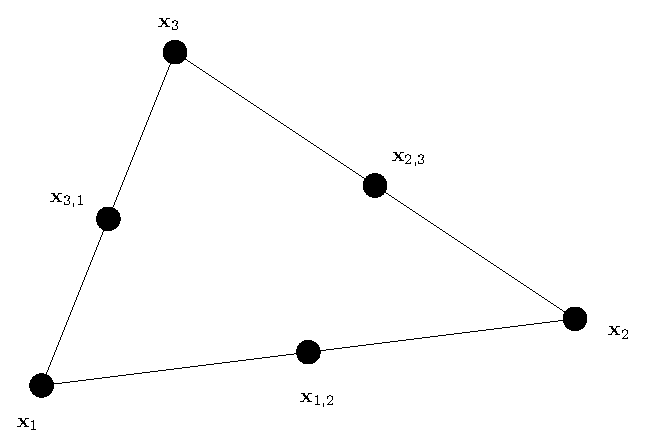
\includegraphics[width=0.6\textwidth]{quadratic-elt}
\par\end{centering}

\caption{\label{fig:Quadratic-Lagrange-element}Quadratic Lagrange element}


\end{figure}


The function that creates the element type data structure for piecewise
quadratic elements is very similar to that for piecewise linear elements.\index{quad2d_elt()@\texttt{quad2d\_elt()}}

\nwenddocs{}\nwbegincode{129}\sublabel{NWpdeB-fil8-I}\nwmargintag{{\nwtagstyle{}\subpageref{NWpdeB-fil8-I}}}\moddef{filelist~{\nwtagstyle{}\subpageref{NWpdeB-fil8-1}}}\plusendmoddef
quad2d-elt.m \\
\nwendcode{}\nwbegincode{130}\sublabel{NWpdeB-quaC-1}\nwmargintag{{\nwtagstyle{}\subpageref{NWpdeB-quaC-1}}}\moddef{quad2d-elt.m~{\nwtagstyle{}\subpageref{NWpdeB-quaC-1}}}\endmoddef
function elt = quad2d_elt() 
% function elt = quad2d_elt() 
% 
% Returns the quadratic 2-D (6-point) element data structure 
nvars = [1;1;1;1;1;1]; 
flist = [1 0 0;
         2 0 0;
         3 0 0;
         1 2 0;
         1 3 0;
         2 3 0]; 
vnodes = [0   0;
          1   0;
          0   1;
          1/2 0;
          0   1/2;
          1/2 1/2];
elt = struct('Aphihat',@quad2d_Aphihat, ...
     'nvars',nvars,'flist',flist, ...
     'pxfeature',@quad2d_pxfeature,'vnodes',vnodes, ...
     'trans_Aphihat',@trans2d_Aphilist); 
end % function

\nwalsodefined{\\{NWpdeB-quaC-2}\\{NWpdeB-quaC-3}}\nwnotused{quad2d-elt.m}\nwendcode{}\nwbegindocs{131}\nwdocspar


\subsubsection{Piecewise quadratic elements: Aphihat()}

This is the main workhorse of the quadratic element data structure:\index{quad2d_Aphihat()@\texttt{quad2d\_Aphihat()}}

\nwenddocs{}\nwbegincode{132}\sublabel{NWpdeB-quaC-2}\nwmargintag{{\nwtagstyle{}\subpageref{NWpdeB-quaC-2}}}\moddef{quad2d-elt.m~{\nwtagstyle{}\subpageref{NWpdeB-quaC-1}}}\plusendmoddef
function Aphilist = quad2d_Aphihat(xhat,order)
% function Aphilist = quad2d_Aphihat(xhat,order)
%
% Returns array of basis functions, their gradient and Hessian entries
% for quadratic basis functions on a 2-D reference triangle at xhat.
% The vertices of the reference triangle are (0,0), (1,0), and (0,1).
% Aphilist(i,j) is the value of the j'th operator on phi_i at xhat.
% Here phi_i is the affine function where phi_i(xhat_j) == 1
% if i == j, and zero otherwise; xhat_i is the i'th vertex listed above.
%
% order is the maximum order of derivatives considered (order <= 2)
%
% Order of operators: Aphi(xhat) = phi(xhat), d/dx1 phi(xhat),
% d/dx2 phi(xhat), d^2/dx1^2 phi(xhat), d^2/dx1.dx2 phi(xhat),
% d^2/dx2^2 phi(xhat).
x = xhat(1);  y = xhat(2);
% basis function values
Aphilist = [2*(1-x-y)*(0.5-x-y);
            2*x*(x-0.5);
            2*y*(y-0.5);
            4*x*(1-x-y);
            4*y*(1-x-y);
            4*x*y];
if order >= 1
    % gradients (rows) of basis functions
    Aphilist1 = [2*(2*(x+y)-1.5), 2*(2*(x+y)-1.5);
                 4*x-1,           0;
                 0,               4*y-1;
                 4*(1-y)-8*x,     -4*x;
                 -4*y,            4*(1-x)-8*y;
                 4*y,             4*x];
    Aphilist = [Aphilist, Aphilist1];
end
if order >= 2
    % Hessian matrix entries of basis functions: dx1^2, dx1.dx2, dx2^2
    Aphilist2 = [4,  4,  4;
                 4,  0,  0;
                 0,  0,  4;
                -8, -4,  0;
                 0, -4, -8;
                 0,  4,  0];
    Aphilist = [Aphilist, Aphilist2];
end % if
end % function 

\nwendcode{}\nwbegindocs{133}\nwdocspar


\subsubsection{Piecewise quadratic elements: pxfeature()}

Again this code is essentially trivial, even though we now have variables
associated with edges rather than only with vertices as in the piecewise
linear case.\index{quad2d_pxfeature()@\texttt{quad2d\_pxfeature()}}

\nwenddocs{}\nwbegincode{134}\sublabel{NWpdeB-quaC-3}\nwmargintag{{\nwtagstyle{}\subpageref{NWpdeB-quaC-3}}}\moddef{quad2d-elt.m~{\nwtagstyle{}\subpageref{NWpdeB-quaC-1}}}\plusendmoddef
function [px_vars,signs] = quad2d_pxfeature(px)
% function [px_vars,signs] = quad2d_pxfeature(px)
%
% Returns the permutation of the variables (px_vars),
% and the sign changes (signs) resulting from a permutation (px)
% applied to a feature of the appropriate dimension (== length(px)).
% This is for the quadratic 2-D triangle elements.
dim = sum(px ~= 0)-1;
switch dim
    case 0 % points
        px_vars = [1]; signs = [1];
    case 1 % edges
        px_vars = [1]; signs = [1];
    otherwise % not a valid feature
        px_vars = []; signs = [];
end % switch
end % function

\nwendcode{}\nwbegindocs{135}\nwdocspar


\subsection{\label{sub:Piecewise-cubic-elements}\index{element!piecewise cubic}Piecewise
cubic elements}

These elements have a nodal basis with nodes at the vertices, at the
1/3 and 2/3 points on each edge, and the centroid of the triangle.
Because they have two node points on each edge, there may need to
be some permutations to ensure correct references to variables (see
\texttt{pxfeature()} below).\index{cub2d_elt()@\texttt{cub2d\_elt()}}

\nwenddocs{}\nwbegincode{136}\sublabel{NWpdeB-fil8-J}\nwmargintag{{\nwtagstyle{}\subpageref{NWpdeB-fil8-J}}}\moddef{filelist~{\nwtagstyle{}\subpageref{NWpdeB-fil8-1}}}\plusendmoddef
cub2d-elt.m \\
\nwendcode{}\nwbegincode{137}\sublabel{NWpdeB-cubB-1}\nwmargintag{{\nwtagstyle{}\subpageref{NWpdeB-cubB-1}}}\moddef{cub2d-elt.m~{\nwtagstyle{}\subpageref{NWpdeB-cubB-1}}}\endmoddef
function elt = cub2d_elt()
% function elt = cub2d_elt()
%
% Returns cubic 2-D (10-point) element data structure
nvars = [1;1;1;2;2;2;1];
flist = [1 0 0;
         2 0 0;
         3 0 0;
         1 2 0;
         1 3 0;
         2 3 0;
         1 2 3];
vnodes = [0   0;
          1   0;
          0   1;
          0   1/3;
          0   2/3;
          1/3 0;
          2/3 0;
          1/3 2/3;
          2/3 1/3;
          1/3 1/3];
elt = struct('Aphihat',@cub2d_Aphihat, ...
    'nvars',nvars,'flist',flist, ...
    'pxfeature',@cub2d_pxfeature,'vnodes',vnodes, ...
    'trans_Aphihat',@trans2d_Aphilist);
end % function

\nwalsodefined{\\{NWpdeB-cubB-2}\\{NWpdeB-cubB-3}}\nwnotused{cub2d-elt.m}\nwendcode{}\nwbegindocs{138}\nwdocspar


\subsubsection{Piecewise cubic elements: Aphihat}

There are six basis functions on the reference element. \index{cub2d_Aphihat()@\texttt{cub2d\_Aphihat()}}

\nwenddocs{}\nwbegincode{139}\sublabel{NWpdeB-cubB-2}\nwmargintag{{\nwtagstyle{}\subpageref{NWpdeB-cubB-2}}}\moddef{cub2d-elt.m~{\nwtagstyle{}\subpageref{NWpdeB-cubB-1}}}\plusendmoddef
function Aphihat = cub2d_Aphihat(xhat,order)
% function Aphihat = cub2d_Aphihat(xhat,order)
%
% Returns basis function values, gradients and Hessian
% entries for Lagrangian cubic basis functions on the
% reference triangle with vertices (0,0), (1,0), and (0,1).
% Each row contains the value, 1st derivatives, and 2nd derivatives 
% of the corresponding basis function on the reference element.
x = xhat(1);
y = xhat(2);
Aphihat0 = [(9/2)*(1-x-y)*(2/3-x-y)*(1/3-x-y);
    (9/2)*x*(x-1/3)*(x-2/3);
    (9/2)*y*(y-1/3)*(y-2/3);
    (27/2)*x*(2/3-x-y)*(1-x-y);
    (27/2)*x*(x-1/3)*(1-x-y);
    (27/2)*y*(2/3-x-y)*(1-x-y);
    (27/2)*y*(y-1/3)*(1-x-y);
    (27/2)*x*y*(x-1/3);
    (27/2)*x*y*(y-1/3);
    27*x*y*(1-x-y)];
if order >= 1
    Aphihat1 = [ ...
      18*x + 18*y - 27*x*y - (27*x^2)/2 - (27*y^2)/2 - 11/2, 18*x + 18*y - 27*x*y - (27*x^2)/2 - (27*y^2)/2 - 11/2;
      (27*x^2)/2 - 9*x + 1, 0;
      0, (27*y^2)/2 - 9*y + 1;
      (81*x^2)/2 + 54*x*y - 45*x + (27*y^2)/2 - (45*y)/2 + 9, (9*x*(6*x + 6*y - 5))/2;
      36*x + (9*y)/2 - 27*x*y - (81*x^2)/2 - 9/2, -(27*x*(x - 1/3))/2;
      (9*y*(6*x + 6*y - 5))/2, (27*x^2)/2 + 54*x*y - (45*x)/2 + (81*y^2)/2 - 45*y + 9;
      -(27*y*(y - 1/3))/2, (9*x)/2 + 36*y - 27*x*y - (81*y^2)/2 - 9/2;
      (9*y*(6*x - 1))/2, (27*x*(x - 1/3))/2;
      (27*y*(y - 1/3))/2, (9*x*(6*y - 1))/2;
      -27*y*(2*x + y - 1), -27*x*(x + 2*y - 1)];
end
if order >= 2
    Aphihat2 = [ ...
      18 - 27*y - 27*x, 18 - 27*y - 27*x, 18 - 27*y - 27*x;
      27*x - 9, 0, 0;
      0, 0, 27*y - 9;
      81*x + 54*y - 45, 54*x + 27*y - 45/2, 27*x;
      36 - 27*y - 81*x, 9/2 - 27*x, 0;
      27*y, 27*x + 54*y - 45/2, 54*x + 81*y - 45;
      0, 9/2 - 27*y, 36 - 81*y - 27*x;
      27*y, 27*x - 9/2, 0;
      0, 27*y - 9/2, 27*x;
      -54*y, 27 - 54*y - 54*x, -54*x];
end
if order == 0
    Aphihat = Aphihat0;
elseif order == 1
    Aphihat = [Aphihat0, Aphihat1];
elseif order == 2
    Aphihat = [Aphihat0, Aphihat1, Aphihat2];
end % if
end % function

\nwendcode{}\nwbegindocs{140}\nwdocspar


\subsubsection{Piecewise cubic elements: pxfeature()}

Here we need to permute the two edge variables.\index{cub2d_pxfeature()@\texttt{cub2d\_pxfeature()}}

\nwenddocs{}\nwbegincode{141}\sublabel{NWpdeB-cubB-3}\nwmargintag{{\nwtagstyle{}\subpageref{NWpdeB-cubB-3}}}\moddef{cub2d-elt.m~{\nwtagstyle{}\subpageref{NWpdeB-cubB-1}}}\plusendmoddef
function [px_vars,signs] = cub2d_pxfeature(px)
% function [px_vars,signs] = cub2d_pxfeature(px)
%
% Returns the permutation of the variables (px_vars),
% and the sign changes (signs) resulting from a permutation (px)
% applied to a feature of the appropriate dimension (== length(px)).
% This is for the quadratic 2-D triangle elements.
dim = sum(px ~= 0)-1;
switch dim
    case 0 % points
        px_vars = [1]; signs = [1];
    case 1 % edges
        px_vars = px; signs = [1 1];
    case 2 % triangles
        px_vars = [1]; signs = [1];
    otherwise % not a valid feature
        px_vars = []; signs = [];
end % switch
end % function

\nwendcode{}\nwbegindocs{142}\nwdocspar


\subsection{\label{sub:Piecewise-constant-elements}Piecewise constant elements}

Piecewise constant functions are either completely constant, or are
discontinuous. This limits their applicability, but they can still
be useful. Their definition for this system follows.\index{const2d_elt()@\texttt{const2d\_elt()}}

\nwenddocs{}\nwbegincode{143}\sublabel{NWpdeB-fil8-K}\nwmargintag{{\nwtagstyle{}\subpageref{NWpdeB-fil8-K}}}\moddef{filelist~{\nwtagstyle{}\subpageref{NWpdeB-fil8-1}}}\plusendmoddef
const2d-elt.m \\
\nwendcode{}\nwbegincode{144}\sublabel{NWpdeB-conD-1}\nwmargintag{{\nwtagstyle{}\subpageref{NWpdeB-conD-1}}}\moddef{const2d-elt.m~{\nwtagstyle{}\subpageref{NWpdeB-conD-1}}}\endmoddef
function elt = const2d_elt()
% function elt = const2d_elt()
%
% Returns constant 2-D triangle element
nvars  = [1];
flist  = [1 2 3];
vnodes = [1/3, 1/3];
elt = struct('Aphihat',@const2d_Aphihat, ...
    'nvars',nvars,'flist',flist, ...
    'pxfeature',@const2d_pxfeature,'vnodes',vnodes, ...
    'trans_Aphihat',@trans2d_Aphilist);
end % function

\nwalsodefined{\\{NWpdeB-conD-2}\\{NWpdeB-conD-3}}\nwnotused{const2d-elt.m}\nwendcode{}\nwbegindocs{145}\nwdocspar

The basis functions are easy to compute:\index{const2d_Aphihat()@\texttt{const2d\_Aphihat()}}

\nwenddocs{}\nwbegincode{146}\sublabel{NWpdeB-conD-2}\nwmargintag{{\nwtagstyle{}\subpageref{NWpdeB-conD-2}}}\moddef{const2d-elt.m~{\nwtagstyle{}\subpageref{NWpdeB-conD-1}}}\plusendmoddef
function Aphilist = const2d_Aphihat(xhat,order)
% function Aphilist = const2d_Aphihat(xhat,order)
%
% Returns array of basis function values, their gradient and Hessian entries
% for constant basis functions on a 2-D reference triangle at xhat.
% Basis function values
Aphilist0 = [1];
if order >= 1
    % Basis gradient values (along rows)
    Aphilist1 = [0 0];
end
if order >= 2
    % Basis hessian values (along rows: d1^2, d1.d2, d2^2)
    Aphilist2 = [0 0 0];
end
if order == 0
    Aphilist = Aphilist0;
elseif order == 1
    Aphilist = [Aphilist0,Aphilist1];
elseif order == 2
    Aphilist = [Aphilist0,Aphilist1,Aphilist2];
end % if
end % function

\nwendcode{}\nwbegindocs{147}\nwdocspar

There is only one variable so changing the orientation does not do
much to the variables.

\nwenddocs{}\nwbegincode{148}\sublabel{NWpdeB-conD-3}\nwmargintag{{\nwtagstyle{}\subpageref{NWpdeB-conD-3}}}\moddef{const2d-elt.m~{\nwtagstyle{}\subpageref{NWpdeB-conD-1}}}\plusendmoddef
function [px_vars,signs] = const2d_pxfeature(px)
% function [px_vars,signs] = const2d_pxfeature(px)
%
% Returns the permutation of the variables (px_vars),
% and the sign changes (signs) resulting from a permutation (px)
% applied to a feature of the appropriate dimension (== length(px)).
% This is for the quadratic 2-D triangle elements.
dim = sum(px ~= 0)-1;
switch dim
    case 2 % triangles
        px_vars = [1]; signs = [1];
    otherwise % not a valid feature
        px_vars = []; signs = [];
end % switch
end % function
\nwendcode{}\nwbegindocs{149}\nwdocspar


\subsection{\label{sub:Vector-elements}Vector elements}

Rather than create a vector element type separately for each scalar
element type, we can create them automatically from the scalar element
type. There is a new transformation routine, and it is here that the
vector character is made apparent. The final result after the transformation
has the columns of the output ordered as $\mathbf{e}_{1}\cdot\phi_{i}(\mathbf{x})$,
$\mathbf{e}_{2}\cdot\phi_{i}(\mathbf{x})$, $\mathbf{e}_{1}\cdot\partial\phi_{i}/\partial x_{1}(\mathbf{x})$,
$\mathbf{e}_{2}\cdot\partial\phi_{i}/\partial x_{1}(\mathbf{x})$,
etc. That is, the components alternate. \index{eltx2_elt()@\texttt{eltx2\_elt()}}

\nwenddocs{}\nwbegincode{150}\sublabel{NWpdeB-fil8-L}\nwmargintag{{\nwtagstyle{}\subpageref{NWpdeB-fil8-L}}}\moddef{filelist~{\nwtagstyle{}\subpageref{NWpdeB-fil8-1}}}\plusendmoddef
eltx2-elt.m \\
\nwendcode{}\nwbegincode{151}\sublabel{NWpdeB-eltB-1}\nwmargintag{{\nwtagstyle{}\subpageref{NWpdeB-eltB-1}}}\moddef{eltx2-elt.m~{\nwtagstyle{}\subpageref{NWpdeB-eltB-1}}}\endmoddef
function eltx2 = eltx2_elt(elt)
% function eltx2 = eltx2_elt(elt)
%
% Returns element data structure with the same basis
% functions as defined by elt, but with 2 components for
% each component of elt.
nvars = elt.nvars;
nvarsx2 = 2*nvars;
flist = elt.flist;
flistx2 = flist;
trans_Aphihat = @(T,Aphilist,order)(transx2(elt.trans_Aphihat,T,Aphilist,order));
pxfeature = @(px)(pxfeaturex2(elt.pxfeature,px));
vnodes = elt.vnodes();
vnodesx2 = zeros(2*size(vnodes,1),size(vnodes,2));
vnodesx2(2*(1:size(vnodes,1))-1,:) = vnodes;
vnodesx2(2*(1:size(vnodes,1)) ,:) = vnodes;
eltx2 = struct('Aphihat',elt.Aphihat, ...
    'nvars',nvarsx2,'flist',flistx2, ...
    'pxfeature',pxfeature,'vnodes',vnodesx2, ...
    'trans_Aphihat',trans_Aphihat);
end % function

\nwalsodefined{\\{NWpdeB-eltB-2}\\{NWpdeB-eltB-3}}\nwnotused{eltx2-elt.m}\nwendcode{}\nwbegindocs{152}\nwdocspar

Note that the original \texttt{Aphihat()} function is used. But we
need new permutation and transformation functions based on the originals.


\subsubsection{Vector elements: pxfeature()}

\nwenddocs{}\nwbegincode{153}\sublabel{NWpdeB-eltB-2}\nwmargintag{{\nwtagstyle{}\subpageref{NWpdeB-eltB-2}}}\moddef{eltx2-elt.m~{\nwtagstyle{}\subpageref{NWpdeB-eltB-1}}}\plusendmoddef
function [px_varsx2,signsx2] = pxfeaturex2(base_pxfeature,px)
% function [px_varsx2,signsx2] = pxfeaturex2(base_pxfeature,px)
%
% Uses base_pxfeature to create pxfeature() function for the "x2" element
[px_vars,signs] = base_pxfeature(px);
px_varsx2 = zeros(1,2*length(px_vars));
signsx2   = zeros(1,2*length(px_vars));
px_varsx2(2*(1:length(px_vars))-1) = 2*px_vars-1;
signsx2(2*(1:length(px_vars))-1)   = signs;
px_varsx2(2*(1:length(px_vars)) )  = 2*px_vars;
signsx2(2*(1:length(px_vars)) )    = signs;
end % function

\nwendcode{}\nwbegindocs{154}\nwdocspar


\subsubsection{Vector elements: trans\_Aphilist()}

\nwenddocs{}\nwbegincode{155}\sublabel{NWpdeB-eltB-3}\nwmargintag{{\nwtagstyle{}\subpageref{NWpdeB-eltB-3}}}\moddef{eltx2-elt.m~{\nwtagstyle{}\subpageref{NWpdeB-eltB-1}}}\plusendmoddef
function Aphilistx2 = transx2(base_trans,T,Aphilist,order)
% function Aphilistx2 = transx2(base_trans,T,Aphilist,order)
%
% Uses base_trans to create trans_Aphilist function for the "x2" element
Aphilist = base_trans(T,Aphilist,order);
nb = size(Aphilist,1);
Aphilistx2 = zeros(2*nb,size(Aphilist,2));
Aphilistx2(2*(1:nb)-1,1) = Aphilist(:,1);
Aphilistx2(2*(1:nb) ,2) = Aphilist(:,1);
if order >= 1
    Aphilistx2(2*(1:nb)-1,3:4) = Aphilist(:,2:3);
    Aphilistx2(2*(1:nb) ,5:6) = Aphilist(:,2:3);
end
if order >= 2
    Aphilistx2(2*(1:nb)-1,7:9) = Aphilist(:,4:6);
    Aphilistx2(2*(1:nb) ,10:12) = Aphilist(:,4:6);
end
end % function

\nwendcode{}\nwbegindocs{156}\nwdocspar


\subsection{$C^{1}$ elements: Bell's triangle}

Work in progress.


\subsection{Stokes' equations: the Arnold--Brezzi--Fortin elements}

Work in progress.

\index{Stokes' equation}Stokes' equations have the form
\begin{eqnarray*}
-\mu\Delta\mathbf{u}+\left(\mathbf{w}\cdot\nabla\right)\mathbf{u} & = & -\nabla p+\mathbf{f}(\mathbf{x}),\\
\nabla\cdot\mathbf{u} & = & 0.
\end{eqnarray*}
This is a natural template for the Navier--Stokes equations for incompressible
Newtonian fluidswhere $\mathbf{u}$ is the velocity field, and $p$
is the pressure field. For $\mathbf{w}=0$, the Stokes equations can
be treated as a constrained optimization problem:
\begin{eqnarray*}
 &  & \min\int_{\Omega}\left[\frac{1}{2}\mu\left|\nabla\mathbf{u}\right|^{2}-\mathbf{f}\cdot\mathbf{u}\right]d\mathbf{x}\qquad\mbox{subject to}\\
 &  & \qquad\nabla\cdot\mathbf{u}=0,
\end{eqnarray*}
where $p$ takes the role of Lagrange multiplier. A global condition
has to be placed on $p$ as otherwise replacing $p$ with $p+c$ for
any constant $c$ gives a new solution. For uniqueness we typically
require that $\int_{\Omega}p\, d\mathbf{x}=0$.

The weak form of Stokes' equations are: for all suitable $\mathbf{v}$
and $q$,
\begin{eqnarray*}
\int_{\Omega}\left[\mu\nabla\mathbf{v}:\nabla\mathbf{u}+\mathbf{v}\cdot\left(\left(\mathbf{w}\cdot\nabla\right)\mathbf{u}\right)-\left(\nabla\cdot\mathbf{v}\right)p\right]d\mathbf{x} & = & \int_{\Omega}\mathbf{v}\cdot\mathbf{f}\, d\mathbf{x}+(\mbox{boundary integrals}),\\
\int_{\Omega}q\left(\nabla\cdot\mathbf{u}\right)\, d\mathbf{x} & = & 0.
\end{eqnarray*}


This can be dealt with in separate ways. We can create separate elements
for $\mathbf{u}$ and $p$, and use \texttt{pgassembly()} to combine
them, or we can create a single element for both together. The \index{element!Arnold--Brezzi--Fortin}Arnold--Brezzi--Fortin
(ABF) finite element method for this problem involves using an enriched
piecewise linear element for each component of $\mathbf{u}$ and piecewise
linear elements for $p$. The additional basis function for each $u_{i}$
has the form $\lambda_{1}\lambda_{2}\lambda_{3}$ in barycentric coordinates,
or in standard coordinates for the reference triangle, $27xy(1-x-y)$.
We can create a scalar ABF element which contains just the four basis
functions necessary, and then use \texttt{eltx2\_elt()} to create
the vector element for $\mathbf{u}$.

The vector element for $\mathbf{u}$ is simply the ABF scalar element
``$\times2$''.\index{abf2d_elt()@\texttt{abf2d\_elt()}}

\nwenddocs{}\nwbegincode{157}\sublabel{NWpdeB-fil8-M}\nwmargintag{{\nwtagstyle{}\subpageref{NWpdeB-fil8-M}}}\moddef{filelist~{\nwtagstyle{}\subpageref{NWpdeB-fil8-1}}}\plusendmoddef
abf2d-elt.m \\
\nwendcode{}\nwbegincode{158}\sublabel{NWpdeB-abfB-1}\nwmargintag{{\nwtagstyle{}\subpageref{NWpdeB-abfB-1}}}\moddef{abf2d-elt.m~{\nwtagstyle{}\subpageref{NWpdeB-abfB-1}}}\endmoddef
function elt = abf2d_elt()
% function elt = abf2d_elt()
%
% ABF vector element for velocity field.
% This is the ABF scalar element "x2".
% The rationale for using this set of basis functions is
% given in Arnold, Brezzi and Fortin, 
%
elt = eltx2_elt(abfs2d_elt());
end % function

\nwalsodefined{\\{NWpdeB-abfB-2}\\{NWpdeB-abfB-3}\\{NWpdeB-abfB-4}\\{NWpdeB-abfB-5}}\nwnotused{abf2d-elt.m}\nwendcode{}\nwbegindocs{159}\nwdocspar

The scalar element is defined below.\index{abfs2d_elt()@\texttt{abfs2d\_elt()}}

\nwenddocs{}\nwbegincode{160}\sublabel{NWpdeB-abfB-2}\nwmargintag{{\nwtagstyle{}\subpageref{NWpdeB-abfB-2}}}\moddef{abf2d-elt.m~{\nwtagstyle{}\subpageref{NWpdeB-abfB-1}}}\plusendmoddef
function elt = abfs2d_elt()
% function elt = abfs2d_elt()
%
% Returns the ABF scalar 2-D (3-point) element data structure.
% The basis functions for this element are the same as for
% the piecewise linear element, plus the "bubble" function
% \\phi_4(x,y) = 27xy(1-x-y). 
nvars = [1;1;1;1]
flist = [1 0 0
         2 0 0
         3 0 0
         1 2 3];
elt = struct('Aphihat',@abfs2d_Aphihat, ...
    'nvars',nvars,'flist',flist, ...
    'pxfeature',@abfs2d_pxfeature,'vnodes',abfs2d_vnodes(), ...
    'trans_Aphihat',@trans2d_Aphilist);
end

\nwendcode{}\nwbegindocs{161}\nwdocspar

Note that the first three basis functions are associated with the
vertices of the triangle; these are linear basis functions. The fourth
is the ``bubble'' function, which is associated with the interior
of the triangle. The basis functions are given below:\index{abfs2d_Aphihat()@\texttt{abfs2d\_Aphihat()}}

\nwenddocs{}\nwbegincode{162}\sublabel{NWpdeB-abfB-3}\nwmargintag{{\nwtagstyle{}\subpageref{NWpdeB-abfB-3}}}\moddef{abf2d-elt.m~{\nwtagstyle{}\subpageref{NWpdeB-abfB-1}}}\plusendmoddef
function Aphilist = abfs2d_Aphihat(xhat,order)
% Aphilist = abfs2d_Aphihat(xhat,order)
%
% ABF scalar element: linear basis functions plus "bubble" function
% \\lambda_1\\lambda_2\\lambda_3 in barycentric coordinates.
x = xhat(1);  y = xhat(2);
% Basis function values
Aphilist0 = [1-x-y; 
             x; 
             y
             27*x*y*(1-x-y)];
if order >= 1
    % Basis gradient values (along rows)
    Aphilist1 = [-1 -1;
                  1  0;
                  0  1;
                 27*y*(1-y-2*x), 27*x*(1-x-2*y)];
end
if order >= 2
    % Basis hessian values (along rows: dx1^2, dx1.dx2, dx2^2)
    Aphilist2 = [0 0 0;
                 0 0 0;
                 0 0 0;
                 -54*y, 27 - 54*y - 54*x, -54*x];
end
if order == 0
    Aphilist = Aphilist0;
elseif order == 1
    Aphilist = [Aphilist0,Aphilist1];
elseif order == 2
    Aphilist = [Aphilist0,Aphilist1,Aphilist2];
end % if
end % function

\nwendcode{}\nwbegindocs{163}\nwdocspar

Permutations of the geometric features do not change the ordering
(or signs) of the variables.\index{abfs2d_pxfeature()@\texttt{abfs2d\_pxfeature()}}

\nwenddocs{}\nwbegincode{164}\sublabel{NWpdeB-abfB-4}\nwmargintag{{\nwtagstyle{}\subpageref{NWpdeB-abfB-4}}}\moddef{abf2d-elt.m~{\nwtagstyle{}\subpageref{NWpdeB-abfB-1}}}\plusendmoddef
function [px_vars,signs] = abfs2d_pxfeature(px)
% function [px_vars,signs] = abfs2d_pxfeature(px)
%
% Returns the permutation of the variables (px_vars),
% and the sign changes (signs) resulting from a permutation (px)
% applied to a feature of the appropriate dimension (== length(px)).
% This is for the linear (or affine) 2-D triangle elements.
dimp1 = sum(px ~= 0);  % dimp1 == dimension plus 1
switch dimp1
    case 1 % points
        px_vars = [1]; signs = [1];
    case 3 % triangles
        px_vars = [1]; signs = [1];
    otherwise % not a valid feature
        px_vars = []; signs = [];
end % switch
end % function

\nwendcode{}\nwbegindocs{165}\nwdocspar

The basis is a nodal basis with nodes at the vertices and the centroid
of the triangle, except that $\phi_{i}$ are not zero at the centroid
for $i=1,\,2,\,3$.

\nwenddocs{}\nwbegincode{166}\sublabel{NWpdeB-abfB-5}\nwmargintag{{\nwtagstyle{}\subpageref{NWpdeB-abfB-5}}}\moddef{abf2d-elt.m~{\nwtagstyle{}\subpageref{NWpdeB-abfB-1}}}\plusendmoddef
function vnodes = abfs2d_vnodes()
% function vnodes = abfs2d_vnodes()
% 
% Returns the positions of the variable nodes
% with respect to the reference element.
% Same format as p (2 x m)
vnodes = [0   0;
          1   0;
          0   1;
          1/3 1/3];
end % function
\nwendcode{}\nwbegindocs{167}\nwdocspar

We need to compute the integrals $\int_{\Omega}q\,\nabla\cdot\mathbf{u}\, d\mathbf{x}$
for $q$ piecewise linear and $\mathbf{u}$ formed using the ABF vector
element, which can be achieved using the following PDE data structure:
\begin{lyxcode}
qdiv\_form~=~struct('coeffs',@(x){[}0,0,1,0,0,1;zeros(2,6){]},~...

~~~~'rhs',@(x)zeros(6,1),~'order',1);
\end{lyxcode}

\subsection{Hsieh--Clough--Tocher $C^{1}$ element}

\index{Hsieh--Clough--Tocher (HCT) element}This is a $C^{1}$ ``macro''
element with piecewise cubic basis functions; these basis functions
are cubic on subtriangles. This element involves normal derivatives
at the midpoints of the edges. Affine transformations do not preserve
normal derivatives, so there is an additional complication in the
computation of the transformation of the basis functions so that the
nodal basis property is preserved in the basis functions on the real
elements.

The element is illustrated in Figure~\ref{fig:Hsieh--Clough--Tocher-elem}.
At each vertex, there are three variables: one for the value at the
point, and two for the two partial derivatives ($\partial\phi/\partial x_{1}$,
$\partial\phi/\partial x_{2}$). Also, at the midpoint of each edge
there is the normal derivative. This gives a total of 12 nodal basis
functions for this element. Integration over these elements should
be done using a composite integration method: the basis functions
are cubic over the sub-triangles formed by an edge and the centroid
($\mathbf{x}_{c}=(\mathbf{x}_{1}+\mathbf{x}_{2}+\mathbf{x}_{3})/3$).

\begin{figure}
\noindent \begin{centering}
\includegraphics[width=0.7\textwidth]{hct-elt}
\par\end{centering}

\caption{\label{fig:Hsieh--Clough--Tocher-elem}Hsieh--Clough--Tocher (HCT)
element}


\end{figure}


\nwenddocs{}\nwbegincode{168}\sublabel{NWpdeB-fil8-N}\nwmargintag{{\nwtagstyle{}\subpageref{NWpdeB-fil8-N}}}\moddef{filelist~{\nwtagstyle{}\subpageref{NWpdeB-fil8-1}}}\plusendmoddef
hct2d-elt.m \\
\nwendcode{}\nwbegincode{169}\sublabel{NWpdeB-hctB-1}\nwmargintag{{\nwtagstyle{}\subpageref{NWpdeB-hctB-1}}}\moddef{hct2d-elt.m~{\nwtagstyle{}\subpageref{NWpdeB-hctB-1}}}\endmoddef
function elt = hct2d_elt()
% function elt = hct2d_elt()
%
% Hsieh-Clough-Tocher element in two dimensions.
nvars = [3;3;3;1;1;1];
flist = [1 0 0;  1 0 0;  1 0 0;
         2 0 0;  2 0 0;  2 0 0;
         3 0 0;  3 0 0;  3 0 0;
         1 2 0;
         1 3 0;
         2 3 0];
vnodes = [0 0;  0 0;  0 0;
          1 0;  1 0;  1 0;
          0 1;  0 1;  0 1;
          1/2 0; 0 1/2; 1/2 1/2];
elt = struct('Aphihat',@hct2d_Aphihat, ...
    'nvars',nvars,'flist',flist, ...
    'pxfeature',@hct2d_pxfeature,'vnodes',vnodes, ...
    'trans_Aphihat',@hct2d_trans_Aphilist);
end
end % function
 
\nwalsodefined{\\{NWpdeB-hctB-2}}\nwnotused{hct2d-elt.m}\nwendcode{}\nwbegindocs{170}\nwdocspar

There are twelve basis functions for one HCT element, but the formula
used depends on which part of the reference triangle needs to be evaluated.

\nwenddocs{}\nwbegincode{171}\sublabel{NWpdeB-hctB-2}\nwmargintag{{\nwtagstyle{}\subpageref{NWpdeB-hctB-2}}}\moddef{hct2d-elt.m~{\nwtagstyle{}\subpageref{NWpdeB-hctB-1}}}\plusendmoddef
\nwendcode{}\nwbegindocs{172}\nwdocspar


\subsection{Three-dimensional elements}


\subsubsection{\index{element!piecewise linear (3D)}Piecewise linear three-dimensional
elements}

This is the simplest useful three-dimensional element. Assembly routines
for three-dimensional problems need to be written. (See Section~\ref{sec:Matrix-assembly-code}.)
See Section~\ref{sub:Piecewise-linear-elements} for the two-dimensional
piecewise linear element. 

Note that the order of the operators for scalar three-dimensional
elements is $\mathcal{A}=I$ (identity), $\partial/\partial x_{1}$,
$\partial/\partial x_{2}$, $\partial/\partial x_{3}$, $\partial^{2}/\partial x_{1}^{2}$,
$\partial^{2}/\partial x_{1}\partial x_{2}$, $\partial^{2}/\partial x_{1}\partial x_{3}$,
$\partial^{2}/\partial x_{2}^{2}$, $\partial^{2}/\partial x_{2}\partial x_{3}$,
$\partial^{2}/\partial x_{3}^{2}$. We often use the notation $x=x_{1}$,
$y=x_{2}$ and $z=x_{3}$ for convenience.

Note that all basis functions are associated with vertices of the
tetrahedron. We also need a new transformation routines for transforming
from the reference element in three dimensions (which is the tetrahedron
with the vertices $(0,0,0)$, $(1,0,0)$, $(0,1,0)$, and $(0,0,1)$)
to the actual element (with vertices $\mathbf{p}_{1}$, $\mathbf{p}_{2}$,
$\mathbf{p}_{3}$ and $\mathbf{p}_{4}$).\index{lin3d_elt()@\texttt{lin3d\_elt()}}

\nwenddocs{}\nwbegincode{173}\sublabel{NWpdeB-fil8-O}\nwmargintag{{\nwtagstyle{}\subpageref{NWpdeB-fil8-O}}}\moddef{filelist~{\nwtagstyle{}\subpageref{NWpdeB-fil8-1}}}\plusendmoddef
lin3d-elt.m \\
\nwendcode{}\nwbegincode{174}\sublabel{NWpdeB-linB.2-1}\nwmargintag{{\nwtagstyle{}\subpageref{NWpdeB-linB.2-1}}}\moddef{lin3d-elt.m~{\nwtagstyle{}\subpageref{NWpdeB-linB.2-1}}}\endmoddef
function elt = lin3d_elt()
% function elt = lin3d_elt()
%
% Returns the linear 3-D (4-point) element data structure.
nvars = [1;1;1;1];
flist = [1 0 0 0;
         2 0 0 0;
         3 0 0 0;
         4 0 0 0];
vnodes = [0 0 0;
          1 0 0;
          0 1 0;
          0 0 1];
elt = struct('Aphihat',@lin3d_Aphihat, ...
    'nvars',nvars,'flist',flist, ...
    'pxfeature',@lin3d_pxfeature,'vnodes',vnodes, ...
    'trans_Aphihat',@trans3d_Aphilist);
end

\nwalsodefined{\\{NWpdeB-linB.2-2}\\{NWpdeB-linB.2-3}}\nwnotused{lin3d-elt.m}\nwendcode{}\nwbegindocs{175}\nwdocspar

The basis functions are easily computed. Note that the first derivatives
are constant, and the second derivatives are all zero.\index{lin3d_Aphihat()@\texttt{lin3d\_Aphihat()}}

\nwenddocs{}\nwbegincode{176}\sublabel{NWpdeB-linB.2-2}\nwmargintag{{\nwtagstyle{}\subpageref{NWpdeB-linB.2-2}}}\moddef{lin3d-elt.m~{\nwtagstyle{}\subpageref{NWpdeB-linB.2-1}}}\plusendmoddef
function Aphilist = lin3d_Aphihat(xhat,order)
% Aphilist = lin3d_Aphihat(xhat,order)
%
% Returns array of basis function values, their gradient and Hessian entries
x = xhat(1);  y = xhat(2);  z = xhat(3);
% Basis function values
Aphilist0 = [1-x-y-z; 
             x; 
             y;
             z];
if order >= 1
    % Basis gradient values (along rows)
    Aphilist1 = [-1 -1 -1;
                  1  0  0;
                  0  1  0;
                  0  0  1];
end
if order >= 2
    % Basis Hessian values (along rows: dx1^2, dx1.dx2, dx1.dx3, dx2^2, dx2.dx3, dx3^2)
    Aphilist2 = [0 0 0 0 0 0;
                 0 0 0 0 0 0;
                 0 0 0 0 0 0];
end
if order == 0
    Aphilist = Aphilist0;
elseif order == 1
    Aphilist = [Aphilist0,Aphilist1];
elseif order == 2
    Aphilist = [Aphilist0,Aphilist1,Aphilist2];
end % if
end % function

\nwendcode{}\nwbegindocs{177}\nwdocspar

Permutation of the geometric features does not change the order of
the variables since there is only one variable for each vertex, just
as for the two-dimensional piecewise linear element.\index{lin3d_pxfeature()@\texttt{lin3d\_pxfeature()}}

\nwenddocs{}\nwbegincode{178}\sublabel{NWpdeB-linB.2-3}\nwmargintag{{\nwtagstyle{}\subpageref{NWpdeB-linB.2-3}}}\moddef{lin3d-elt.m~{\nwtagstyle{}\subpageref{NWpdeB-linB.2-1}}}\plusendmoddef
function [px_vars,signs] = lin3d_pxfeature(px)
% function [px_vars,signs] = lin3d_pxfeature(px)
%
% Returns the permutation of the variables (px_vars),
% and the sign changes (signs) resulting from a permutation (px)
% applied to a feature of the appropriate dimension (== length(px)).
% This is for the linear (or affine) 3-D tetrahedral elements.
dimp1 = sum(px ~= 0);  % dimp1 == dimension plus 1
switch dimp1
    case 1 % points
        px_vars = [1]; signs = [1];
    otherwise % not a valid feature
        px_vars = []; signs = [];
end % switch
end % function

\nwendcode{}\nwbegindocs{179}\nwdocspar


\subsection{Three-dimensional scalar transformations}

The affine transformation in three dimensions $\widehat{\mathbf{x}}\mapsto\mathbf{x}=T\widehat{\mathbf{x}}+\mathbf{b}$
must modify the derivative values. For derivation of the basic equations,
see Section~\ref{sub:Transformation-scalar-Lagrange-elements}.\index{trans3d_Aphilist()@\texttt{trans3d\_Aphilist()}}

\nwenddocs{}\nwbegincode{180}\sublabel{NWpdeB-fil8-P}\nwmargintag{{\nwtagstyle{}\subpageref{NWpdeB-fil8-P}}}\moddef{filelist~{\nwtagstyle{}\subpageref{NWpdeB-fil8-1}}}\plusendmoddef
trans3d-Aphilist.m \\
\nwendcode{}\nwbegincode{181}\sublabel{NWpdeB-traI.2-1}\nwmargintag{{\nwtagstyle{}\subpageref{NWpdeB-traI.2-1}}}\moddef{trans3d-Aphilist.m~{\nwtagstyle{}\subpageref{NWpdeB-traI.2-1}}}\endmoddef
function Aphilist2 = trans3d_Aphilist(T,Aphilist,order)
% function Aphilist2 = trans3d_Aphilist(T,Aphilist,order)
%
% Transforms Aphilist into Aphilist2 according to matrix T (3 x 3)
% Note: Order of colums is [val, d/dx1, d/dx2, d/dx3, d^2/dx1^2, d^2/dx1.dx2, d^2/dx1.dx3, d^2/dx2^2, d^2/dx2.dx3, d^2/dx3^2]
Aphilist2 = zeros(size(Aphilist));
Aphilist2(:,1) = Aphilist(:,1); % values unchanged
if order >= 1
    S = inv(T);
    Aphilist2(:,2:4) = Aphilist(:,2:4)*S; % chain rule for 1st derivatives
end % if
if order >= 2
    % chain rule for 2nd derivatives (affine transformation)
    Aphilist2(:,5)  = Aphilist(:,5)*(S(1,1)^2)+ ...
           Aphilist(:,6)*(2*S(2,1)*S(1,1))+ ...
           Aphilist(:,7)*(2*S(3,1)*S(1,1))+ ...
           Aphilist(:,8)*(S(2,1)^2)+ ...
           Aphilist(:,9)*(2*S(3,1)*S(2,1))+ ...
           Aphilist(:,10)*(S(3,1)^2);
    Aphilist2(:,6)  = Aphilist(:,5)*(S(1,1)*S(1,2))+ ...
           Aphilist(:,6)*(S(1,1)*S(2,2)+S(1,2)*S(2,1))+ ...
           Aphilist(:,7)*(S(3,1)*S(1,2)+S(1,1)*S(3,2))+ ...
           Aphilist(:,8)*(S(2,2)*S(2,1))+ ...
           Aphilist(:,9)*(S(3,1)*S(2,2)+S(2,1)*S(3,2))+ ...
           Aphilist(:,10)*(S(3,1)*S(3,2));
    Aphilist2(:,7)  = Aphilist(:,5)*(S(1,1)*S(1,3))+ ...
           Aphilist(:,6)*(S(2,1)*S(1,3)+S(1,1)*S(2,3))+ ...
           Aphilist(:,7)*(S(3,1)*S(1,3)+S(1,1)*S(3,3))+ ...
           Aphilist(:,8)*(S(2,1)*S(2,3))+ ...
           Aphilist(:,9)*(S(3,1)*S(2,3)+S(2,1)*S(3,3))+ ...
           Aphilist(:,10)*(S(3,1)*S(3,3));
    Aphilist2(:,8)  = Aphilist(:,5)*(S(1,2)^2)+ ...
           Aphilist(:,6)*(2*S(2,2)*S(1,2))+ ...
           Aphilist(:,7)*(2*S(3,2)*S(1,2))+ ...
           Aphilist(:,8)*(S(2,2)^2)+ ...
           Aphilist(:,9)*(2*S(3,2)*S(2,2))+ ...
           Aphilist(:,10)*(S(3,2)^2);
    Aphilist2(:,9)  = Aphilist(:,5)*(S(1,2)*S(1,3))+ ...
           Aphilist(:,6)*(S(2,2)*S(1,3)+S(1,2)*S(2,3))+ ...
           Aphilist(:,7)*(S(3,2)*S(1,3)+S(1,2)*S(3,3))+ ...
           Aphilist(:,8)*(S(2,2)*S(2,3))+ ...
           Aphilist(:,9)*(S(3,2)*S(2,3)+S(2,2)*S(3,3))+ ...
           Aphilist(:,10)*(S(3,2)*S(3,3));
    Aphilist2(:,10) = Aphilist(:,5)*(S(1,3)^2)+ ...
           Aphilist(:,6)*(2*S(2,3)*S(1,3))+ ...
           Aphilist(:,7)*(2*S(3,3)*S(1,3))+ ...
           Aphilist(:,8)*(S(2,3)^2)+ ...
           Aphilist(:,9)*(2*S(3,3)*S(2,3))+ ...
           Aphilist(:,10)*(S(3,3)^2);
end % if
end % function

\nwnotused{trans3d-Aphilist.m}\nwendcode{}\nwbegindocs{182}\nwdocspar


\section{\label{sec:Numerical-integration}Numerical integration\index{integration}}

Numerical integration is basic to the assembly process. The numerical
integration routine should be exact for products of the basis functions
that are used. Since the assembly routines perform the transformation
from reference elements, these routines just need to return the points
and weights for the method on a reference element, which is the triangle
with vertices $(0,0)$, $(1,0)$, and $(0,1)$. 


\subsection{\label{sub:Two-dimensional-integration}Two-dimensional integration
methods}


\subsubsection{\label{sub:Centroid-method}Centroid method\index{integration!centroid method}}

This is a one-point method with order 1. (That is, it is exact for
all polynomials of order $\leq1$.)\index{int2d_centroid1()@\texttt{int2d\_centroid1()}}

\nwenddocs{}\nwbegincode{183}\sublabel{NWpdeB-fil8-Q}\nwmargintag{{\nwtagstyle{}\subpageref{NWpdeB-fil8-Q}}}\moddef{filelist~{\nwtagstyle{}\subpageref{NWpdeB-fil8-1}}}\plusendmoddef
int2d-centroid1.m \\
\nwendcode{}\nwbegincode{184}\sublabel{NWpdeB-intH-1}\nwmargintag{{\nwtagstyle{}\subpageref{NWpdeB-intH-1}}}\moddef{int2d-centroid1.m~{\nwtagstyle{}\subpageref{NWpdeB-intH-1}}}\endmoddef
function [p,w] = int2d_centroid1()
% function [p,w] = int2d_centroid1()
%
% This is the simplest triangle integration method.
p = [1/3, 1/3];
w = 1/2;
\nwnotused{int2d-centroid1.m}\nwendcode{}\nwbegindocs{185}\nwdocspar


\subsubsection{\label{sub:Radon-method}Radon's method\index{integration!Radon's method}}

This is a 7-point method with order 5 \cite{rad:zmk}.\index{int2d_radon7()@\texttt{int2d\_radon7()}}

\nwenddocs{}\nwbegincode{186}\sublabel{NWpdeB-fil8-R}\nwmargintag{{\nwtagstyle{}\subpageref{NWpdeB-fil8-R}}}\moddef{filelist~{\nwtagstyle{}\subpageref{NWpdeB-fil8-1}}}\plusendmoddef
int2d-radon7.m \\
\nwendcode{}\nwbegincode{187}\sublabel{NWpdeB-intE-1}\nwmargintag{{\nwtagstyle{}\subpageref{NWpdeB-intE-1}}}\moddef{int2d-radon7.m~{\nwtagstyle{}\subpageref{NWpdeB-intE-1}}}\endmoddef
function [p,w] = int2d_radon7()
% function [p,w] = int2d_radon7()
%
% Returns the points (p) and weights (w) of J. Radon's 7-point
% integration formula for the triangle with vertices (0,0), (1,0), (0,1).
% This formula is exact for polynomials up to degree 5.
% Points are the rows of p.
%
% Reference: J. Radon, Zur mechanischen Kubatur. (German)
% Monatsh. Math. 52, (1948), pp. 286-300.
p = [1/3,              1/3;
    (6+sqrt(15))/21,   (9-2*sqrt(15))/21;
    (9-2*sqrt(15))/21, (6+sqrt(15))/21;
    (6+sqrt(15))/21,   (6+sqrt(15))/21;
    (6-sqrt(15))/21,   (9+2*sqrt(15))/21;
    (9+2*sqrt(15))/21, (6-sqrt(15))/21;
    (6-sqrt(15))/21,   (6-sqrt(15))/21];
w = [9/80;
    (155+sqrt(15))/2400;
    (155+sqrt(15))/2400;
    (155+sqrt(15))/2400;
    (155-sqrt(15))/2400;
    (155-sqrt(15))/2400;
    (155-sqrt(15))/2400];
end
\nwnotused{int2d-radon7.m}\nwendcode{}\nwbegindocs{188}\nwdocspar


\subsubsection{\label{sub:Gatermann-method}Gatermann's method\index{integration!Gatermann's method}}

This is a 12-point method with order 7 \cite{gat:cscfst}.\index{int2d_gatermann12()@\texttt{int2d\_gatermann12()}}

\nwenddocs{}\nwbegincode{189}\sublabel{NWpdeB-fil8-S}\nwmargintag{{\nwtagstyle{}\subpageref{NWpdeB-fil8-S}}}\moddef{filelist~{\nwtagstyle{}\subpageref{NWpdeB-fil8-1}}}\plusendmoddef
int2d-gatermann12.m \\
\nwendcode{}\nwbegincode{190}\sublabel{NWpdeB-intJ-1}\nwmargintag{{\nwtagstyle{}\subpageref{NWpdeB-intJ-1}}}\moddef{int2d-gatermann12.m~{\nwtagstyle{}\subpageref{NWpdeB-intJ-1}}}\endmoddef
function [p,w] = int2d_gatermann12()
% function [p,w] = int2d_gatermann12()
%
% Returns the points (p) and weights (w) of K. Gatermann's 12-point
% integration formula for the triangle with vertices (0,0), (1,0), (0,1).
% This formula is exact for polynomials up to degree 7.
% Points are the rows of p.
%
% Reference: The Construction of Symmetric Cubature Formulas
% for the Square and the Triangle, Computing 40, 229 - 240 (1988)
p = [0.06751786707392436, 0.8700998678316848;  % 1
     0.06238226509439084, 0.06751786707392436; % 2
     0.8700998678316848,  0.06238226509439084; % 3
     0.3215024938520156,  0.6232720494910644;  % 4
     0.05522545665692000, 0.3215024938520156;  % 5
     0.6232720494910644,  0.05522545665692000; % 6
     0.6609491961867980,  0.3047265008681072;  % 7
     0.03432430294509488, 0.6609491961867980;  % 8
     0.3047265008681072,  0.03432430294509488; % 9
     0.2777161669764050,  0.2064414986699949;  % 10
     0.5158423343536001,  0.2777161669764050;  % 11
     0.2064414986699949,  0.5158423343536001]; % 12
w = [0.02651702815743450;
     0.02651702815743450;
     0.02651702815743450;
     0.04388140871444811;
     0.04388140871444811;
     0.04388140871444811;
     0.02877504278497528;
     0.02877504278497528;
     0.02877504278497528;
     0.06749318700980879;
     0.06749318700980879;
     0.06749318700980879];
end
\nwnotused{int2d-gatermann12.m}\nwendcode{}\nwbegindocs{191}\nwdocspar


\subsubsection{\label{sub:integration-Dunavant}A method of Dunavant\index{integration!Dunavant method}}

This is a 33-point method with order 12 \cite{dun:hdesgqrt}.\index{int2d_dunavant33()@\texttt{int2d\_dunavant33()}}

\nwenddocs{}\nwbegincode{192}\sublabel{NWpdeB-fil8-T}\nwmargintag{{\nwtagstyle{}\subpageref{NWpdeB-fil8-T}}}\moddef{filelist~{\nwtagstyle{}\subpageref{NWpdeB-fil8-1}}}\plusendmoddef
int2d-dunavant33.m \\
\nwendcode{}\nwbegincode{193}\sublabel{NWpdeB-intI-1}\nwmargintag{{\nwtagstyle{}\subpageref{NWpdeB-intI-1}}}\moddef{int2d-dunavant33.m~{\nwtagstyle{}\subpageref{NWpdeB-intI-1}}}\endmoddef
function [p,w] = int2d_dunavant33()
% function [p,w] = int2d_dunavant33()
%
% Returns points and weights for Dunavant (1978)'s 
% 12th order 33 point triangle integration method.
% Values taken directly from Dunavant's paper:
% "High degree efficient symmetrical Gaussian quadrature rules for the
% triangle", Internat. J. Numer. Methods Eng. vol 21, pp. 1129-1148 (1985)
% p=12 ng=33 nsige17.8 ssqa9.d-58 error= 1.d-27 ifn= 2439 infers1 time= 74
% weight alpha beta gamma
% 0.025731066440455 0.023565220452390 0.488217389773805 0.488217389773805
% 0.043692544538038 0.120551215411079 0.439724392294460 0.439724392294460
% 0.062858224217885 0.457579229975768 0.271210385012116 0.271210385012116
% 0.034796112930709 0.744847708916828 0.127576145541586 0.127576145541586
% 0.006166261051559 0.957365299093579 0.021317350453210 0.021317350453210
% 0.040371557766381 0.115343494534698 0.275713269685514 0.608943235779788
% 0.022356773202303 0.022838332222257 0.281325580989940 0.695836086787803
% 0.017316231108659 0.025734050548330 0.116251915907597 0.858014033544073
table = [...
0.025731066440455 0.023565220452390 0.488217389773805 0.488217389773805
0.043692544538038 0.120551215411079 0.439724392294460 0.439724392294460
0.062858224217885 0.457579229975768 0.271210385012116 0.271210385012116
0.034796112930709 0.744847708916828 0.127576145541586 0.127576145541586
0.006166261051559 0.957365299093579 0.021317350453210 0.021317350453210
0.040371557766381 0.115343494534698 0.275713269685514 0.608943235779788
0.022356773202303 0.022838332222257 0.281325580989940 0.695836086787803
0.017316231108659 0.025734050548330 0.116251915907597 0.858014033544073];
idx = 1; t_idx = 1;
p = zeros(33,2); w = zeros(32,1);
for t_idx = 1:size(table,1)
    if table(t_idx,3) == table(t_idx,4)
        % 3 entries
        w(idx:(idx+2)) = table(t_idx,1);
        p(idx+0,:) = table(t_idx,[2,3]);
        p(idx+1,:) = table(t_idx,[3,2]);
        p(idx+2,:) = table(t_idx,[3,4]);
        idx = idx+3;
    else
        % 6 entries
        w(idx:(idx+5)) = table(t_idx,1);
        p(idx+0,:) = table(t_idx,[2,3]);
        p(idx+1,:) = table(t_idx,[2,4]);
        p(idx+2,:) = table(t_idx,[3,2]);
        p(idx+3,:) = table(t_idx,[3,4]);
        p(idx+4,:) = table(t_idx,[4,2]);
        p(idx+5,:) = table(t_idx,[4,3]);
        idx = idx+6;
    end % if
end % for
w = w/2;
end % function
\nwnotused{int2d-dunavant33.m}\nwendcode{}\nwbegindocs{194}\nwdocspar


\subsection{\label{sub:One-dimensional-integration}One-dimensional integration
methods}


\subsubsection{\label{sub:Gauss--Legendre-quadrature}Gauss--Legendre quadrature\index{integration!Gauss--Legendre quadrature}}

Here we use the 5-point Gauss--Legendre quadrature method which is
a 9th order method \cite{atk:ina}.\index{int1d_gauss5()@\texttt{int1d\_gauss5()}}

\nwenddocs{}\nwbegincode{195}\sublabel{NWpdeB-fil8-U}\nwmargintag{{\nwtagstyle{}\subpageref{NWpdeB-fil8-U}}}\moddef{filelist~{\nwtagstyle{}\subpageref{NWpdeB-fil8-1}}}\plusendmoddef
int1d-gauss5.m \\
\nwendcode{}\nwbegincode{196}\sublabel{NWpdeB-intE.2-1}\nwmargintag{{\nwtagstyle{}\subpageref{NWpdeB-intE.2-1}}}\moddef{int1d-gauss5.m~{\nwtagstyle{}\subpageref{NWpdeB-intE.2-1}}}\endmoddef
function [p,w] = int1d_gauss5()
% function [p,w] = int1d_gauss5()
%
% Returns points and weights for a 5-point Gauss rule
% in 1-D for the interval [0,1]
p = [1/2; (1+sqrt(5-2*sqrt(10/7))/3)/2; (1-sqrt(5-2*sqrt(10/7))/3)/2; ...
     (1+sqrt(5+2*sqrt(10/7))/3)/2; (1-sqrt(5+2*sqrt(10/7))/3)/2];
w = 0.5*[128/225; (322+13*sqrt(70))/900; (322+13*sqrt(70))/900; ...
     (322-13*sqrt(70))/900; (322-13*sqrt(70))/900];
\nwnotused{int1d-gauss5.m}\nwendcode{}\nwbegindocs{197}\nwdocspar


\subsection{\label{sub:Three-dimensional-integration}Three-dimensional integration\index{integration!three-dimensional}}


\subsubsection{\index{integration!centroid method}Centroid method}

This integration method is exact for 1st order polynomials (affine
functions), and uses one point.\index{int3d_centroid1()@\texttt{int3d\_centroid1()}}

\nwenddocs{}\nwbegincode{198}\sublabel{NWpdeB-fil8-V}\nwmargintag{{\nwtagstyle{}\subpageref{NWpdeB-fil8-V}}}\moddef{filelist~{\nwtagstyle{}\subpageref{NWpdeB-fil8-1}}}\plusendmoddef
int3d-centroid1.m \\
\nwendcode{}\nwbegincode{199}\sublabel{NWpdeB-intH.2-1}\nwmargintag{{\nwtagstyle{}\subpageref{NWpdeB-intH.2-1}}}\moddef{int3d-centroid1.m~{\nwtagstyle{}\subpageref{NWpdeB-intH.2-1}}}\endmoddef
function [p,w] = int3d_centroid1()
% function [p,w] = int3d_centroid1()
%
% This is the simplest triangle integration method.
p = [1/4, 1/4, 1/4];
w = 1/6;
\nwnotused{int3d-centroid1.m}\nwendcode{}\nwbegindocs{200}\nwdocspar


\subsection{\label{sub:Composite-integration-rules}\index{integration!composite}Composite
integration rules}

Composite integration rules allow the same integration rule to be
replicated across a collection of sub-triangles. These are particularly
useful for ``macro'' elements, that are formed by piecewise polynomial
functions on sub-triangles of the reference triangle, such as the
HCT element\index{Hsieh--Clough--Tocher (HCT) element}. In the same
way, we can create composite rules that replicate a pre-existing two-dimensional
rule (\texttt{intmethod}) across a triangulation (\texttt{pr},\texttt{tr})
of the reference element.

\nwenddocs{}\nwbegincode{201}\sublabel{NWpdeB-fil8-W}\nwmargintag{{\nwtagstyle{}\subpageref{NWpdeB-fil8-W}}}\moddef{filelist~{\nwtagstyle{}\subpageref{NWpdeB-fil8-1}}}\plusendmoddef
int2d-comp.m \\
\nwendcode{}\nwbegincode{202}\sublabel{NWpdeB-intC-1}\nwmargintag{{\nwtagstyle{}\subpageref{NWpdeB-intC-1}}}\moddef{int2d-comp.m~{\nwtagstyle{}\subpageref{NWpdeB-intC-1}}}\endmoddef
function compmethod = int2d_comp(pr,tr,intmethod)
% function compmethod = int2d_comp(pr,tr,intmethod)
% 
% Returns function handle for composite integration
% method that uses intmethod() as the basic method.
% replicated across all triangles of the triangulation
% (pr,tr) of the reference element.
compmethod = @int2d_comp_func(pr,tr,intmethod);
end function

function [p_int,w_int] = int2d_comp_function(pr,tr,intmethod)
% function [p_int,w_int] = int2d_comp_function(pr,tr,intmethod)
%
% Internal function for int2d_comp().
% This is where the work gets done.
[p_base,w_base] = intmethod(); % base method points & weights
base_len = size(p_base,1);
p_int = zeros(size(tr,1)*base_len,2);
w_int = zeros(size(tr,1)*base_len,1);
for j = 1:size(tr,1)
    % For sub-triangle j...
    % Create affine transformation
    i1 = tr(i,1);  i2 = tr(i,2);  i3 = tr(i,3);
    T = [pr(i2,:)'-pr(i1,:)', pr(i3,:)'-pr(i1,:)'];
    b0 = pr(i1,:)';
    % transform weights and points and add to list
    detT = abs(det(T));
    p_int(((j-1)*base_len+1):(j*base_len),:) = p_base*T'+b0';
    w_int(((j-1)*base_len+1):(j*base_len))   = w_int*detT;
end % for
end % function
\nwnotused{int2d-comp.m}\nwendcode{}\nwbegindocs{203}\nwdocspar

For the HCT element\index{Hsieh--Clough--Tocher (HCT) element}, the
appropriate integration method can be created using something like:

\nwenddocs{}\nwbegincode{204}\sublabel{NWpdeB-HCTE-1}\nwmargintag{{\nwtagstyle{}\subpageref{NWpdeB-HCTE-1}}}\moddef{HCT integrator~{\nwtagstyle{}\subpageref{NWpdeB-HCTE-1}}}\endmoddef
pr = [0,0; 1,0; 0,1; 1/3,1/3];
tr = [1 2 4; 1 3 4; 2 3 4];
int2d_hct = int2d_comp(pr,tr,@int2d_radon7);
\nwnotused{HCT\ integrator}\nwendcode{}\nwbegindocs{205}\nwdocspar


\section{Adaptation}

Adaptation of the mesh is a very useful technique to improve accuracy
at minimal cost. There are two parts to this: one is to use \emph{a
posteriori} error estimation to identify triangles that should be
refined; the other is to solve the refined system of equations. Simple
adaptation techniques result in non-conforming triangulations. This
is illustrated in Figure~\ref{fig:mesh-adaptation}, which shows
hanging nodes from the refined triangles that do not match nodes in
the unrefined triangles on the upper-left.

The fact that we have a non-conforming mesh means that we cannot use
the output of assembly routines ``as is''. The variables associated
with the non-conforming part of the mesh need to be represented in
terms of variables in the unrefined triangles.

\begin{figure}
\noindent \begin{centering}
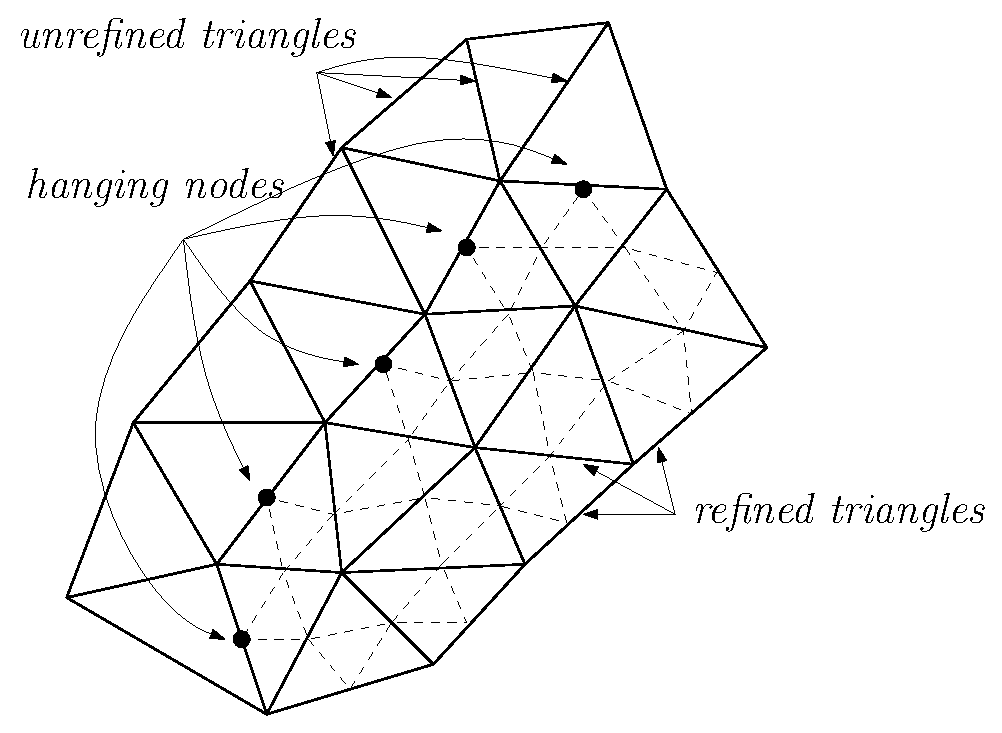
\includegraphics[width=0.9\textwidth]{adaptation-mesh}
\par\end{centering}

\caption{\label{fig:mesh-adaptation}Adaptation of mesh showing hanging nodes}


\end{figure}


The approach we take to mesh refinement starts with the refinement
for the reference element; we take this to be the \emph{reference
refinement}. This reference refinement is a triangulation of the reference
element. The basic assumption is that the basis functions on the reference
element $\widehat{\phi}_{i}$ can be represented as linear combinations
of the basis functions of the reference refinement. This is clearly
the case for piecewise polynomial Lagrange elements, since on each
triangle all polynomials up to a specified degree can be represented.
This is not so for Bell's triangle, since in that element, the basis
functions are 5th order polynomials where the normal derivatives on
the boundaries are cubic. Thus for a non-trivial refinement of the
reference element, the edges of the triangles in the interior of the
reference element will not typically have cubic normal derivatives. 

The basic idea in this code is to represent variables in the refined
triangles in terms of the variables in the unrefined triangles where
they meet. Thus we only need to consider the variables associated
with the edges common to both refined and unrefined triangle. We assume
that every basis function on the reference element is a linear combination
of basis functions for the reference refinement:
\[
\widehat{\phi}_{i}=\sum_{j}b_{ij}\,\widetilde{\phi}_{j},
\]
where $\widetilde{\phi}_{j}$ are the basis functions on the reference
refinement.

Assuming that the corresponding basis function on the real element
is $\phi_{k}(\mathbf{x})=\widehat{\phi}_{i}(\widehat{\mathbf{x}})$
where $\mathbf{x}=T_{K}\widehat{\mathbf{x}}+\mathbf{b}_{K}$, this
relation between $\widehat{\phi}_{i}$ and $\widetilde{\phi}_{j}$
can be transformed from the reference element to the real unrefined
and real refined elements. 

The refined and unrefined triangles are then treated as logically
separated (and the assembly is performed on them that way) until they
are ``glued'' together using sparse matrix-matrix multiplication
with the $b_{ij}$ matrices. Note that the computational cost of this
extra work depends on the number of basis functions associated with
the common boundary between the refined and unrefined triangles. It
is desirable to keep this from growing too large, especially after
many steps of adaptation. The following approach is taken to prevent
excessively large boundaries: the original triangulation is kept,
and each triangle, even if refined many times, has a link to its ``parent''
triangle at the next coarser level. A group of refined triangles can
be unrefined whenever desired. Thus there can be a hierarchy of levels
of refinement. This is illustrated in Figure~\ref{fig:Refinement-levels}.

\begin{figure}
\noindent \begin{centering}
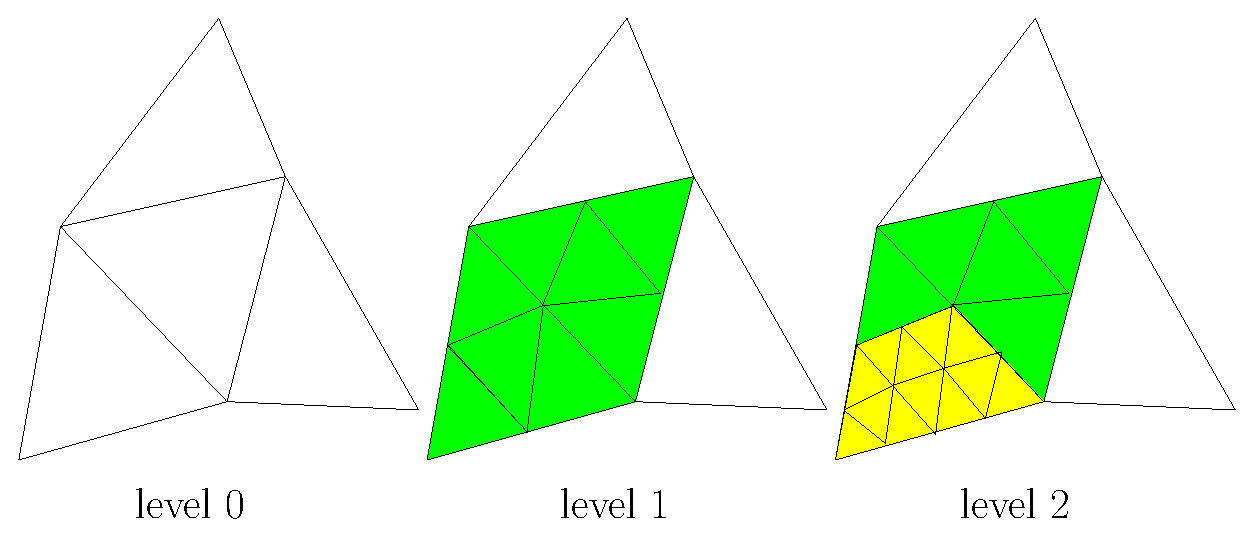
\includegraphics[width=0.9\textwidth]{refinement-levels2}
\par\end{centering}

\caption{\label{fig:Refinement-levels}Refinement levels}


\end{figure}


Identifying triangles for refinement is done using a residual-based
error estimation method \cite[Chap.~9]{bs:mtfem}. If the problem
is to solve $\mathcal{L}u=b$ where $\mathcal{L}$ is a linear differential
operator $V\to V'$, $V$ a Hilbert space (typically a Sobolev space),
then we need to estimate the norm of $\mathcal{L}u-b$ in $V'$ (the
dual space of $V$). This in turn involves estimating 
\[
\sup_{w\in V}\frac{\left\langle \mathcal{L}u-b,\, w\right\rangle _{V\times V'}}{\left\Vert w\right\Vert _{V}}.
\]
Since differential operators are local operators (that is, if $u(\mathbf{x})=v(\mathbf{x})$
for all $\mathbf{x}$ near $\mathbf{x}^{*}$, then $\mathcal{L}u(\mathbf{x}^{*})=\mathcal{L}v(\mathbf{x}^{*})$),
this residual can be estimated on each element and its boundary. If
$V_{h}$ is the finite element space (generated by all basis functions
over all elements in the triangulation), then the Galerkin method
already implies that $\left\langle \mathcal{L}u-b,\, w\right\rangle _{V\times V'}=0$
for all $w\in V_{h}$. So we need to go beyond just the basis functions
of $V_{h}$ in order to estimate the error in the solution. For the
problem
\begin{eqnarray*}
-\nabla\cdot\left(\alpha\nabla u\right) & = & f\qquad\mbox{in }\Omega,\\
u & = & g\qquad\mbox{on }\partial\Omega,
\end{eqnarray*}
for example, \cite[Chap.~9]{bs:mtfem} develops the \emph{a posteriori}
residual estimate 
\[
\left\Vert e_{h}\right\Vert _{H^{-1}(\Omega)}\leq\mbox{constant}\,\left[\sum_{K}\left\Vert \nabla\cdot\left(\alpha\nabla u_{h}\right)+f\right\Vert _{L^{2}(K)}^{2}h_{K}^{2}+\sum_{e}\left\Vert \left[\alpha\mathbf{n}\cdot\nabla u_{h}\right]_{\mathbf{n}}\right\Vert _{L^{2}(e)}^{2}h_{e}\right]^{1/2}
\]
where $K$ ranges over all triangles in the triangulation, and $e$
ranges over all edges in the triangulation in the interior of the
domain $\Omega$. The quantity $\left[\alpha\mathbf{n}\cdot\nabla u_{h}\right]_{\mathbf{n}}$
is the jump in the value of $\alpha\mathbf{n}\cdot\nabla u_{h}$ between
the values in the two elements incident to the edge $e$; $\mathbf{n}$
is the unit normal vector to the edge $e$. Note that it does not
matter which sign is chosen for $\mathbf{n}$ in determining $\left\Vert \left[\alpha\mathbf{n}\cdot\nabla u_{h}\right]_{\mathbf{n}}\right\Vert _{L^{2}(e)}^{2}$.
Also note that $h_{K}$ is the diameter of triangle $K$, which is
equal to the length of the longest edge; $h_{e}$ is the length of
edge $e$. 

For a triangle $K$ in the triangulation, we can use 
\[
\left[\left\Vert \nabla\cdot\left(\alpha\nabla u_{h}\right)+f\right\Vert _{L^{2}(K)}^{2}h_{K}^{2}+\sum_{e}\left\Vert \left[\alpha\mathbf{n}\cdot\nabla u_{h}\right]_{\mathbf{n}}\right\Vert _{L^{2}(e)}^{2}h_{e}\right]^{1/2}
\]
where $e$ ranges over the edges of $K$ as an estimate of the error
due to the triangle $K$. If this exceeds a threshold, then that triangle
should be marked for refinement. Since the basis functions of refined
triangles associated with the common boundary between refined and
unrefined triangles must be made ``slaves'' to the basis functions
on the adjacent unrefined triangles, we should create an additional
``buffer'' region of refined triangles. Thus: a triangle should
also be refined if it is adjacent to a triangle with an excessively
large error estimate.


\subsection{Representation of refined mesh}

The refinement of a single element is represented by the standard
refinement, which is a triangulation of the reference element (\texttt{p\_refref},\texttt{t\_refref})
(here ``refref'' indicates ``reference element refinement''),
being the points and triangles of the triangulation in the manner
of (\texttt{p},\texttt{t}) described above. We need a data structure
similar to that for element types: in order to join refined triangles
from different master triangles, we need to associate a unique geometric
feature of the master triangle to each node of the refinement. We
also need to identify permuations of nodes that occur due to the permutations
of the geometric features. These should work very much like \texttt{pxfeature()},
\texttt{nvars} and \texttt{flist} in the element type data structures.
(Here we replace \texttt{nvars} with \texttt{npts}.) This will give
us a ``refref'' or ``reference element refinement'' data structure.
An example reference refinement is shown in Figure~\ref{fig:Reference-refinement-example}.
Note that for this reference refinement using piecewise linear element
(\texttt{lin2d\_elt()}) we have
\[
B=\left[\begin{array}{cccccc}
1 &  &  &  & 1/2 & 1/2\\
 & 1 &  & 1/2 &  & 1/2\\
 &  & 1 & 1/2 & 1/2
\end{array}\right].
\]


\begin{figure}
\noindent \begin{centering}
\includegraphics[width=0.45\textwidth]{refref1}
\par\end{centering}

\caption{\label{fig:Reference-refinement-example}Reference refinement example}


\end{figure}


\nwenddocs{}\nwbegincode{206}\sublabel{NWpdeB-refS-1}\nwmargintag{{\nwtagstyle{}\subpageref{NWpdeB-refS-1}}}\moddef{reference refinement example~{\nwtagstyle{}\subpageref{NWpdeB-refS-1}}}\endmoddef
p_refref = [0 0; 1 0; 0 1; 1/2 1/2; 0 1/2; 1/2 0];
t_refref = [1 5 6; 2 4 6; 3 4 5; 4 5 6];
npts     = [1;     1;     1;     1;     1;     1];  % number of points in each geometric feature
flist    = [1 0 0; 2 0 0; 3 0 0; 2 3 0; 1 3 0; 1 2 0];
Brefref  = [1 0 0   0 1/2 1/2;
            0 1 0 1/2   0 1/2;
            0 0 1 1/2 1/2   0];
refref2d = struct('p',p_refref,'t',t_refref,'npts',npts,'flist',flist, ...
                     'Brefref',Brefref,'pxfeature',@px_refref1);
\nwnotused{reference\ refinement\ example}\nwendcode{}\nwbegindocs{207}\nwdocspar

Note that the points in \texttt{p\_refref} must occur in the order
described by \texttt{flist} and \texttt{npts}. Also, if a vertex of
the reference refinement is also a vertex of the reference element,
then there can only be one point associated with that geometric feature:
if \texttt{flist(k,:)} represents a vertex (of the reference element),
then \texttt{npts(k)} must be one.

The relationship between the basis functions on the reference element,
and the basis functions on the standard refinement is given by the
$\left[b_{ij}\right]$ matrix \texttt{B\_refref}. The indexes into
this matrix is given by the standard ordering of basis functions as
defined by \texttt{Aphihat()} for $i$, but for $j$ we can use the
basis function numbers assigned by \texttt{create\_fht()}. 

A test mesh for applying the refinement to is shown in Figure~\ref{fig:Test-mesh-refinement}.
The dashed lines show the refined mesh. The triangulation of this
test mesh is given below.

\nwenddocs{}\nwbegincode{208}\sublabel{NWpdeB-refT-1}\nwmargintag{{\nwtagstyle{}\subpageref{NWpdeB-refT-1}}}\moddef{refinement test triangulation~{\nwtagstyle{}\subpageref{NWpdeB-refT-1}}}\endmoddef
p_testref = [0 0; 1.5 0; 2.5 0; 3.5 0; 3.5 1; ...
    2.5 0.7; 1.5 1; 0 1; 1.5 2; 2.5 1.5];
t_testref = [1 2 7; 2 7 6; 2 3 6; 4 3 6; 4 5 6; ...
    10 5 6; 6 10 7; 1 7 8; 8 7 9; 7 9 10];
\nwnotused{refinement\ test\ triangulation}\nwendcode{}\nwbegindocs{209}\nwdocspar

\begin{figure}
\noindent \begin{centering}
\includegraphics[width=0.7\textwidth]{test-ref-grid}
\par\end{centering}

\caption{\label{fig:Test-mesh-refinement}Test mesh for refinement}


\end{figure}



\subsection{Generating refined meshes}

The algorithm to create the refined mesh basically involves processing
each triangle in the ``master triangulation''. We process each geometric
feature of each master triangle using an initially empty hash table
of geometric features (\texttt{rfht}). For each geometric feature
that is not in the hash table, and is not a vertex, we create new
points according to the points associated with that geometric feature
of the reference refinement. The geometric feature is then added as
a key to the hash table; the value of the key in the table is the
ordered list of point indexes in the refined triangulation. For each
master triangle to be refined, we need to create a map (\texttt{p\_rr\_trx})
that translates point indexes in the reference refinement into point
indexes in the actual refined mesh. The points in the reference refinement
must be transformed to actual points in the refined mesh (this involves
the transformation $\widehat{\mathbf{x}}\mapsto T\widehat{\mathbf{x}}+\mathbf{b}=\mathbf{x}$. 

\nwenddocs{}\nwbegincode{210}\sublabel{NWpdeB-fil8-X}\nwmargintag{{\nwtagstyle{}\subpageref{NWpdeB-fil8-X}}}\moddef{filelist~{\nwtagstyle{}\subpageref{NWpdeB-fil8-1}}}\plusendmoddef
create-refinement.m \\
\nwendcode{}\nwbegincode{211}\sublabel{NWpdeB-creJ-1}\nwmargintag{{\nwtagstyle{}\subpageref{NWpdeB-creJ-1}}}\moddef{create-refinement.m~{\nwtagstyle{}\subpageref{NWpdeB-creJ-1}}}\endmoddef
function [p_ref,t_ref,master_ref,idx_ref,rfht,master2rr_pt] = ...
create_refinement(p,t,refine_list,refref)
% function [p_ref,t_ref,master_ref,idx_ref,rfht,master2rr_pt] = ...
% create_refinement(p,t,refine_list,refref)
%
% Create refined mesh using reference refinement refref.
% (p,t) represent the unrefined "master" triangulation,
% where refine_list is the list of triangle indexes that are
% to be refined: the triangles to be refined are
% t(refine_list(i),:), i = 1, ..., length(refine_list).
% The returned items are:
% (p_ref,t_ref) are the triangulation of the refined mesh
% master_ref(i) is the row index into t of the master triangle
% of triangle t_ref(i,:)
% idx_ref(i) is the row index into refref.t identifies
% which sub-triangle of triangle master_ref(i) is t_ref(i,:).
% Note that idx_ref(i) == 0 iff t_ref(i,:) is an unrefined triangle.
%
% master2rr_pt(i,:) is the ordered list of indexes of points in
% master triangle i that are in the refined mesh.
% master2rr_pt(i,j) is the index into p_ref of master triangle i
% and point refref.p(j,:).

np = size(p,1);
rfht = containers.Map('KeyType','int64','ValueType','any');
rr_npts = refref.npts;
rr_flist = refref.flist;
p_ref = p; % include all points of unrefined triangles
t_ref = [];
master_ref = [];
nt_ref = 0;
np_ref = size(p,1);
ismaster = zeros(size(t,1),1);
ismaster(refine_list) = 1;
master2rr_pt = zeros(size(t,1),size(refref.p,1));
p_rr_trx = zeros(size(refref.p,1),1);
idx_ref = [];
for i = 1:size(t,1)
    % master_triangle_i = t(i,:)
    % master_triangle_points = [p(t(i,1),:); p(t(i,2),:); p(t(i,3),:)] 
    p_rr_trx(:) = 0;
    if ismaster(i)
        % vertices of master triangle
        p1 = p(t(i,1),:); p2 = p(t(i,2),:); p3 = p(t(i,3),:);
        % transformation from ref element to master triangle
        T = [p2'-p1', p3'-p1'];
        b = p1';
        % transform points in reference refinement
        % Tp_rr = zeros(size(refref.p));
        % for j = 1:size(refref.p,1)
        % Tp_rr(j,:) = refref.p(j,:)*T' + b';
        % end
        Tp_rr = bsxfun(@plus,refref.p*T',b');
        p_rr_idx = 1; % index into refref.p
        % for each geometric feature of the master triangle ...
        for k = 1:size(rr_flist,1) 
            npts_k = refref.npts(k);
            if length(find(rr_flist(k,:))) ~= 1 % not a vertex
                % if geometric feature not in hash table, add the points
                f = rr_flist(k,:);
                f = f(find(f));
                [f,px] = sort(t(i,f));
                fref = get_feature_ref(f,np);
                pt_px = refref.pxfeature(px);
                if ~ isKey(rfht,fref)
                    pt_list = np_ref + (1:npts_k);
                    rfht(fref) = pt_list;
                    p_ref = [p_ref; Tp_rr(p_rr_idx-1+pt_px,:)];
                    np_ref = np_ref + npts_k;
                else % isKey(rfht,fref)
                    pt_list = rfht(fref);
                end % if
                p_rr_trx(p_rr_idx-1+(1:npts_k)) = pt_list(pt_px);
            else   % is a vertex of a master triangle, so use the corresponding 
                % vertex of the master triangle
                p_rr_trx(p_rr_idx) = t(i,rr_flist(k,1));
            end % if
            p_rr_idx = p_rr_idx + npts_k;
        end % for k
        % p_rr_trx
        % refined_points = p_ref(p_rr_trx,:)
        % now add the refined triangles to the mesh
        % new_t_ref = p_rr_trx(refref.t)
        t_ref = [t_ref; p_rr_trx(refref.t)];
        idx_ref = [idx_ref; (1:size(refref.t,1))'];
        nt_ref = nt_ref + size(refref.t,1);
        master_ref = [master_ref, i*ones(1,size(refref.t,1))];
        master2rr_pt(i,:) = p_rr_trx'; % turn p_rr_trx into row vector
    else % ~ ismaster(i)
        % no extra points, just one extra triangle
        nt_ref = nt_ref + 1;
        t_ref = [t_ref; t(i,:)];
        master_ref(nt_ref) = i;
        idx_ref(nt_ref) = 0; % not a refined triangle
        master2rr_pt(i,1:3) = t(i,:);
    end % if ismaster(i)
end % for i
\nwnotused{create-refinement.m}\nwendcode{}\nwbegindocs{212}\nwdocspar

Test code for \texttt{create\_refinement()} follows. The reference
refinements for these tests are firstly a simple subdivision of the
reference element into four congruent sub-triangles. The second subdivides
each edge into thirds, resulting in a subdivision into 10 congruent
sub-triangles. The third reference refinement included a sub-triangle
that is completely contained within the interior of the reference
element. This was used to check that the ordering of the vertices
did not cause incorrect refinements.

\nwenddocs{}\nwbegincode{213}\sublabel{NWpdeB-fil8-Y}\nwmargintag{{\nwtagstyle{}\subpageref{NWpdeB-fil8-Y}}}\moddef{filelist~{\nwtagstyle{}\subpageref{NWpdeB-fil8-1}}}\plusendmoddef
ref-test-script.m \\
\nwendcode{}\nwbegincode{214}\sublabel{NWpdeB-refH-1}\nwmargintag{{\nwtagstyle{}\subpageref{NWpdeB-refH-1}}}\moddef{ref-test-script.m~{\nwtagstyle{}\subpageref{NWpdeB-refH-1}}}\endmoddef
% Test script for refinement
p_refref = [0 0; 1 0; 0 1; 1/2 1/2; 0 1/2; 1/2 0];
t_refref = [1 5 6; 2 4 6; 3 4 5; 4 5 6];
npts = [1; 1; 1; 1; 1; 1];
flist = [1 0 0; 2 0 0; 3 0 0; 2 3 0; 1 3 0; 1 2 0];
Brefref = [1 0 0 0 1/2 1/2;
0 1 0 1/2 0 1/2;
0 0 1 1/2 1/2 0];
px_refref1 = @(px)[1];
refref2d = struct('p',p_refref,'t',t_refref,'npts',npts,'flist',flist, ...
'Brefref',Brefref,'pxfeature',px_refref1);
p_testref = [0 0; 1.5 0; 2.5 0; 3.5 0; 3.5 1; ...
2.5 0.7; 1.5 1; 0 1; 1.5 2; 2.5 1.5];
t_testref = [1 2 7; 2 7 6; 2 3 6; 4 3 6; 4 5 6; ...
10 5 6; 6 10 7; 1 7 8; 8 7 9; 7 9 10];
trimesh(t_testref,p_testref(:,1),p_testref(:,2))
axis([-.3 4 -.3 3])
master = [1,2,3,4,5,7,8]
[p_ref,t_ref,master_ref,idx_refref,rfht] = ...
create_refinement(p_testref,t_testref,master,refref2d)
trimesh(t_ref,p_ref(:,1),p_ref(:,2))
'Press any key to continue'
pause

p_refref2 = [0 0; 1 0; 0 1; 2/3 1/3; 1/3 2/3; 0 1/3; 0 2/3; 1/3 0; 2/3 0; 1/3 1/3];
t_refref2 = [1 8 6; 6 8 10; 8 9 10; 9 4 10; 9 2 4; 7 6 10; 10 5 7; 10 4 5; 7 5 3];
npts2 = [ 1; 1; 1; 2; 2; 2; 1];
flist2 = [1 0 0; 2 0 0; 3 0 0; 2 3 0; 1 3 0; 1 2 0; 1 2 3];
px_refref2 = @(px)ifte(length(px)==2,px,[1])
refref2d_2 = struct('p',p_refref2,'t',t_refref2,'npts',npts2,'flist',flist2, ...
'Brefref',[],'pxfeature',px_refref2);
[p_ref2,t_ref2,master_ref2,idx_refref2,rfht2] = ...
create_refinement(p_testref,t_testref,master,refref2d_2)
trimesh(t_ref2,p_ref2(:,1),p_ref2(:,2))
'Press any key to continue'
pause

npts3 = [ 1; 1; 1; 1; 1; 1; 3];
flist3 = [1 0 0; 2 0 0; 3 0 0; 2 3 0; 1 3 0; 1 2 0; 1 2 3];
p_refref3 = [0 0; 1 0; 0 1; 1/2 1/2; 0 1/2; 1/2 0; 1/6 1/6; 2/3 1/6; 1/6 2/3];
t_refref3 = [1 7 6; 6 7 8; 6 8 2; 7 5 1; 7 5 9; 7 8 9; 8 9 4; 2 4 8; 5 9 3; 9 4 3];
size_p_refref3 = size(p_refref3)
size_t_refref3 = size(t_refref3)
px_refref3 = @(px)ifte(length(px)==3,px,[1])
refref2d_3 = struct('p',p_refref3,'t',t_refref3,'npts',npts3,'flist',flist3, ...
'Brefref',[],'pxfeature',px_refref3)
[p_ref3,t_ref3,master_ref3,idx_refref3,rfht3] = ...
create_refinement(p_testref,t_testref,master,refref2d_3)
trimesh(t_ref3,p_ref3(:,1),p_ref3(:,2))
\nwnotused{ref-test-script.m}\nwendcode{}\nwbegindocs{215}\nwdocspar


\subsubsection{Finding the internal boundary between refined and unrefined elements}

The next task is to determine the edges (or faces in 3-D) common to
both the unrefined and refined master triangles. The main idea is
to find all edges of triangles that appear exactly once in both the
refined and unrefined sets of triangles, but appear exactly twice
in the union of these sets of edges.

\nwenddocs{}\nwbegincode{216}\sublabel{NWpdeB-fil8-Z}\nwmargintag{{\nwtagstyle{}\subpageref{NWpdeB-fil8-Z}}}\moddef{filelist~{\nwtagstyle{}\subpageref{NWpdeB-fil8-1}}}\plusendmoddef
get-internal-boundary2d.m \\
\nwendcode{}\nwbegincode{217}\sublabel{NWpdeB-getP-1}\nwmargintag{{\nwtagstyle{}\subpageref{NWpdeB-getP-1}}}\moddef{get-internal-boundary2d.m~{\nwtagstyle{}\subpageref{NWpdeB-getP-1}}}\endmoddef
function [bedges,bnodes,t_idx1,t_idx2] = get_internal_boundary2d(t,t_list)
% function [bedges,bnodes,t_idx1,t_idx2] = get_internal_boundary2d(t,t_list)
%
% Returns the boundary between the triangles in t_list and its complement.
% t_list is a list of row indexes i into t(i,j)
% bedges is an m x 2 array listing the edges in the boundary.
% bnodes is a  p x 1 array listing the nodes in the boundary.
% t_idx1(i) is the triangle containing bedges(i) in t_list.
% t_idx2(i) is the triangle containing bedges(i) in the complement of t_list.
t_list = t_list';
% compute complement of t_list
tf = zeros(size(t,1),1);
tf(t_list) = 1;
ct_list = find(tf == 0);
% compute boundary of each part ...
[bedges1,bnodes1,t_idx1a] = boundary2d(t( t_list,:));
[bedges2,bnodes2,t_idx2a] = boundary2d(t(ct_list,:));
% ... and find the common part
temp = sortrows([bedges1, t_list(t_idx1a); 
                 bedges2,ct_list(t_idx2a)+size(t,1)]);
[temp2,idx1] = unique(temp(:,1:2),'rows','first');
[temp2,idx2] = unique(temp(:,1:2),'rows','last');
difflist = find(idx1 ~= idx2);
bedges = temp(idx1(difflist),1:2);
t_idx1 = temp(idx1(difflist),3)';
t_idx2 = temp(idx2(difflist),3)' - size(t,1);
bnodes = unique(sort(bedges(:)));
\nwnotused{get-internal-boundary2d.m}\nwendcode{}\nwbegindocs{218}\nwdocspar


\subsubsection{Getting the edges of the reference refinement corresponding to an
edge of the reference triangle}

This only needs to be computed once for each edge of the reference
triangle.

\nwenddocs{}\nwbegincode{219}\sublabel{NWpdeB-fil8-a}\nwmargintag{{\nwtagstyle{}\subpageref{NWpdeB-fil8-a}}}\moddef{filelist~{\nwtagstyle{}\subpageref{NWpdeB-fil8-1}}}\plusendmoddef
rr-get-redges.m \\
\nwendcode{}\nwbegincode{220}\sublabel{NWpdeB-rr*F-1}\nwmargintag{{\nwtagstyle{}\subpageref{NWpdeB-rr*F-1}}}\moddef{rr-get-redges.m~{\nwtagstyle{}\subpageref{NWpdeB-rr*F-1}}}\endmoddef
function [elist,rrtlist] = rr_get_redges(edge,rr) 
% function [elist,rrtlist] = rr_get_redges(edge,rr) 
% 
% Return list of refined edges in edge in the 
% reference refinement.  Note that edge % is a pair of indexes into rr.p for the 
% reference triangle. 0; 
% First find list of points in refined triangulation 
% in edge from master triangulation. 
ptlist = []; 
npts  = rr.npts; 
cnpts = cumsum(rr.npts); 
for k = 1:size(rr.flist,1)
    f = rr.flist(k,:);
    f = f(find(f));
    idx = subset_scan(f,edge);
    if min(idx) > 0 % then f is a subset of edge
        ptlist = [ptlist, (cnpts(k)-npts(k)+1):cnpts(k)];
    end 
end 
% ptlist 
% Now find edges in reference refinement that are 
% in edge in the master triangulation 
elist = []; 
rrtlist = []; 
for i = 1:size(rr.t)
    % triangle = rr.t(i,:)
    idx = subset_scan(rr.t(i,:),ptlist);
    if sum(idx > 0) == 2
        % 2 of the 3 vertices are in ptlist
        elist = [elist; rr.t(i,find(idx>0))];
        rrtlist = [rrtlist, i];
    end 
end 
elist = sort(elist,2); 
\nwnotused{rr-get-redges.m}\nwendcode{}\nwbegindocs{221}\nwdocspar


\subsubsection{Creating the stiffness matrices for adapted meshes}

To create the stiffness matrices we use the assumption that the basis
functions on the reference element can be expressed as linear combinations
of the basis functions on the reference refinement. The $B$ matrix
gives the relationship between the basis functions on the reference
element ($\widehat{\phi}_{i}$) and the basis functions on the reference
refinement ($\widetilde{\phi}_{j}$):
\[
\widehat{\phi}_{i}=\sum_{j}b_{ij}\widetilde{\phi}_{j}.
\]
This matrix depends both on the reference refinement and the element
type. This can be computed as follows for piecewise linear elements:

\nwenddocs{}\nwbegincode{222}\sublabel{NWpdeB-calP-1}\nwmargintag{{\nwtagstyle{}\subpageref{NWpdeB-calP-1}}}\moddef{calculation of $B$ matrix~{\nwtagstyle{}\subpageref{NWpdeB-calP-1}}}\endmoddef
lin2d = lin2d_elt()
[fht_rr,v2tnum_rr,v2fnum_rr,v2fidx_rr] = ...
    create_fht(refref2d.p,refref2d.t,lin2d)
nvars = fht_num_vars(fht_rr)
ls_rr = struct('coeffs',@(x)1,'rhs',@(x)lin2d.Aphihat(x,0)', ...
    'order',0)
A = zeros(nvars,nvars);
b = zeros(nvars,sum(lin2d.nvars));
[A,b] = assembly2d(A,b,ls_rr,lin2d,refref2d.p,refref2d.t, ...
    fht_rr,@int2d_radon7)
Brefref = A \\ b;
\nwnotused{calculation\ of\ {\char36}B{\char36}\ matrix}\nwendcode{}\nwbegindocs{223}\nwdocspar

The next step is to determine the edges of the sub-triangles that
are part of the internal boundary between refined and unrefined triangles.
We use a utility routine \texttt{subset\_scan()} defined below.

\nwenddocs{}\nwbegincode{224}\sublabel{NWpdeB-fil8-b}\nwmargintag{{\nwtagstyle{}\subpageref{NWpdeB-fil8-b}}}\moddef{filelist~{\nwtagstyle{}\subpageref{NWpdeB-fil8-1}}}\plusendmoddef
subset-scan.m \\
\nwendcode{}\nwbegincode{225}\sublabel{NWpdeB-subD-1}\nwmargintag{{\nwtagstyle{}\subpageref{NWpdeB-subD-1}}}\moddef{subset-scan.m~{\nwtagstyle{}\subpageref{NWpdeB-subD-1}}}\endmoddef
function idx = subset_scan(list1,list2)
% function idx = subset_scan(list1,list2)
%
% Returns index list idx where
% if idx(i) != 0 then list1(i) == list2(idx(i)), and
% if idx(i) == 0 then list1(i) ~= list2(j) for any j.
idx = zeros(size(list1));
[list1,px1] = sort(list1);
[list2,px2] = sort(list2);
i1 = 1;
i2 = 1;
while i1 <= length(list1) && i2 <= length(list2)
    if list1(i1) < list2(i2)
        i1 = i1 + 1;
    elseif list1(i1) > list2(i2)
        i2 = i2 + 1;
    else
        idx(px1(i1)) = px2(i2);
        i1 = i1 + 1;
        i2 = i2 + 1;
    end
end
\nwnotused{subset-scan.m}\nwendcode{}\nwbegincode{226}\sublabel{NWpdeB-genv-1}\nwmargintag{{\nwtagstyle{}\subpageref{NWpdeB-genv-1}}}\moddef{generate hash table of point lists for geometric features~{\nwtagstyle{}\subpageref{NWpdeB-genv-1}}}\endmoddef
\nwnotused{generate\ hash\ table\ of\ point\ lists\ for\ geometric\ features}\nwendcode{}\nwbegincode{227}\sublabel{NWpdeB-finZ-1}\nwmargintag{{\nwtagstyle{}\subpageref{NWpdeB-finZ-1}}}\moddef{find edges of refined sub-triangles~{\nwtagstyle{}\subpageref{NWpdeB-finZ-1}}}\endmoddef
\nwnotused{find\ edges\ of\ refined\ sub-triangles}\nwendcode{}\nwbegindocs{228}\nwdocspar


\subsection{Combining multiple levels of refinement in matrix assembly}


\subsection{Error estimation and identification of triangles to refine}


\section{\label{sec:Output-and-visualization}Output and visualization}


\subsection{\label{sub:Visualization}Visualization\index{visualization}}

Visualization of the results is greatly simplified by Matlab's \texttt{\index{trimesh()}trimesh()}
function. For example, to see a triangulation as given by (\texttt{p},\texttt{t}),
we use

\nwenddocs{}\nwbegincode{229}\sublabel{NWpdeB-triF-1}\nwmargintag{{\nwtagstyle{}\subpageref{NWpdeB-triF-1}}}\moddef{trimesh-example~{\nwtagstyle{}\subpageref{NWpdeB-triF-1}}}\endmoddef
trimesh(t,p(:,1),p(:,2))
\nwnotused{trimesh-example}\nwendcode{}\nwbegindocs{230}\nwdocspar


\subsubsection{\label{sub:Visualizing-solutions}Visualizing solutions (and mesh
functions)}

One way of seeing the solution of a PDE (or some other quantity defined
on a mesh for a certain element) is to get the list of variables associated
with each point and plot those variable values. This will work for
scalar element types of Lagrange type (such as the piecewise linear,
quadratic, and cubic elements described in Sections~\ref{sub:Piecewise-linear-elements},
\ref{sub:Piecewise-quadratic-elements}, and \ref{sub:Piecewise-cubic-elements}).
We can use the following routine:\index{get_pvlist()@\texttt{get\_pvlist()}}

\nwenddocs{}\nwbegincode{231}\sublabel{NWpdeB-fil8-c}\nwmargintag{{\nwtagstyle{}\subpageref{NWpdeB-fil8-c}}}\moddef{filelist~{\nwtagstyle{}\subpageref{NWpdeB-fil8-1}}}\plusendmoddef
get-pvlist.m \\
\nwendcode{}\nwbegincode{232}\sublabel{NWpdeB-getC-1}\nwmargintag{{\nwtagstyle{}\subpageref{NWpdeB-getC-1}}}\moddef{get-pvlist.m~{\nwtagstyle{}\subpageref{NWpdeB-getC-1}}}\endmoddef
function pvlist = get_pvlist(fht,np)
% function pvlist = get_pvlist(fht,np)
%
% Get list of variable indexes for the points.
% That is, pvlist(i) is the variable number for the point
% in the triangulation with index i.
% As usual, np is the number of points.
pvlist = zeros(np,1);
for i = 1:np
    pvlist(i) = fht(get_feature_ref(i,np));
end
\nwnotused{get-pvlist.m}\nwendcode{}\nwbegindocs{233}\nwdocspar

Then we can view the solution via

\nwenddocs{}\nwbegincode{234}\sublabel{NWpdeB-visL-1}\nwmargintag{{\nwtagstyle{}\subpageref{NWpdeB-visL-1}}}\moddef{visualization-example~{\nwtagstyle{}\subpageref{NWpdeB-visL-1}}}\endmoddef
u = ...;  % compute solution
np = size(p,1);
pvlist = get_pvlist(fht,np); 
trimesh(t,p(:,1),p(:,2),u(pvlist)) 
\nwnotused{visualization-example}\nwendcode{}\nwbegindocs{235}\nwdocspar


\subsubsection{\label{sub:Boundary-visualization}Boundary visualization}

There are two functions for boundary visualization: one which plots
just the boundary and one with the boundary and normal vectors.\index{plot_boundary2d()@\texttt{plot\_boundary2d()}}

\nwenddocs{}\nwbegincode{236}\sublabel{NWpdeB-fil8-d}\nwmargintag{{\nwtagstyle{}\subpageref{NWpdeB-fil8-d}}}\moddef{filelist~{\nwtagstyle{}\subpageref{NWpdeB-fil8-1}}}\plusendmoddef
plot-boundary2d.m \\
\nwendcode{}\nwbegincode{237}\sublabel{NWpdeB-ploH-1}\nwmargintag{{\nwtagstyle{}\subpageref{NWpdeB-ploH-1}}}\moddef{plot-boundary2d.m~{\nwtagstyle{}\subpageref{NWpdeB-ploH-1}}}\endmoddef
function plot_boundary2d(p,t,bb)
% function plot_boundary2d(p,t,bb)
%
% Plots the boundary of a mesh in 2D given by p and t.
% The i'th point is p(i,:), and triangle j is given by
% points with indexes t(j,1), t(j,2) & t(j,3).
%
% The bounding box is given in bb = [xmin, xmax, ymin,ymax].
%
% See distmesh.m etc.
[bedges,bnodes] = boundary2d(t);
bdry_tri = [bedges(:,1),bedges(:,2),bedges(:,2)];
triplot(bdry_tri,p(:,1),p(:,2));
axis(bb)
\nwnotused{plot-boundary2d.m}\nwendcode{}\nwbegindocs{238}\nwdocspar

And now with normal vectors (use with equal axes to preserve orthogonality):\index{plot_boundary2dwnormals()@\texttt{plot\_boundary2dwnormals()}}

\nwenddocs{}\nwbegincode{239}\sublabel{NWpdeB-fil8-e}\nwmargintag{{\nwtagstyle{}\subpageref{NWpdeB-fil8-e}}}\moddef{filelist~{\nwtagstyle{}\subpageref{NWpdeB-fil8-1}}}\plusendmoddef
plot-boundary2dwnormals.m \\
\nwendcode{}\nwbegincode{240}\sublabel{NWpdeB-ploP-1}\nwmargintag{{\nwtagstyle{}\subpageref{NWpdeB-ploP-1}}}\moddef{plot-boundary2dwnormals.m~{\nwtagstyle{}\subpageref{NWpdeB-ploP-1}}}\endmoddef
function plot_boundary2dwnormals(p,t,bb)
% function plot_boundary2dwnormals(p,t,bb)
%
% Plots the boundary of a mesh in 2D given by p and t.
% The i'th point is p(i,:), and triangle j is given by
% points with indexes t(j,1), t(j,2) & t(j,3).
% The normals are also plotted from the center of each edge.
% The length of the normal vectors is the length of the edge.
%
% The bounding box is given in bb = [xmin, xmax, ymin,ymax].
%
% See distmesh.m etc.
[bedges,bnodes,normals] = boundary2d_2(p,t);
bdry_tri = [bedges(:,1),bedges(:,2),bedges(:,2)];
midpts = 0.5*(p(bedges(:,1),:)+p(bedges(:,2),:));
len_edges = sqrt(sum((p(bedges(:,1),:)-p(bedges(:,2),:)).^2,2));
arrowpts = midpts + diag(sparse(len_edges))*normals;
hold on
triplot(bdry_tri,p(:,1),p(:,2));
arrow(midpts,arrowpts);
axis(bb);
hold off
\nwnotused{plot-boundary2dwnormals.m}\nwendcode{}\nwbegindocs{241}\nwdocspar


\subsubsection{Labelled meshes in two dimensions}

While \texttt{trimesh()} is very convenient for showing a triangulation,
often we need vertex labels as well. The following code does this.

\nwenddocs{}\nwbegincode{242}\sublabel{NWpdeB-fil8-f}\nwmargintag{{\nwtagstyle{}\subpageref{NWpdeB-fil8-f}}}\moddef{filelist~{\nwtagstyle{}\subpageref{NWpdeB-fil8-1}}}\plusendmoddef
trimesh-labelled.m \\
\nwendcode{}\nwbegincode{243}\sublabel{NWpdeB-triI-1}\nwmargintag{{\nwtagstyle{}\subpageref{NWpdeB-triI-1}}}\moddef{trimesh-labelled.m~{\nwtagstyle{}\subpageref{NWpdeB-triI-1}}}\endmoddef
function trimesh_labelled(p,t)
% function trimesh_labelled(p,t)
%
% Produces plot of triangulation, labelled by vertex number
trimesh(t,p(:,1),p(:,2));
for i = 1:size(p,1)
    text(p(i,1),p(i,2),num2str(i));
end
\nwnotused{trimesh-labelled.m}\nwendcode{}\nwbegindocs{244}\nwdocspar


\subsection{\label{sub:Refined-output}Refined output}

The results of \texttt{\index{trimesh()}trimesh()} do not capture
the higher order behavior of the mesh function or solution as it assumes
the function is piecewise linear. To capture the quadratic or higher
order behavior we need to create a sub-mesh and plot on the submesh.
This can be done by, for example, creating a sub-mesh for the reference
element, and then replacing each triangle in the triangulation with
the reference element's sub-mesh transformed in the usual way ($\widehat{\mathbf{x}}\mapsto\mathbf{x}=T_{K}\widehat{\mathbf{x}}+\mathbf{b}_{K}$).
The values can then be computed on the sub-mesh of the original triangulation,
and the result plotted using \texttt{trimesh()}.

First we have code to create a sub-mesh for the reference element.\index{ref_triangle_submesh()@\texttt{ref\_triangle\_submesh()}}

\nwenddocs{}\nwbegincode{245}\sublabel{NWpdeB-fil8-g}\nwmargintag{{\nwtagstyle{}\subpageref{NWpdeB-fil8-g}}}\moddef{filelist~{\nwtagstyle{}\subpageref{NWpdeB-fil8-1}}}\plusendmoddef
ref-triangle-submesh.m \\
\nwendcode{}\nwbegincode{246}\sublabel{NWpdeB-refM-1}\nwmargintag{{\nwtagstyle{}\subpageref{NWpdeB-refM-1}}}\moddef{ref-triangle-submesh.m~{\nwtagstyle{}\subpageref{NWpdeB-refM-1}}}\endmoddef
function [p,t] = ref_triangle_submesh(n)
% function [p,t] = ref_triangle_submesh(n)
%
% Creates a standard mesh on the reference triangle
% (vertices at (0,0), (1,0) and (0,1)).
% n+1 is the number of grid points on each edge
% Generate points
p = zeros(n*(n+1)/2,2);
k = 1;
for i = 0:n
    for j = 0:n-i
        p(k,:) = [i,j];
        k = k+1;
    end
end
p = p / n;
% Create triangulation
t = zeros(n*n,3);
k = 1;
idx = 1;
for i = 0:n-1
    for j = 0:n-i-1
        if j > 0
            t(k,:) = [idx, idx+n-i, idx+n-i+1];
            k = k+1;
        end
        t(k,:) = [idx, idx+n-i+1, idx+1];
        k = k+1;
        idx = idx+1;
    end % for j
    idx = idx+1;
end % for i
\nwnotused{ref-triangle-submesh.m}\nwendcode{}\nwbegindocs{247}\nwdocspar

Once a sub-mesh for the reference element has been created, the creation
of the sub-mesh of the original triangulation, and the computation
of the values at the sub-mesh nodes, is handled by the following code.
Let $g(\mathbf{x})$ be the mesh-based function represented by the
values of \texttt{vars}. Then \texttt{vals(i,1)} contains $g(\widetilde{\mathbf{x}}_{i})$
where $\widetilde{\mathbf{x}}_{i}$ where $\widetilde{\mathbf{x}}_{i}$
is point $i$ in the sub-mesh of the original triangulation, provided
\texttt{elt} is a scalar element type. However, \texttt{vals(i,r)}
contains $\mathcal{A}g(\widetilde{\mathbf{x}}_{i})$ where $\mathcal{A}$
is the $r$th operator (of order $\leq$\texttt{order}) from the list
of the operators for \texttt{elt}. In this way, derivative information
can be also displayed; for vector element types, the different components
can also be evaluated and displayed. For problems in elasticity, for
example, components of the stress and strain tensors can be computed
and displayed this way. 

Note that in the submesh created, the submeshes for different triangles
are separated; that is, variables in the submesh are not shared between
different submeshes corresponding to different triangles.\index{get_submesh_vals()@\texttt{get\_submesh\_vals()}}

\nwenddocs{}\nwbegincode{248}\sublabel{NWpdeB-fil8-h}\nwmargintag{{\nwtagstyle{}\subpageref{NWpdeB-fil8-h}}}\moddef{filelist~{\nwtagstyle{}\subpageref{NWpdeB-fil8-1}}}\plusendmoddef
get-submesh-vals.m \\
\nwendcode{}\nwbegincode{249}\sublabel{NWpdeB-getI.2-1}\nwmargintag{{\nwtagstyle{}\subpageref{NWpdeB-getI.2-1}}}\moddef{get-submesh-vals.m~{\nwtagstyle{}\subpageref{NWpdeB-getI.2-1}}}\endmoddef
function [pv,tv,vals] = get_submesh_vals(p,t,fht,elt,vars,p_ref,t_ref,order)
% function [pv,tv,vals] = get_submesh_vals(p,t,fht,elt,vars,p_ref,t_ref,order)
%
% Return triangulation (pv,tv) and values (vals) for 
% the given variable values (vars).
% Each triangle in the master triangulation (p,t)
% is subdivided according to the triangulation given for
% the reference element (p_ref,t_ref).
%
% The relationship between the elements of the master
% triangulation (p,t) is given by fht and elt.
%
% Values and derivatives up to the given order are returned in vals.
% Get the values for the basis functions on p_ref
Aphihat = cell(size(p_ref,1),1);
for i = 1:size(p_ref,1)
    Aphihat\{i\} = elt.Aphihat(p_ref(i,:),order);
end
np = size(p,1);
np_ref = size(p_ref,1);
nt_ref = size(t_ref,1);
pv = zeros(size(t,1)*np_ref,2);
tv = zeros(size(t,1)*nt_ref,3);
vals = zeros(size(t,1)*np_ref,size(Aphihat\{1\},2));
for i = 1:size(t,1)
    T = [p(t(i,2),:)'-p(t(i,1),:)', p(t(i,3),:)'-p(t(i,1),:)'];
    b = p(t(i,1),:)';
    pv((i-1)*np_ref+(1:np_ref),:) = p_ref*T'+ones(np_ref,1)*b';
    tv((i-1)*nt_ref+(1:nt_ref),:) = t_ref+(i-1)*np_ref;
    % get variable indexes
    [vlist,slist] = get_var_triangle(t(i,:),fht,elt,np);
    % basis function values
    for j = 1:np_ref
        Aphival = elt.trans_Aphihat(T,Aphihat\{j\},order);
        vals((i-1)*np_ref+j,:) = (vars(vlist)'.*slist)*Aphival;
    end % for j
end % for i
end % function
\nwnotused{get-submesh-vals.m}\nwendcode{}\nwbegindocs{250}\nwdocspar


\section{Geometric feature hash tables}

Throughout this code we need hash tables keyed by geometric features.
The initial code used the \texttt{containers.Map} structure that is
available in Matlab. There are a few problems with this. One is that
these are only keyed by numbers or strings. Hence a \texttt{get\_feature\_ref()}
function was needed to obtain a unique integer for each geometric
feature. The number of points (\texttt{np}) parameter was needed for
this to work. Overflow can occur when the numbers become too large,
as is likely to happen for large three-dimensional triangulations.
Instead the key should be a geometric feature. The other issue is
that the \texttt{containers.Map} may not be a stable part of Matlab.
Instead, we should base the hash table on more basic Matlab features.

The hash table consists of a hash function \texttt{hash()}, an \texttt{index}
array, a \texttt{next} array, and \texttt{key} and \texttt{val} cell
arrays. If \texttt{h = hash(item)}, we set \texttt{idx = index(h)}.
If \texttt{idx} is zero, the item is not in the hash table. Otherwise
we then check \texttt{key(idx)} to see if this is equal to \texttt{item};
if so, then we return \texttt{val(idx)}. If \texttt{key(idx)} is not
\texttt{item}, we set \texttt{idx = next(idx)}. 

!!! continue here !!!


\section{Utility routines}

This is where we put routines that are generally useful.

The following is useful for anonymous functions where conditionals
are needed.

\nwenddocs{}\nwbegincode{251}\sublabel{NWpdeB-fil8-i}\nwmargintag{{\nwtagstyle{}\subpageref{NWpdeB-fil8-i}}}\moddef{filelist~{\nwtagstyle{}\subpageref{NWpdeB-fil8-1}}}\plusendmoddef
ifte.m \\
\nwendcode{}\nwbegincode{252}\sublabel{NWpdeB-ift6-1}\nwmargintag{{\nwtagstyle{}\subpageref{NWpdeB-ift6-1}}}\moddef{ifte.m~{\nwtagstyle{}\subpageref{NWpdeB-ift6-1}}}\endmoddef
function val = ifte(condition,affirmative,negative)
% function val = ifte(condition,affirmative,negative)
%
% Returns affirmative if condition is true (not zero)
% and negative otherwise.
% This is useful for anonymous functions.
if condition
    val = affirmative;
else
    val = negative;
end
\nwnotused{ifte.m}\nwendcode{}\nwbegindocs{253}\nwdocspar

There is also a vectorized version of this where all the inputs are
vectors of equal size.

\nwenddocs{}\nwbegincode{254}\sublabel{NWpdeB-fil8-j}\nwmargintag{{\nwtagstyle{}\subpageref{NWpdeB-fil8-j}}}\moddef{filelist~{\nwtagstyle{}\subpageref{NWpdeB-fil8-1}}}\plusendmoddef
iftev.m \\
\nwendcode{}\nwbegincode{255}\sublabel{NWpdeB-ift7-1}\nwmargintag{{\nwtagstyle{}\subpageref{NWpdeB-ift7-1}}}\moddef{iftev.m~{\nwtagstyle{}\subpageref{NWpdeB-ift7-1}}}\endmoddef
function val = iftev(condition,affirmative,negative)
% function val = iftev(condition,affirmative,negative)
%
% Returns affirmative(i) if condition(i) is true (not zero)
% and negative(i) otherwise.
% This is useful for anonymous functions.
aff_idx = find(condition);
neg_idx = find(~condition);
val = zeros(size(condition));
val(aff_idx) = affirmative(aff_idx);
val(neg_idx) = negative(neg_idx);
\nwnotused{iftev.m}\nwendcode{}\nwbegindocs{256}\nwdocspar

For example, the componentwise maximum of two vectors \texttt{a} and
\texttt{b} can be computed by
\begin{lyxcode}
iftev(a\textless{}b,a,b)
\end{lyxcode}

\section{\label{sec:Installation}Installation}

This article is a simple test for using Noweb for mixing code and
documentation. One difficulty with using Noweb is that there is no
automatic way of generating all code files. However, we can use a
\emph{Makefile} to identify all actual code files and so that we can
obtain all the code files by means of the following code fragment:\index{Makefile@\texttt{Makefile}}

\nwenddocs{}\nwbegincode{257}\sublabel{NWpdeB-genD-1}\nwmargintag{{\nwtagstyle{}\subpageref{NWpdeB-genD-1}}}\moddef{gen-all-files~{\nwtagstyle{}\subpageref{NWpdeB-genD-1}}}\endmoddef
notangle -t8 -RMakefile pde-code.nw > Makefile
make all
\nwnotused{gen-all-files}\nwendcode{}\nwbegindocs{258}\nwdocspar

The ``\texttt{-t8}'' option is to ensure that tabs are passed without
conversion to spaces.

The \emph{Makefile} will know which files to create and the procedure
for creating them. The code chunk \emph{filelist} contains the list
of files to create (on separate lines but with ``\textbackslash{}''
at the end of each line). %
\begin{comment}
Because of this we need a blank line following the \emph{filelist}
chunk.
\end{comment}


\nwenddocs{}\nwbegincode{259}\sublabel{NWpdeB-Mak8-1}\nwmargintag{{\nwtagstyle{}\subpageref{NWpdeB-Mak8-1}}}\moddef{Makefile~{\nwtagstyle{}\subpageref{NWpdeB-Mak8-1}}}\endmoddef
files1 = \LA{}filelist~{\nwtagstyle{}\subpageref{NWpdeB-fil8-1}}\RA{}
files2 = pde-code.tex filelist
files = $(files1) $(files2)
source = pde-code.nw
all: $(files)
$(files): $(source)
        notangle -R$@ $(source) > $@
pde-code.tex: $(source)
        noweave -delay -index $(source) > $@
\nwnotused{Makefile}\nwendcode{}\nwbegindocs{260}\nwdocspar

Unfortunately Noweb does not like underscores (\_) while Matlab M-files
cannot have dashes (-) in the file name. So in this file all the Matlab
source files have underscores replaced by dashes. To fix that and
be able to run in Matlab, a script has been included to help you do
this:\index{filenamehack.bash@\texttt{filenamehack.bash}}

\nwenddocs{}\nwbegincode{261}\sublabel{NWpdeB-fil8-k}\nwmargintag{{\nwtagstyle{}\subpageref{NWpdeB-fil8-k}}}\moddef{filelist~{\nwtagstyle{}\subpageref{NWpdeB-fil8-1}}}\plusendmoddef
filenamehack.bash \\
\nwendcode{}\nwbegincode{262}\sublabel{NWpdeB-filH-1}\nwmargintag{{\nwtagstyle{}\subpageref{NWpdeB-filH-1}}}\moddef{filenamehack.bash~{\nwtagstyle{}\subpageref{NWpdeB-filH-1}}}\endmoddef
#!/bin/bash
cat filelist | tr -d '\\\\' | tr -d \\\\r > templist 
for f in `cat templist`
do
  if [[ "$f" =~ .*-.*\\.m ]] 
  then mv "$f" `echo "$f" | sed -e s/-/_/g`
  fi
done 
rm templist
\nwnotused{filenamehack.bash}\nwendcode{}\nwbegindocs{263}\nwdocspar

To use this script in Unix (or Cygwin or \ldots{}), just use the
command ``\texttt{bash filenamehack.bash}''. In Cygwin, you may
need to remove carriage returns from the script, just as for the \texttt{Makefile}
(see above).

There is an annoying ``feature'' in Cygwin where carriage returns
are inserted into files (for compatibility with Microsoft Windows,
I presume) which causes problems with make. So to remove them, use
\begin{lyxcode}
tr~-d~\textbackslash{}\textbackslash{}r~\textless{}~Makefile~\textgreater{}~temp;~mv~temp~Makefile
\end{lyxcode}
In Unix systems we can use a shell script to automate the entire process.
One such script is below (which uses the above scripts and \texttt{Makefile}):

\nwenddocs{}\nwbegincode{264}\sublabel{NWpdeB-fil8-l}\nwmargintag{{\nwtagstyle{}\subpageref{NWpdeB-fil8-l}}}\moddef{filelist~{\nwtagstyle{}\subpageref{NWpdeB-fil8-1}}}\plusendmoddef
lyx2code.bash \\
\nwendcode{}\nwbegincode{265}\sublabel{NWpdeB-lyxD-1}\nwmargintag{{\nwtagstyle{}\subpageref{NWpdeB-lyxD-1}}}\moddef{lyx2code.bash~{\nwtagstyle{}\subpageref{NWpdeB-lyxD-1}}}\endmoddef
#!/bin/bash
lyx -e literate $1.lyx
notangle -t8 -RMakefile $1.nw > Makefile
make all
bash filenamehack.bash
\nwnotused{lyx2code.bash}\nwendcode{}\nwbegindocs{266}\nwdocspar


\section{\label{sec:Test-code}Test code}


\subsection{Checking consistency of element values and derivatives}

Checking the consistency between the element values and the derivatives
the element structure provides is an important part of testing. The
following code checks consistency of derivatives and values up to
the 2nd order derivatives for two-dimensional scalar elements. this
uses centered difference approximations; $\mathbf{d}$ should be small.
This code returns 
\[
\frac{\phi_{i}(\mathbf{x}+\mathbf{d})-\phi_{i}(\mathbf{x}-\mathbf{d})-2\mathbf{d}^{T}\nabla\phi_{i}(\mathbf{x})}{\left\Vert \mathbf{d}\right\Vert }
\]
and
\[
\frac{\nabla\phi_{i}(\mathbf{x}+\mathbf{d})-\nabla\phi_{i}(\mathbf{x}-\mathbf{d})-2\mbox{Hess}\,\phi_{i}(\mathbf{x})\,\mathbf{d}}{\left\Vert \mathbf{d}\right\Vert }
\]
where $\mbox{Hess}\,\psi(\mathbf{x})$ is the Hessian matrix of 2nd
order partial derivatives: $\left(\mbox{Hess}\,\psi(\mathbf{x})\right)_{pq}=\partial^{2}\psi/\partial x_{p}\partial x_{q}(\mathbf{x})$.
Provided $\mathbf{d}$ is small on the scale of $\mathbf{x}$, both
ratios should be $\mathcal{O}(\left\Vert \mathbf{d}\right\Vert ^{2})$,
and so be small compared to $\left\Vert \mathbf{d}\right\Vert $.
If you are not sure how small is ``small'', reduce the size of $\mathbf{d}$
by a factor of two or ten, and repeat the computation. The returned
values should be reduced by a factor of four or a hundred, respectively.\index{check_derivs()@\texttt{check\_derivs()}}

\nwenddocs{}\nwbegincode{267}\sublabel{NWpdeB-fil8-m}\nwmargintag{{\nwtagstyle{}\subpageref{NWpdeB-fil8-m}}}\moddef{filelist~{\nwtagstyle{}\subpageref{NWpdeB-fil8-1}}}\plusendmoddef
check-derivs.m \\
\nwendcode{}\nwbegincode{268}\sublabel{NWpdeB-cheE-1}\nwmargintag{{\nwtagstyle{}\subpageref{NWpdeB-cheE-1}}}\moddef{check-derivs.m~{\nwtagstyle{}\subpageref{NWpdeB-cheE-1}}}\endmoddef
function [err_dphi,err_ddphi] = check_derivs(Aphifunc,x,d)
% function [err_dphi,err_ddphi] = check_derivs(Aphifunc,x,d)
%
% Returns errors in derivative test: err_dphi is the error vector for
% (phi(x+d)-phi(x-d)-2*grad phi(x)'*d)/norm(d),
% err_ddphi is the error vector for
% (grad phi(x+d)-grad phi(x-d)-2*Hess phi(x)*d)/norm(d).
%
% Assumes scalar element: order of rows:
% [phi(x), (d/dx1)phi(x), (d/dx2)phi(x), (d^2/dx1^2)phi(x), ...
% (d^2/dx1.dx2)phi(x), (d^2/dx2^2)phi(x)]
Aphivalx   = Aphifunc(x,2);
Aphivalxpd = Aphifunc(x+d,2);
Aphivalxmd = Aphifunc(x-d,2);
phixpd = Aphivalxpd(:,1);
phixmd = Aphivalxmd(:,1);
dphix  = Aphivalx(:,2:3);
err_dphi = (phixpd-phixmd-2*dphix*d)/norm(d);
dphixpd = Aphivalxpd(:,2:3);
dphixmd = Aphivalxmd(:,2:3);
ddphix  = Aphivalx(:,4:6);
err_ddphi = (dphixpd-dphixmd-2*(d(1)*ddphix(:,1:2)+d(2)*ddphix(:,2:3)))/norm(d);
\nwnotused{check-derivs.m}\nwendcode{}\nwbegindocs{269}\nwdocspar


\subsection{Testing basic geometric operations}

For testing basic geometric operations, we need a simple example of
a mesh that includes interior nodes and non-congruent triangles.\index{test_geom.m@\texttt{test\_geom.m}}

\nwenddocs{}\nwbegincode{270}\sublabel{NWpdeB-fil8-n}\nwmargintag{{\nwtagstyle{}\subpageref{NWpdeB-fil8-n}}}\moddef{filelist~{\nwtagstyle{}\subpageref{NWpdeB-fil8-1}}}\plusendmoddef
test-geom.m \\
\nwendcode{}\nwbegincode{271}\sublabel{NWpdeB-tesB-1}\nwmargintag{{\nwtagstyle{}\subpageref{NWpdeB-tesB-1}}}\moddef{test-geom.m~{\nwtagstyle{}\subpageref{NWpdeB-tesB-1}}}\endmoddef
p = [0 0; 1 0; 0 1; 1 2.5; 1.5 2.5; ...
      1 1; 2 0; 2 1; 2.5 2.5; 3 3; 3 2; 3 1];
t = [1 2 6; 8 11 9; 11 10 9; 7 8 12; 3 1 6; 6 4 3; ...
      2 7 6; 8 11 12; 7 6 8; 4 5 6; 5 8 6; 9 5 8];
\nwalsodefined{\\{NWpdeB-tesB-2}\\{NWpdeB-tesB-3}}\nwnotused{test-geom.m}\nwendcode{}\nwbegindocs{272}\nwdocspar

This triangulation is shown in Figure~\ref{fig:Test-geometry-simple}.
Note that the vertices are labelled by their vertex number, and the
triangles are labelled by their triangle number after a ``T''. 

\begin{figure}
\noindent \begin{centering}
\includegraphics[width=0.9\textwidth]{test-geom}
\par\end{centering}

\caption{\label{fig:Test-geometry-simple}Test geometry (simple)}


\end{figure}


The correct boundary information is given below (for \texttt{boundary2d()}):

\nwenddocs{}\nwbegincode{273}\sublabel{NWpdeB-tesB-2}\nwmargintag{{\nwtagstyle{}\subpageref{NWpdeB-tesB-2}}}\moddef{test-geom.m~{\nwtagstyle{}\subpageref{NWpdeB-tesB-1}}}\plusendmoddef
[bedges,bnodes,t_index] = boundary2d(t)
bedges_exact  = [1 2; 1 3; 2 7; 3 4; 4 5; 5 9; 7 12; 9 10; 10 11; 11 12]
t_index_exact = [1  ; 5  ; 7  ; 6  ; 10 ; 12 ; 4   ; 3   ; 3    ; 8    ]
bnodes_exact  = [1; 2; 3; 4; 5; 7; 9; 10; 11; 12] % only 6 & 8 are not
\nwendcode{}\nwbegindocs{274}\nwdocspar

To see how this is used for creating the variables, we can use the
piecewise quadratic Lagrange element. Recall that for this element
type, there is a variable associated with each vertex and a variable
associated with each edge.

\nwenddocs{}\nwbegincode{275}\sublabel{NWpdeB-tesB-3}\nwmargintag{{\nwtagstyle{}\subpageref{NWpdeB-tesB-3}}}\moddef{test-geom.m~{\nwtagstyle{}\subpageref{NWpdeB-tesB-1}}}\plusendmoddef
quad2d = quad2d_elt()
fht_quad2d = create_fht(p,t,quad2d)
np = size(p,1)
\nwendcode{}\nwbegindocs{276}\nwdocspar


\subsection{Testing overall system}


\section{To do}

Here is a list of things that would be worth doing with this code.
\begin{itemize}
\item Properly and correctly implement a $C^{1}$ element, which could be
Bell's triangle, Argyris element, or a composite element like the
Hsieh--Clough--Tocher (HCT) element.
\item Implement equations of linearized elasticity.
\item Implement adaptive refinement. I have some ideas for doing that using
hanging nodes and non-conforming meshes. The trick is to post-process
the assembled matrices by sparse matrix--matrix multiplies involving
matrices defining the relationship between the hanging nodes and the
``real'' nodes.
\item Implement discontinuous Galerkin methods. The elements are easy to
create, but there would need to be new assembly routines which involve
integrations over edges and faces.
\item Implement three dimensional version. This is already started with
three dimensional elements, but we need a three-dimensional assembly
routines, and three-dimensional boundary functions.
\item More testing code for testing items from bottom up.
\item Optional inputs/outputs for $A$ and $\mathbf{b}$ in assembly routines.
They can be input as empty matrices (\texttt{{[}{]}}) to indicate
``do not create''.
\item Replace the \texttt{container.Map} structure and \texttt{get\_feature\_ref()}
with something more appropriate for the feature hash table (\texttt{fht}).
A problem with the current approach is that with three-dimensional
meshes there is a very good chance of overflow, even with the use
of \texttt{int64} keys for the hash table.
\item Modify to handle convection dominated problems (e.g., high Reynolds
number Stokes' problems).
\end{itemize}

\section{Conclusions}

\nwenddocs{}\nwbegincode{277}\sublabel{NWpdeB-fil8-o}\nwmargintag{{\nwtagstyle{}\subpageref{NWpdeB-fil8-o}}}\moddef{filelist~{\nwtagstyle{}\subpageref{NWpdeB-fil8-1}}}\plusendmoddef
dummy.txt 
\nwendcode{}\nwbegincode{278}\sublabel{NWpdeB-dum9-1}\nwmargintag{{\nwtagstyle{}\subpageref{NWpdeB-dum9-1}}}\moddef{dummy.txt~{\nwtagstyle{}\subpageref{NWpdeB-dum9-1}}}\endmoddef
This must be the last code scrap.
That's all folks!
\nwnotused{dummy.txt}\nwendcode{}

\nwixlogsorted{c}{{HCT integrator}{NWpdeB-HCTE-1}{\nwixd{NWpdeB-HCTE-1}}}%
\nwixlogsorted{c}{{Makefile}{NWpdeB-Mak8-1}{\nwixd{NWpdeB-Mak8-1}}}%
\nwixlogsorted{c}{{abf2d-elt.m}{NWpdeB-abfB-1}{\nwixd{NWpdeB-abfB-1}\nwixd{NWpdeB-abfB-2}\nwixd{NWpdeB-abfB-3}\nwixd{NWpdeB-abfB-4}\nwixd{NWpdeB-abfB-5}}}%
\nwixlogsorted{c}{{assembly-add-to-update-matrix}{NWpdeB-assT.2-1}{\nwixu{NWpdeB-assF.2-1}\nwixd{NWpdeB-assT.2-1}}}%
\nwixlogsorted{c}{{assembly-add-to-update-vector}{NWpdeB-assT.3-1}{\nwixu{NWpdeB-assF.2-1}\nwixd{NWpdeB-assT.3-1}}}%
\nwixlogsorted{c}{{assembly2dbdry.m}{NWpdeB-assG-1}{\nwixd{NWpdeB-assG-1}}}%
\nwixlogsorted{c}{{assembly2d-init}{NWpdeB-assF-1}{\nwixu{NWpdeB-assC-1}\nwixd{NWpdeB-assF-1}}}%
\nwixlogsorted{c}{{assembly2d.m}{NWpdeB-assC-1}{\nwixd{NWpdeB-assC-1}}}%
\nwixlogsorted{c}{{assembly2d-nl.m}{NWpdeB-assF.3-1}{\nwixd{NWpdeB-assF.3-1}}}%
\nwixlogsorted{c}{{assembly2d-precompute-Aphihat}{NWpdeB-assT-1}{\nwixu{NWpdeB-assC-1}\nwixd{NWpdeB-assT-1}}}%
\nwixlogsorted{c}{{assembly2d-rf-init}{NWpdeB-assI-1}{\nwixu{NWpdeB-assF.2-1}\nwixd{NWpdeB-assI-1}}}%
\nwixlogsorted{c}{{assembly2d-rf-init-update}{NWpdeB-assP-1}{\nwixu{NWpdeB-assF.2-1}\nwixd{NWpdeB-assP-1}}}%
\nwixlogsorted{c}{{assembly2d-rf.m}{NWpdeB-assF.2-1}{\nwixd{NWpdeB-assF.2-1}}}%
\nwixlogsorted{c}{{assembly-get-variable-list}{NWpdeB-assQ-1}{\nwixu{NWpdeB-assF.2-1}\nwixd{NWpdeB-assQ-1}}}%
\nwixlogsorted{c}{{assembly-scale-and-update-matrix}{NWpdeB-assW-1}{\nwixu{NWpdeB-assF.2-1}\nwixd{NWpdeB-assW-1}}}%
\nwixlogsorted{c}{{assembly-scale-and-update-vector}{NWpdeB-assW.2-1}{\nwixu{NWpdeB-assF.2-1}\nwixd{NWpdeB-assW.2-1}}}%
\nwixlogsorted{c}{{assembly-set-affine-transformation}{NWpdeB-assY-1}{\nwixu{NWpdeB-assF.2-1}\nwixd{NWpdeB-assY-1}}}%
\nwixlogsorted{c}{{assembly-transform-Aphihat}{NWpdeB-assQ.2-1}{\nwixu{NWpdeB-assF.2-1}\nwixd{NWpdeB-assQ.2-1}}}%
\nwixlogsorted{c}{{boundary2d.m}{NWpdeB-bouC-1}{\nwixd{NWpdeB-bouC-1}}}%
\nwixlogsorted{c}{{calculation of $B$ matrix}{NWpdeB-calP-1}{\nwixd{NWpdeB-calP-1}}}%
\nwixlogsorted{c}{{check-derivs.m}{NWpdeB-cheE-1}{\nwixd{NWpdeB-cheE-1}}}%
\nwixlogsorted{c}{{const2d-elt.m}{NWpdeB-conD-1}{\nwixd{NWpdeB-conD-1}\nwixd{NWpdeB-conD-2}\nwixd{NWpdeB-conD-3}}}%
\nwixlogsorted{c}{{create-fht.m}{NWpdeB-creC-1}{\nwixd{NWpdeB-creC-1}}}%
\nwixlogsorted{c}{{create-refinement.m}{NWpdeB-creJ-1}{\nwixd{NWpdeB-creJ-1}}}%
\nwixlogsorted{c}{{cub2d-elt.m}{NWpdeB-cubB-1}{\nwixd{NWpdeB-cubB-1}\nwixd{NWpdeB-cubB-2}\nwixd{NWpdeB-cubB-3}}}%
\nwixlogsorted{c}{{dummy.txt}{NWpdeB-dum9-1}{\nwixd{NWpdeB-dum9-1}}}%
\nwixlogsorted{c}{{eltx2-elt.m}{NWpdeB-eltB-1}{\nwixd{NWpdeB-eltB-1}\nwixd{NWpdeB-eltB-2}\nwixd{NWpdeB-eltB-3}}}%
\nwixlogsorted{c}{{fht-num-vars.m}{NWpdeB-fhtE-1}{\nwixd{NWpdeB-fhtE-1}}}%
\nwixlogsorted{c}{{filelist}{NWpdeB-fil8-1}{\nwixd{NWpdeB-fil8-1}\nwixd{NWpdeB-fil8-2}\nwixd{NWpdeB-fil8-3}\nwixd{NWpdeB-fil8-4}\nwixd{NWpdeB-fil8-5}\nwixd{NWpdeB-fil8-6}\nwixd{NWpdeB-fil8-7}\nwixd{NWpdeB-fil8-8}\nwixd{NWpdeB-fil8-9}\nwixd{NWpdeB-fil8-A}\nwixd{NWpdeB-fil8-B}\nwixd{NWpdeB-fil8-C}\nwixd{NWpdeB-fil8-D}\nwixd{NWpdeB-fil8-E}\nwixd{NWpdeB-fil8-F}\nwixd{NWpdeB-fil8-G}\nwixd{NWpdeB-fil8-H}\nwixd{NWpdeB-fil8-I}\nwixd{NWpdeB-fil8-J}\nwixd{NWpdeB-fil8-K}\nwixd{NWpdeB-fil8-L}\nwixd{NWpdeB-fil8-M}\nwixd{NWpdeB-fil8-N}\nwixd{NWpdeB-fil8-O}\nwixd{NWpdeB-fil8-P}\nwixd{NWpdeB-fil8-Q}\nwixd{NWpdeB-fil8-R}\nwixd{NWpdeB-fil8-S}\nwixd{NWpdeB-fil8-T}\nwixd{NWpdeB-fil8-U}\nwixd{NWpdeB-fil8-V}\nwixd{NWpdeB-fil8-W}\nwixd{NWpdeB-fil8-X}\nwixd{NWpdeB-fil8-Y}\nwixd{NWpdeB-fil8-Z}\nwixd{NWpdeB-fil8-a}\nwixd{NWpdeB-fil8-b}\nwixd{NWpdeB-fil8-c}\nwixd{NWpdeB-fil8-d}\nwixd{NWpdeB-fil8-e}\nwixd{NWpdeB-fil8-f}\nwixd{NWpdeB-fil8-g}\nwixd{NWpdeB-fil8-h}\nwixd{NWpdeB-fil8-i}\nwixd{NWpdeB-fil8-j}\nwixu{NWpdeB-Mak8-1}\nwixd{NWpdeB-fil8-k}\nwixd{NWpdeB-fil8-l}\nwixd{NWpdeB-fil8-m}\nwixd{NWpdeB-fil8-n}\nwixd{NWpdeB-fil8-o}}}%
\nwixlogsorted{c}{{filenamehack.bash}{NWpdeB-filH-1}{\nwixd{NWpdeB-filH-1}}}%
\nwixlogsorted{c}{{find edges of refined sub-triangles}{NWpdeB-finZ-1}{\nwixd{NWpdeB-finZ-1}}}%
\nwixlogsorted{c}{{gen-all-files}{NWpdeB-genD-1}{\nwixd{NWpdeB-genD-1}}}%
\nwixlogsorted{c}{{generate hash table of point lists for geometric features}{NWpdeB-genv-1}{\nwixd{NWpdeB-genv-1}}}%
\nwixlogsorted{c}{{gen-transform2d.m}{NWpdeB-genH-1}{\nwixd{NWpdeB-genH-1}}}%
\nwixlogsorted{c}{{get-feature-ref.m}{NWpdeB-getH-1}{\nwixd{NWpdeB-getH-1}}}%
\nwixlogsorted{c}{{get-internal-boundary2d.m}{NWpdeB-getP-1}{\nwixd{NWpdeB-getP-1}}}%
\nwixlogsorted{c}{{get-pvlist.m}{NWpdeB-getC-1}{\nwixd{NWpdeB-getC-1}}}%
\nwixlogsorted{c}{{get-submesh-vals.m}{NWpdeB-getI.2-1}{\nwixd{NWpdeB-getI.2-1}}}%
\nwixlogsorted{c}{{get-var-edge.m}{NWpdeB-getE-1}{\nwixd{NWpdeB-getE-1}}}%
\nwixlogsorted{c}{{get-var-triangle.m}{NWpdeB-getI-1}{\nwixd{NWpdeB-getI-1}}}%
\nwixlogsorted{c}{{hct2d-elt.m}{NWpdeB-hctB-1}{\nwixd{NWpdeB-hctB-1}\nwixd{NWpdeB-hctB-2}}}%
\nwixlogsorted{c}{{ifte.m}{NWpdeB-ift6-1}{\nwixd{NWpdeB-ift6-1}}}%
\nwixlogsorted{c}{{iftev.m}{NWpdeB-ift7-1}{\nwixd{NWpdeB-ift7-1}}}%
\nwixlogsorted{c}{{int2d-centroid1.m}{NWpdeB-intH-1}{\nwixd{NWpdeB-intH-1}}}%
\nwixlogsorted{c}{{int3d-centroid1.m}{NWpdeB-intH.2-1}{\nwixd{NWpdeB-intH.2-1}}}%
\nwixlogsorted{c}{{int2d-comp.m}{NWpdeB-intC-1}{\nwixd{NWpdeB-intC-1}}}%
\nwixlogsorted{c}{{int2d-dunavant33.m}{NWpdeB-intI-1}{\nwixd{NWpdeB-intI-1}}}%
\nwixlogsorted{c}{{int2d-gatermann12.m}{NWpdeB-intJ-1}{\nwixd{NWpdeB-intJ-1}}}%
\nwixlogsorted{c}{{int1d-gauss5.m}{NWpdeB-intE.2-1}{\nwixd{NWpdeB-intE.2-1}}}%
\nwixlogsorted{c}{{int2d-radon7.m}{NWpdeB-intE-1}{\nwixd{NWpdeB-intE-1}}}%
\nwixlogsorted{c}{{lin2d-elt.m}{NWpdeB-linB-1}{\nwixd{NWpdeB-linB-1}\nwixd{NWpdeB-linB-2}\nwixd{NWpdeB-linB-3}}}%
\nwixlogsorted{c}{{lin3d-elt.m}{NWpdeB-linB.2-1}{\nwixd{NWpdeB-linB.2-1}\nwixd{NWpdeB-linB.2-2}\nwixd{NWpdeB-linB.2-3}}}%
\nwixlogsorted{c}{{lyx2code.bash}{NWpdeB-lyxD-1}{\nwixd{NWpdeB-lyxD-1}}}%
\nwixlogsorted{c}{{match-edge-triangle.m}{NWpdeB-matL-1}{\nwixd{NWpdeB-matL-1}}}%
\nwixlogsorted{c}{{pde-struct-eg}{NWpdeB-pdeD-1}{\nwixd{NWpdeB-pdeD-1}}}%
\nwixlogsorted{c}{{pgassembly2d-init}{NWpdeB-pgaH-1}{\nwixu{NWpdeB-pgaE-1}\nwixd{NWpdeB-pgaH-1}}}%
\nwixlogsorted{c}{{pgassembly2d.m}{NWpdeB-pgaE-1}{\nwixd{NWpdeB-pgaE-1}}}%
\nwixlogsorted{c}{{pgassembly2d-precompute-Aphilist}{NWpdeB-pgaW-1}{\nwixu{NWpdeB-pgaE-1}\nwixd{NWpdeB-pgaW-1}}}%
\nwixlogsorted{c}{{plot-boundary2d.m}{NWpdeB-ploH-1}{\nwixd{NWpdeB-ploH-1}}}%
\nwixlogsorted{c}{{plot-boundary2dwnormals.m}{NWpdeB-ploP-1}{\nwixd{NWpdeB-ploP-1}}}%
\nwixlogsorted{c}{{precompute-rf-Aphihat}{NWpdeB-preL-1}{\nwixu{NWpdeB-assF.2-1}\nwixd{NWpdeB-preL-1}}}%
\nwixlogsorted{c}{{quad2d-elt.m}{NWpdeB-quaC-1}{\nwixd{NWpdeB-quaC-1}\nwixd{NWpdeB-quaC-2}\nwixd{NWpdeB-quaC-3}}}%
\nwixlogsorted{c}{{ref-elt.m}{NWpdeB-ref9-1}{\nwixd{NWpdeB-ref9-1}}}%
\nwixlogsorted{c}{{reference refinement example}{NWpdeB-refS-1}{\nwixd{NWpdeB-refS-1}}}%
\nwixlogsorted{c}{{refinement test triangulation}{NWpdeB-refT-1}{\nwixd{NWpdeB-refT-1}}}%
\nwixlogsorted{c}{{ref-test-script.m}{NWpdeB-refH-1}{\nwixd{NWpdeB-refH-1}}}%
\nwixlogsorted{c}{{ref-triangle-submesh.m}{NWpdeB-refM-1}{\nwixd{NWpdeB-refM-1}}}%
\nwixlogsorted{c}{{rr-get-redges.m}{NWpdeB-rr*F-1}{\nwixd{NWpdeB-rr*F-1}}}%
\nwixlogsorted{c}{{subset-scan.m}{NWpdeB-subD-1}{\nwixd{NWpdeB-subD-1}}}%
\nwixlogsorted{c}{{test-geom.m}{NWpdeB-tesB-1}{\nwixd{NWpdeB-tesB-1}\nwixd{NWpdeB-tesB-2}\nwixd{NWpdeB-tesB-3}}}%
\nwixlogsorted{c}{{trans2d-Aphilist.m}{NWpdeB-traI-1}{\nwixd{NWpdeB-traI-1}}}%
\nwixlogsorted{c}{{trans3d-Aphilist.m}{NWpdeB-traI.2-1}{\nwixd{NWpdeB-traI.2-1}}}%
\nwixlogsorted{c}{{trimesh-example}{NWpdeB-triF-1}{\nwixd{NWpdeB-triF-1}}}%
\nwixlogsorted{c}{{trimesh-labelled.m}{NWpdeB-triI-1}{\nwixd{NWpdeB-triI-1}}}%
\nwixlogsorted{c}{{usage.m}{NWpdeB-usa7-1}{\nwixd{NWpdeB-usa7-1}\nwixd{NWpdeB-usa7-2}\nwixd{NWpdeB-usa7-3}\nwixd{NWpdeB-usa7-4}\nwixd{NWpdeB-usa7-5}\nwixd{NWpdeB-usa7-6}\nwixd{NWpdeB-usa7-7}\nwixd{NWpdeB-usa7-8}\nwixd{NWpdeB-usa7-9}\nwixd{NWpdeB-usa7-A}\nwixd{NWpdeB-usa7-B}\nwixd{NWpdeB-usa7-C}\nwixd{NWpdeB-usa7-D}\nwixd{NWpdeB-usa7-E}\nwixd{NWpdeB-usa7-F}\nwixd{NWpdeB-usa7-G}\nwixd{NWpdeB-usa7-H}\nwixd{NWpdeB-usa7-I}\nwixd{NWpdeB-usa7-J}\nwixd{NWpdeB-usa7-K}\nwixd{NWpdeB-usa7-L}\nwixd{NWpdeB-usa7-M}\nwixd{NWpdeB-usa7-N}}}%
\nwixlogsorted{c}{{visualization-example}{NWpdeB-visL-1}{\nwixd{NWpdeB-visL-1}}}%
\nwbegindocs{279}\nwdocspar

\bibliographystyle{plain}
\bibliography{numerical,analysis}


\printindex{}
\end{document}
\nwenddocs{}
